\documentclass{article}
\usepackage[T2A, T1]{fontenc}
\usepackage[utf8]{inputenc}
\usepackage[russian]{babel}
\usepackage{titling}
\usepackage{amsmath}
\usepackage{mathtools}
\usepackage{amsthm}
\usepackage{python}
% \usepackage{minted}
\usepackage{amssymb}
\usepackage{amsthm}
\usepackage{amsthm}
\usepackage{hyperref}
\usepackage{listings}
\usepackage{xcolor}
\usepackage{tikz}
\usepackage{ellipsis}
\usepackage{tikz-cd}
\usepackage{float}

\renewcommand{\ellipsisgap}{0.03em}
\newcommand{\diff}{\mathrm{d}}

\addto\captionsrussian{\def\refname{Cписок использованных источников}}
\usepackage{graphicx}
\graphicspath{ {./} }

\hypersetup{
    colorlinks,
    citecolor=black,
    filecolor=black,
    linkcolor=black,
    urlcolor=black
}
\usepackage{titlesec}
\usepackage[rightcaption]{sidecap}
\usepackage{wrapfig}
\titleformat*{\subsubsection}{\normalfont}

\makeatletter
\renewcommand*\env@matrix[1][*\c@MaxMatrixCols c]{%
  \hskip -\arraycolsep
  \let\@ifnextchar\new@ifnextchar
  \array{#1}}
\makeatother

\setlength{\droptitle}{-3.5cm}
\setlength{\parindent}{0cm}
\newcommand{\squad}{\hspace{0.5em}}
\renewcommand{\arraystretch}{1.5}

\newtheorem{definition}{Определение}
\newtheorem{theorem}{Теорема}
\newtheorem{lemma}{Лемма}
\newtheorem{statement}{Утверждение}
\newtheorem{remark}{Замечание}
% \renewcommand{\sectionbreak}{}

\author{hse-ami-open-exams}
\title{Летний коллоквиум по математическому анализу}
\date{}
\usepackage
[
        a4paper,
        left=2cm,
        right=2cm,
        top=3cm,
        bottom=4cm
] 
{geometry}



\begin{document}

\section*{Аннотация}

Объектом исследования в данной работе является обработка данных, получаемых из акселерометра и гироскопа мобильного телефона для последующей классификации.

Целью работы является создать технологию распознавания и отображения движений и жестов, сделанных с помощью мобильного телефона.

Результатом работы является экспериментальное приложение, которое записывает и обрабатывает показания акселерометра и гироскопа, а после чего классифицирует и строит 3D проекцию, сделанного движения.

\newpage
% \maketitle
\tableofcontents{}
\newpage

\section{Основные термины и определения}

\begin{itemize}
    \item Кажущееся ускорение -- геометрическая разность между действительным (истинным) ускорением объекта и ускорением силы гравитационного притяжения Земли и др. небесных тел.
    \item Акселерометр -- прибор, измеряющий проекцию кажущегося ускорения (разности между истинным ускорением объекта и гравитационным ускорением). Как правило, акселерометр представляет собой чувствительную массу, закреплённую в упругом подвесе. Отклонение массы от её первоначального положения при наличии кажущегося ускорения несёт информацию о величине этого ускорения.
    \item Гироскоп -- устройство, способное реагировать на изменение углов ориентации тела, на котором оно установлено, относительно инерциальной системы отсчёта.
    \item Жест (от лат. gestus — движение тела) -- некоторое действие или движение человеческого тела или его части, имеющее определённое значение или смысл, то есть являющееся знаком или символом.
    \item Магнитометр -- прибор для измерения характеристик магнитного поля и магнитных свойств материалов. В зависимости от измеряемой величины различают приборы для измерения напряжённости поля (эрстедметры), направления поля (инклинаторы и деклинаторы), градиента поля (градиентометры), магнитной индукции (тесламетры), магнитного потока (веберметры, или флюксметры), коэрцитивной силы (коэрцитиметры), магнитной проницаемости (мю-метры), магнитной восприимчивости (каппа-метры), магнитного момента.
    \item Спутниковый приёмник (также GNSS-приёмник) -- радиоприёмное устройство для определения географических координат текущего местоположения антенны приёмника, на основе данных о временных задержках прихода радиосигналов, излучаемых спутниками навигационных систем.
    \item Ускорение свободного падения (ускорение силы тяжести) -- ускорение, придаваемое телу силой тяжести, при исключении из рассмотрения других сил.
    \item Виртуализация на уровне операционной системы (контейнерная виртуализация) — метод виртуализации, при котором ядро операционной системы поддерживает несколько изолированных экземпляров пространства пользователя, вместо одного.
    \item Система управления пакетами — набор программного обеспечения, позволяющего управлять процессом установки, удаления, настройки и обновления различных компонентов программного обеспечения.
    \item Удалённый вызов процедур, реже Вызов удалённых процедур (от англ. Remote Procedure Call, RPC) — класс технологий, позволяющих компьютерным программам вызывать функции или процедуры в другом адресном пространстве (на удалённых компьютерах, либо в независимой сторонней системе на том же устройстве).
    \item Машинное обучение (англ. machine learning, ML) -- класс методов искусственного интеллекта, характерной чертой которых является не прямое решение задачи, а обучение в процессе применения решений множества сходных задач.
    \item Нейронная сеть (также искусственная нейронная сеть, ИНС) -- математическая модель, а также её программное или аппаратное воплощение, построенная по принципу организации и функционирования биологических нейронных сетей — сетей нервных клеток живого организма.
    \item Библиотека (от англ. library) в программировании — сборник подпрограмм или объектов, используемых для разработки программного обеспечения (ПО).
    \item Интерпретируемый язык программирования -- язык программирования, исходный код на котором выполняется методом интерпретации.
    \item Проекция -- отображение точек, фигур, векторов пространства любой размерности на его подпространство любой размерности. (В нашем случае изображение трехмерной фигуры на двумерную плоскость).
    \item Коллинеарность -- отношение параллельности векторов.
    \item Одномерный временной ряд -- собранный в разные моменты времени статистический материал о значениях о каких-либо параметров одного исследуемого процесса.
    \item Многомерный временной ряд -- собранный в разные моменты времени статистический материал о значениях о каких-либо параметров нескольких исследуемых процессов
    \item Быстрое преобразование Фурье -- алгоритм ускоренного вычисления преобразования Фурье, позволяющий получить результат за время, меньшее чем $O(N_2)$.
    \item Спектр данных (функции) -- результат разложения функции (сигнала) на более простые в базисе ортогональных функций.
    \item Расстояние Левенштейна -- пусть у нас есть две строки $S_1$, $S_2$ над некоторым алфавитом с длинами $N$, $M$ соответственно. Тогда расстояние Левенштейна ($d(S_1, S_2)$) можно подсчитать по следующей рекуррентной формуле: $d(S_1, S_2) = D(N, M)$, где
    \begin{equation*}
        D(i, j) = 
        \begin{cases}
            0, & i = 0, j = 0 \\
            i, & i > 0, j = 0 \\
            j, & i = 0, j > 0 \\
            min(D(i, j - 1) + 1, D(i - 1, j) + 1), D(i - 1, j - 1) + m(S_1[i], S_2[j]) & i > 0, j > 0 \\

        \end{cases}
    \end{equation*}
    где $m(a, b) = 0$, если $a = b$ и $m (a, b)$, если $a \not = b$; $min(a, b, c)$ -- возвращает наименьшее значение из аргументов.
    \item Скрытые Марковские цепи -- статическая модель, имитирующая работу процесса, который похож на Марковский процесс с неизвестными параметрами, и задачей ставиться разгадывание неизвестных параметров на основе наблюдаемых.

\end{itemize}
\section{Введение}

Смартфоны -- неотъемлемая часть жизни любого современного человека. С их помощью люди общаются, делают снимки, организуют поездки, делают покупки, следят за новостями. За развитием смартфонов следит буквально весь мир -- из года в год добавляются всё новые функции и возможности. \\

Одной из таких показательных функций является способность смартофона с большой точностью определять угол поворота телефона и вычислять ускорение с помощью встроенных акселерометра и гироскопа. Однако эти приборы не так часто используются -- разве что для ориентации изображения на экране, подсчете шагов в приложениях для спорта и управления в некоторых играх. \\

В рамках данной работы перед командой была поставлена цель -- разработать технологию, позволяющую распознавать различные движения и жесты, совершаемые с помощью мобильного телефона. Для достижения это цели были поставлены глобальные задачи:

\begin{itemize}
    \item Разработать мобильное приложения для сбора данных и тестирования, распознавания и восстановления движений. (Макаров Максим) 
    \item Разработать механизм классификации записей отдельного такта движения с акселерометра. (Савосин Артем)
    \item Разработать библиотеку для мобильных устройств, позволяющую в любое приложение интегрировать управление с помощью жестов. (Вишневский Глеб)
    \item Создать механизм выделения отдельных тактов движения в timeseries акселерометра. (Гусев Владислав)
    \item Создать восстановления движения по акселерометру и гироскопу. (Самарин Артем)
    \item Создать механизм сглаживания и фильтрации данных акселерометра и гироскопа. (Агаев Фархат)
\end{itemize}

\section{Обзор и сравнительный анализ источников по теме проекта \\ (Гусев Владислав)}

Одной из задач являлось исследование уже существующих решений по классификации движений или жестов. Поиск осуществлялся во всех открытых источниках. В свободном доступе готовых решений почти что нет. Поэтому данная задача заняла достаточно большое количество времени.

Считаю нужным отметить, что нас устраивают алгоритмы, которые работают только с аппаратными составляющими – акселерометром и гироскопом.

Сразу можно разделить алгоритмы по распознаванию жестов на 2 категории:

\begin{itemize}
    \item классификация по 3D графику или 3D фигуре.
    \item классификация по некому внешнему подобию 3D фигуры (в нашем случае 2D проекции 3D фигуры)
\end{itemize}

Но методы, использующие 3D модель для идентификации жестов, обрабатывают сложные трехмерные поверхности и классифицируют жесты с помощью нейронных сетей. Следовательно, недостатком такого метода является большая ресурсоемкость, так как построение самой модели, обучение нейронной сети и ее использование могут потребовать значительных ресурсов, что недопустимо при разработке технологии для мобильных устройств. Поэтому было принято решение оставить классификацию движений по 2D проекции.

Далее были выявлены классы, на которые деляется алгоритмы по распознаванию 2D жестов или движений:

\begin{itemize}
    \item основывающиеся на шаблонах – их суть в том, что они хранят эталонные движения или жесты, а далее производится их сравнение с произведенным движением при помощи различных метрик.
    \item основывающиеся на моделях -- содержат в себе нахождение и выделение основных характеристик в поступающих данных и классификация этих характеристик.
\end{itemize}

К первому классу относится алгоритм uWave. Данный алгоритм использует только показания акселерометра, но  заявлена точность в $95 \%$, что жест будет распознан правильно.
Данный алгоритм соответствует своей точности только при исследовании 8 различных жестов:

\begin{figure}[H]
    \begin{center}
        \begin{tabular}{ccc}
            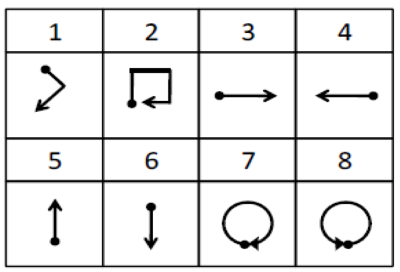
\includegraphics[scale = 0.9]{images/uWave_1.png} & 
            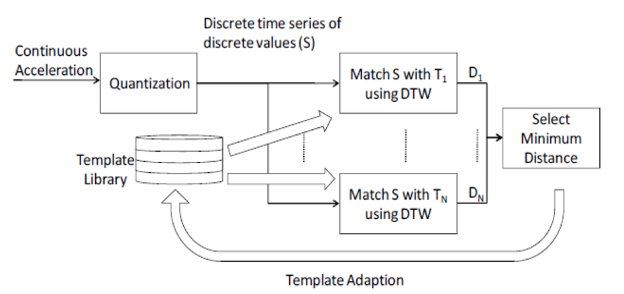
\includegraphics[scale = 0.9]{images/uWave_2.png} \\
        \end{tabular}
    \end{center}
\end{figure}

Теперь рассмотрим более детально данный алгоритм: \\
Его можно разбить на 3 части:
\begin{itemize}
    \item квантования данных, полученных с акселерометра.
    \item подбор соответствующего шаблона движения.
    \item адаптация шаблона (на рисунке ниже представлена более детальная схема работы).
\end{itemize}

Основной частью в алгоритме является другой алгоритм, называющийся «Динамической Трансформацией шкалы времени» («Dynamic Time Warping») -- он позволяет сравнить две последовательности (причем он может учитывать скорость изменения данных), например, данных алгоритм часто используют для распознавания речи. Если же более детально посмотреть на алгоритм «DTW», то он находит расстояние Левенштейна между последовательностью, записанной текущим жестом, и последовательностью эталонного жеста.

Последним шагом алгоритма является адаптация шаблона. Так как способ реализации жеста меняется от времени к времени, даже если этот жест будет исполнять один и тот же человек, следовательно нам нужно постоянно корректировать эталонный жест. Поэтому применяется незамысловатый алгоритм для поддержания актуальности жестов: для каждого эталона мы храним по две вариации его исполнения, и каждый новый способ, удачно распознанный, заменяет более старый из уже существующих двух.

Также стоит рассмотреть статические методы распознавнаия движений:
\begin{itemize}
    \item Например, Скрытие Марковские Цепи, который базируется на вероятностной интерпретации эталонов жестов для моделирования траектории жеста. При этом перед тем, как запустить алгоритм, следует провести предобработку входящих данных двумя фильтрами: первый -- отбрасывает вектора данных, которые не вносят значимый вклад в характеристику движения или жеста, второй – устраняет векторы данных, которые примерно похожи на предыдущий. Данный алгоритм неправильно классифицирует около $4-5 \%$ моделей, то есть в $95-96 \%$  случаев мы получим правильный результат, что весьма неплохо.
    \item Также имеем достаточно популярный метод: метод опорных векторов. Его основная идея перевод исходных векторов в пространство большей размерности и нахождение разделяющей гиперплоскости с максимальным зазором в этом пространстве. Соответственно две параллельные гиперплоскости будут находиться по обе стороны от разделяющей гиперплоскости. (Но суть работы с жестами заключается в том, чтобы строить множество разделяющих гиперплоскостей, чтобы была возможность поступающий жест определить к своему классу). При этом точность данного метода может достигать $98 \%$.
\end{itemize}

Подводя итог данному анализу, можно скзаать, что знание внутреннего устройства схожих алгоритмов, уже дало нам информацию о надобности фильтрации входных данных, а также помогло ускорить реализацию различных частей, так как мы могли ориентироваться на готовые решения.

\section{Теоретическая часть. Описание выбранных и разработанных методов, алгоритмов}
\subsection{Сбор данных (Савосин Артем, Гусев Владислав, Вишневский Глеб, Макаров Максим, Самарин Артем)}
Для работы по обучению модели, классифицирующей жесты, необходимо было собрать данные с этими жестами. Предположив, что жесты пользователей будут различаться в зависимости от их возраста, пола, физических особенностей, было принято решение собрать записи движений разных пользователей. Удалось записать движения 10 пользователей, 6 персон женского пола, 4 мужского, 5 пользователей старшей возрастной группы.

Также был учтен факт использования пользователями жестов с различными количествами тактов(разделение данных по разным группами в зависимостиот количества тактов).

Суммарно мы получили 600 различных движений.
Данные заранее были случайным образом разбиты на две группы - для тренировки модели и для проверки ее точности.

\begin{figure}[H]
    \center{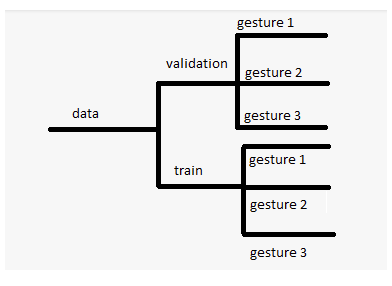
\includegraphics[scale = 1]{images_sav/data.png}}
\end{figure}


\subsection{Создание механизма 
сглаживания и фильтрации данных акселерометра и 
гироскопа (Агаев Фархат)}
Моей главной задачей являлось написть фильтр, 
который сможет сгладить данные и избавиться от шума.
Чтобы применить правильный фильтр нужно понять природу шума, 
почему датчик акселерометра искажает данные.
\subsubsection{Природа шума}
Для начала нарисуем график по трем осям (начнем с акселерометра), 
когда телефон лежит на столе. Посмотрим есть какие-либо перепады

\begin{figure}[H]
    \begin{center}
        \begin{tabular}{cc}
            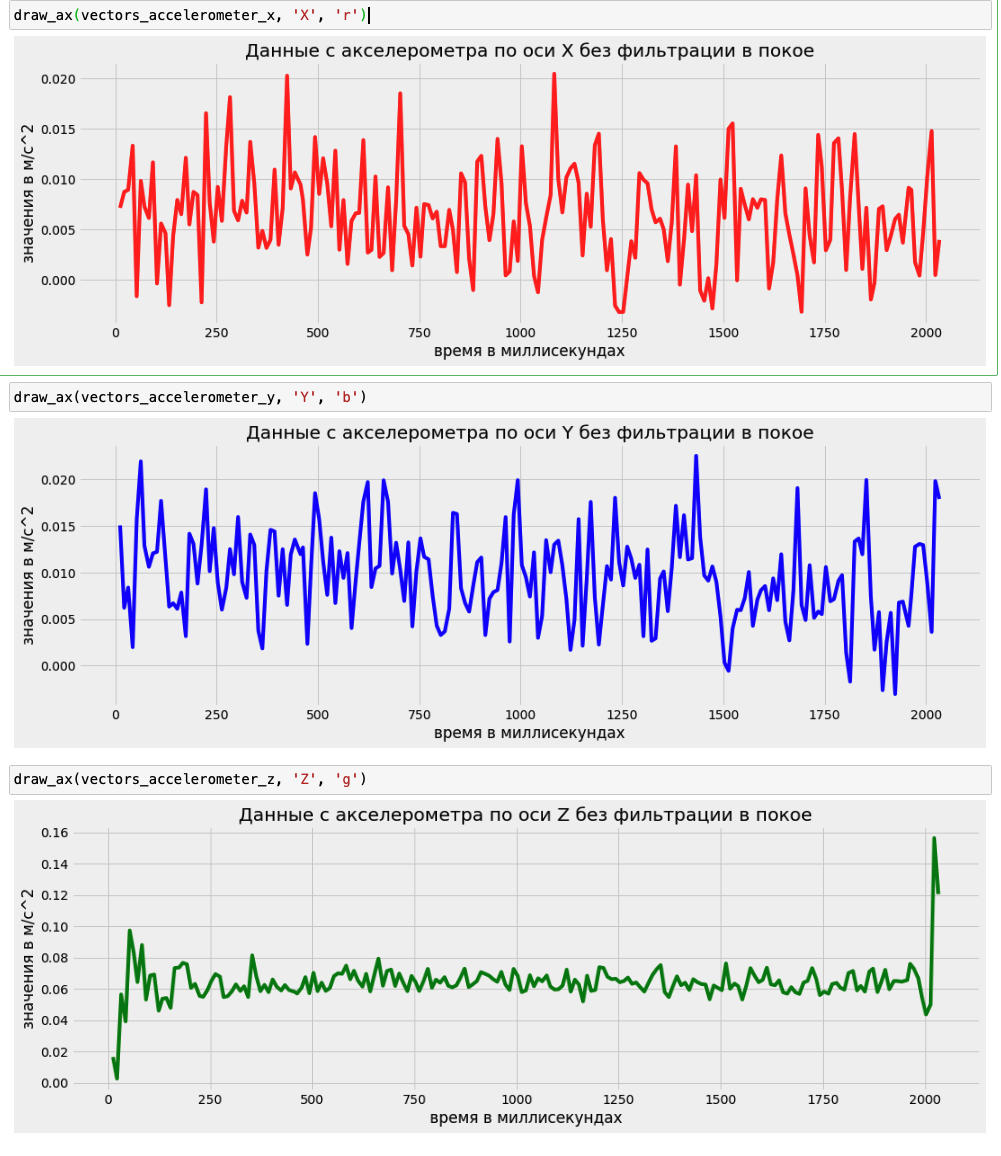
\includegraphics[width=0.75\textwidth]{farim/shakeee} & 
        \end{tabular}
    \end{center}
\end{figure}

На графике хорошо видно, что есть высокочастотные сигналы, 
когда телефон просто лежит на столе от -0.025  до 0.025 $\text{м}/\text{с}^2$. То есть
погрешность уже состовляет более двух процентов. 

\begin{figure}[H]
    \begin{center}
        \begin{tabular}{cc}
            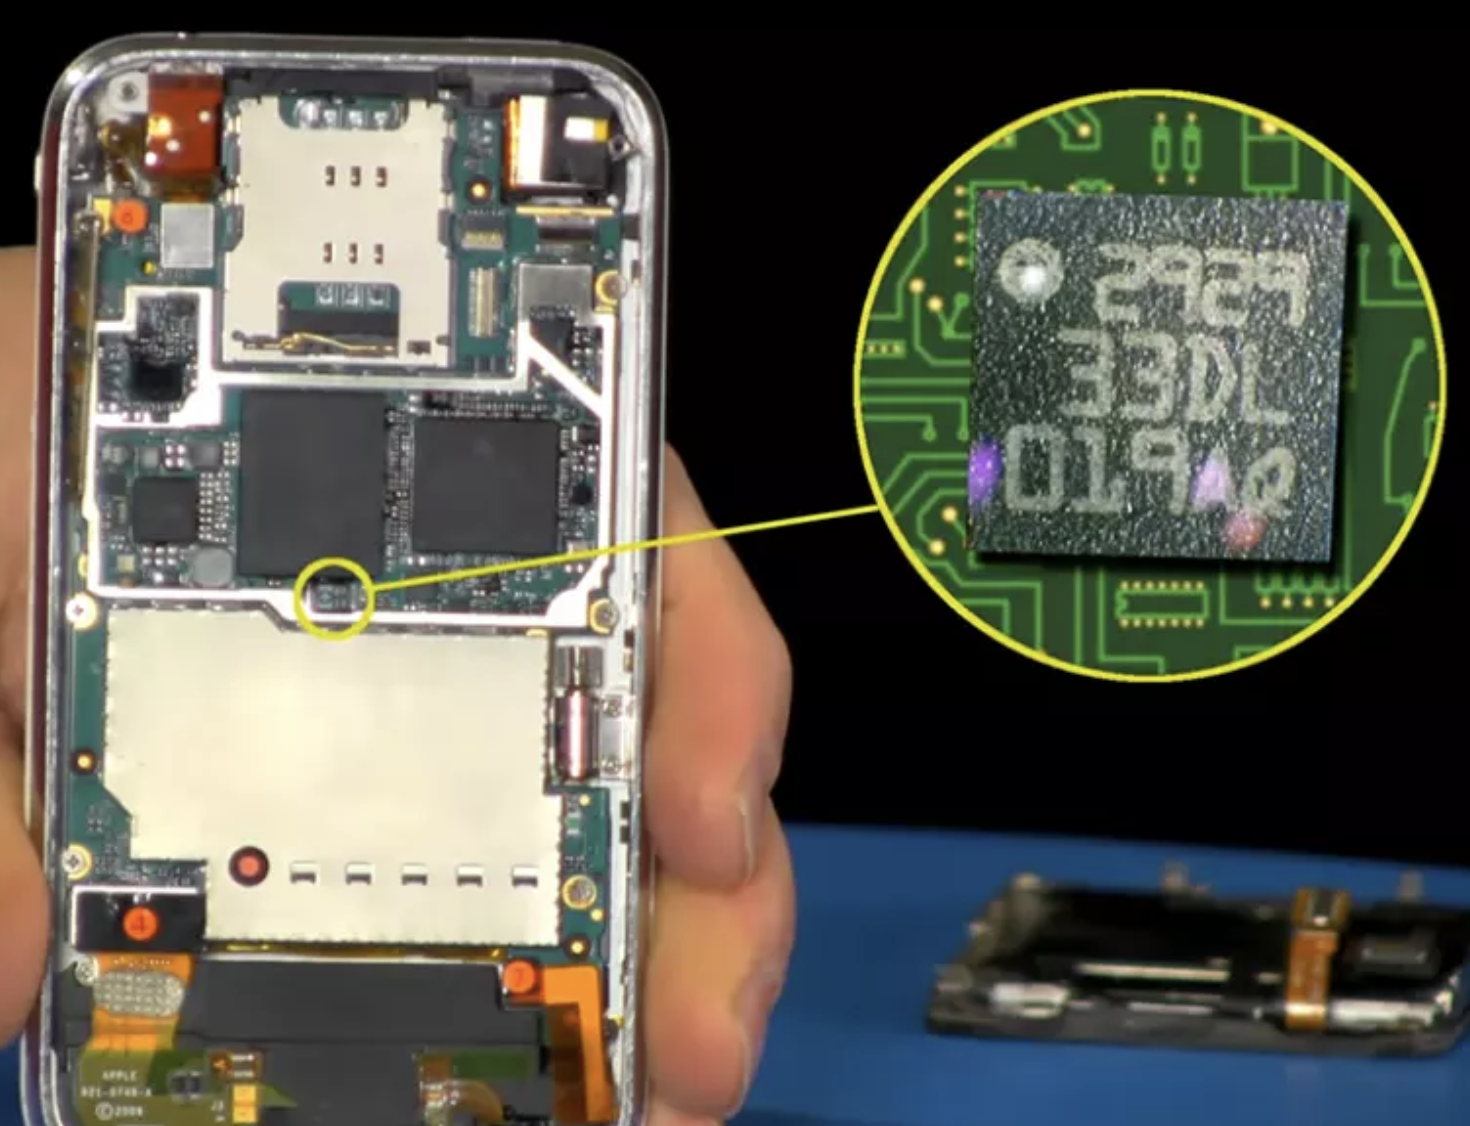
\includegraphics[width=0.5\textwidth]{farim/im2} & 
            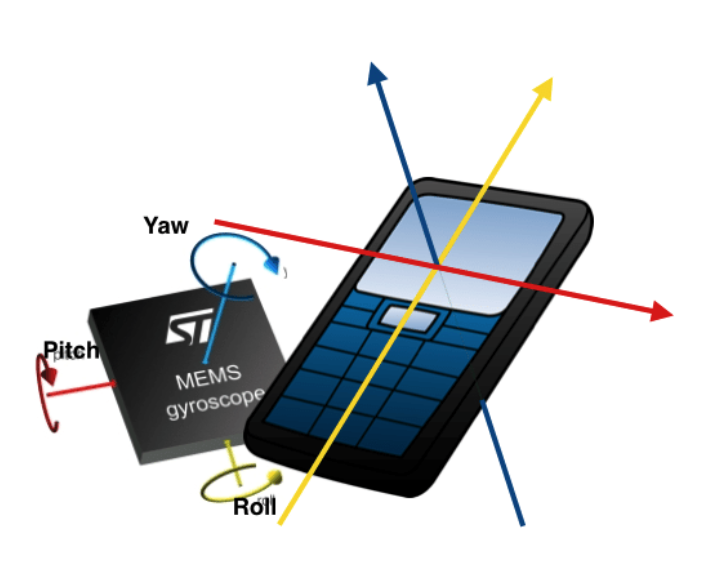
\includegraphics[width=0.5\textwidth]{farim/im3}
        \end{tabular}
    \end{center}
    \caption{изображение датчика акселерометра и гироскопа.}
\end{figure}
Также на величину выходного сигнала акселерометра в основном влияют:
\begin{enumerate}
    \item температура окружающей среды и места крепления акселерометра (температурные погрешности);
    \item внешние электро-магнитные поля (погрешности от магнитного поля);
    \item вибрация и угловые колебания основания (вибрационные погрешности);
    \item частотные характеристики акселерометра (частотные погрешности);
    \item гистерезис показаний (одна из составляющих нелинейности).
\end{enumerate}



\newpage
Теперь взглянум на график разных жестов 
\begin{figure}[H]
    \begin{center}
        \begin{tabular}{cc}
            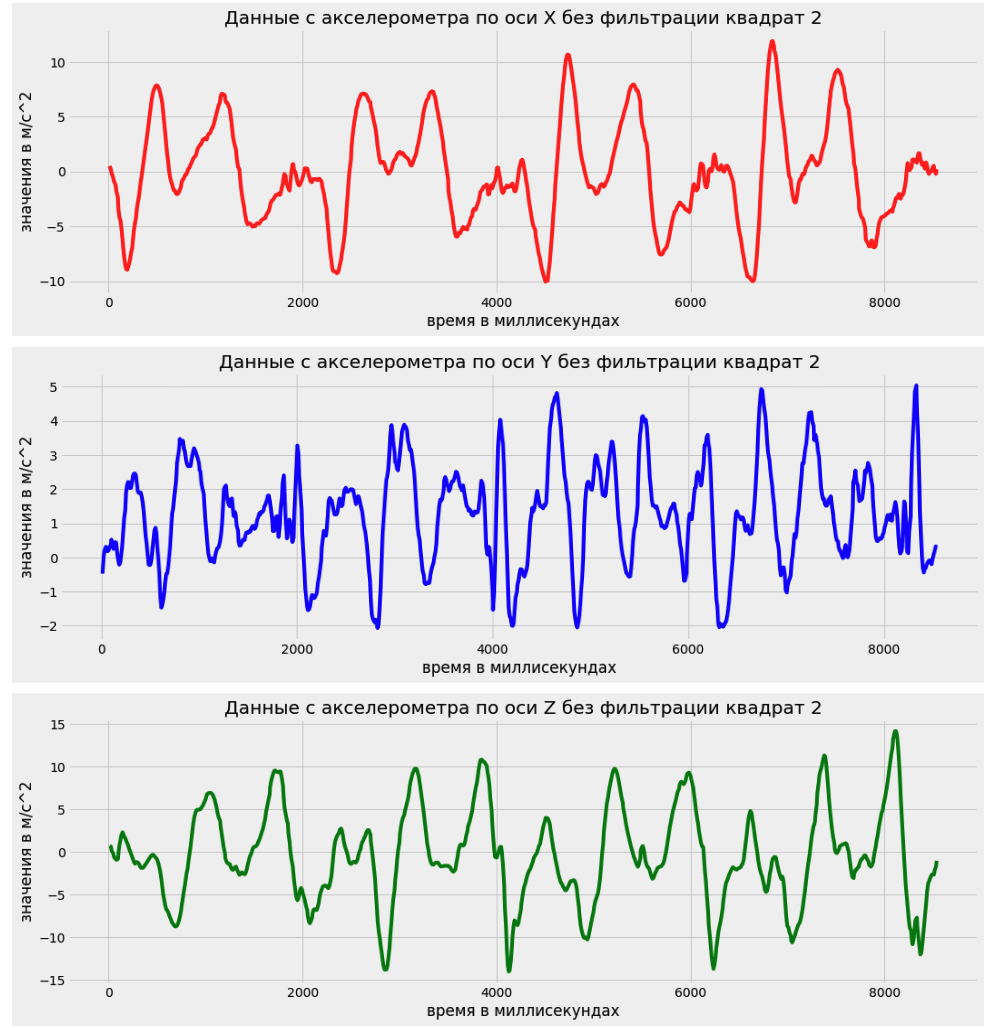
\includegraphics[width=1\textwidth]{farim/sq} & 
        \end{tabular}
    \end{center}
\end{figure}

Хорошо видны всплески и  резкие искажения, их нужно будет сгладить

\begin{figure}[H]
    \begin{center}
        \begin{tabular}{cc}
            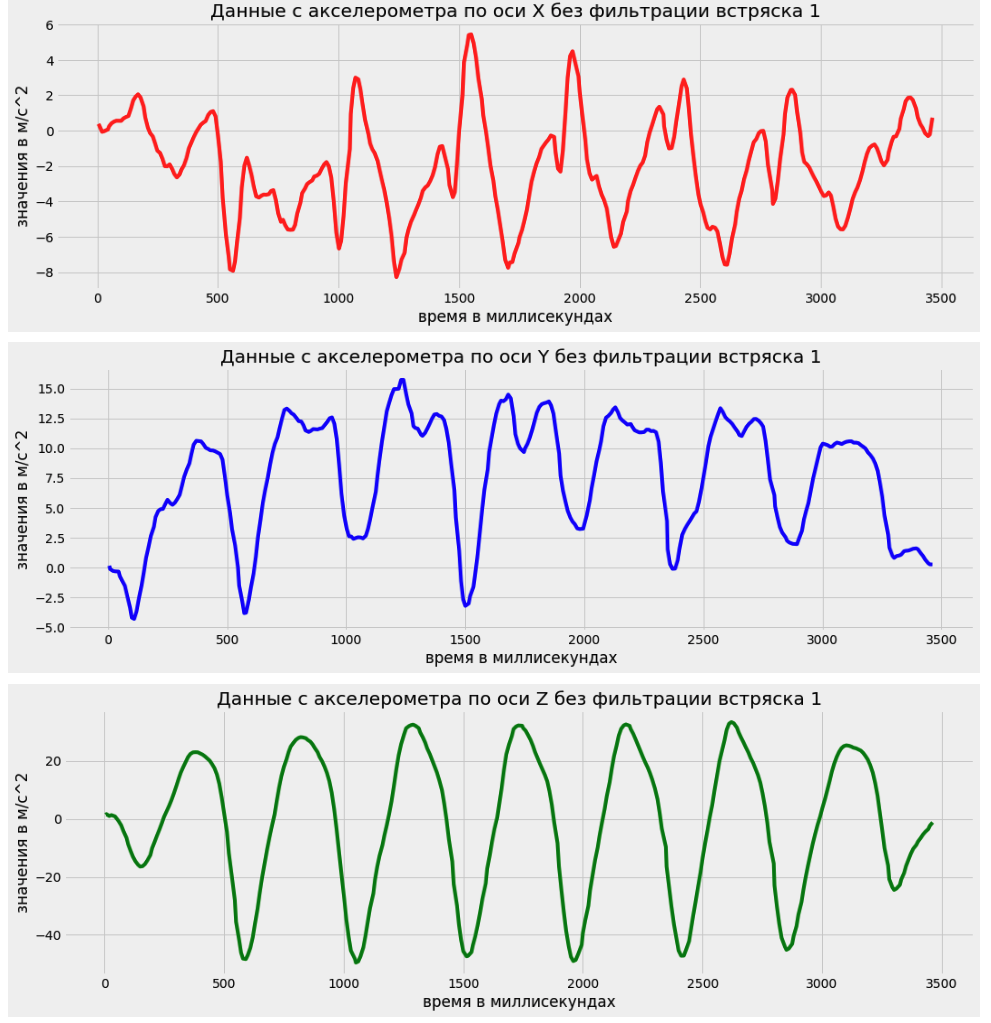
\includegraphics[width=1\textwidth]{farim/shakeeee.png} & 
        \end{tabular}
    \end{center}
\end{figure}

Когда происходит встряска график получается более гладкий особенно по оси Z.
Теперь рассмотрим жест круг, для больше точности и понимания
Посмотрим графики несколько кругов, полученных при разной скорости их реализации.
Круги будут идти с возрастающей скоростью.
Также рассмотрим круги с разными радиусами, попробуем понять, насколько сильно будут портиться данные.

\begin{figure}[H]
    \begin{center}
        \begin{tabular}{cc}
            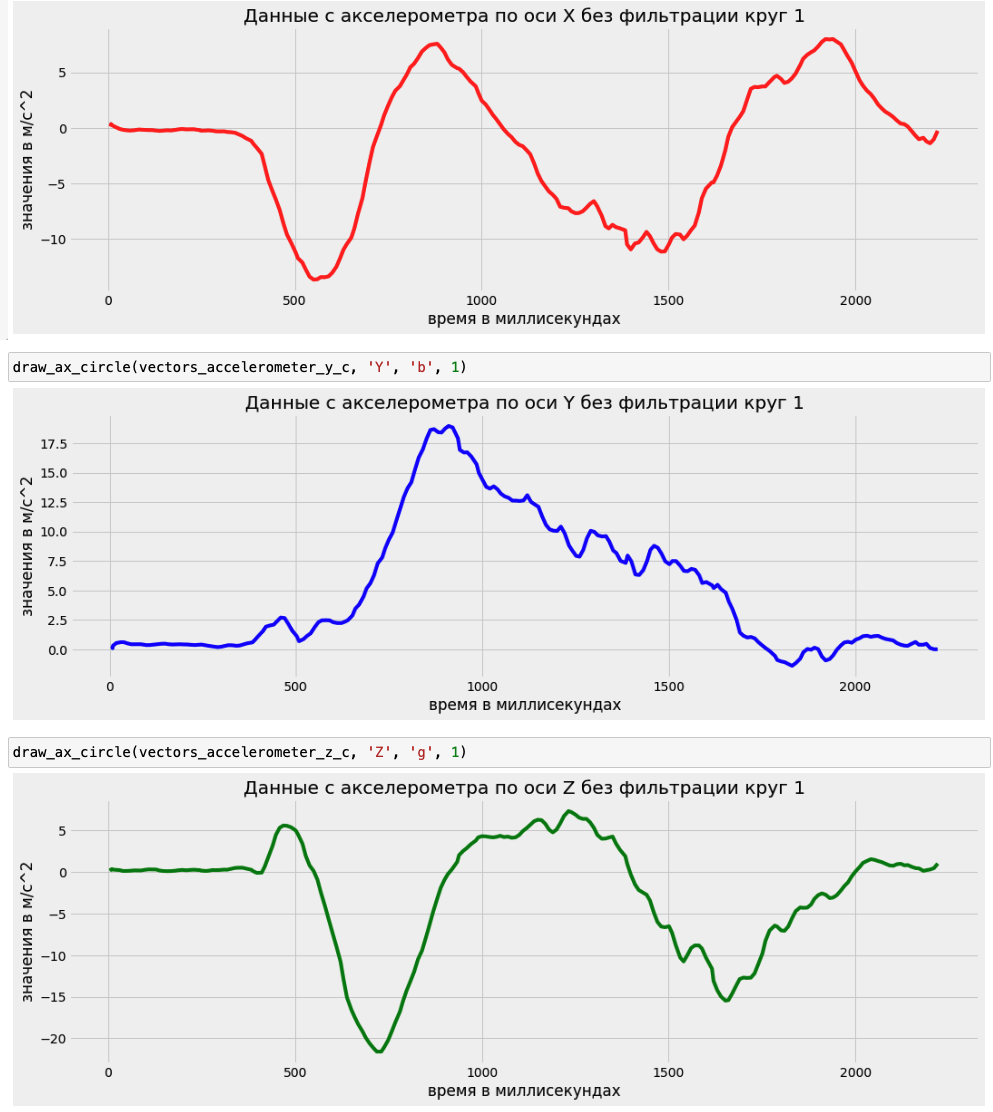
\includegraphics[width=1\textwidth]{farim/cirx} & 
        \end{tabular}
    \end{center}
\end{figure}


\begin{figure}[H]
    \begin{center}
        \begin{tabular}{cc}
            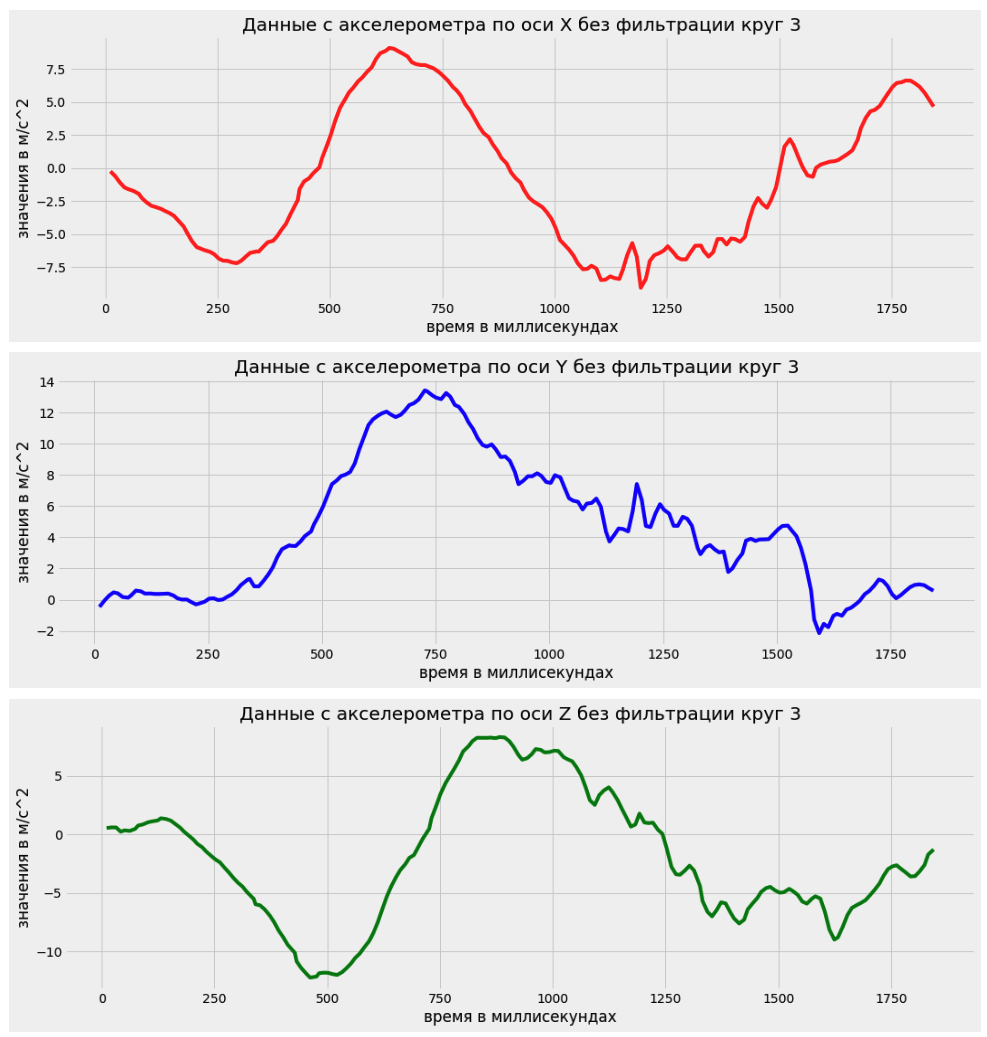
\includegraphics[width=1\textwidth]{farim/im4.png} & 
        \end{tabular}
    \end{center}
\end{figure}


\newpage
\begin{figure}[H]
    \begin{center}
        \begin{tabular}{cc}
            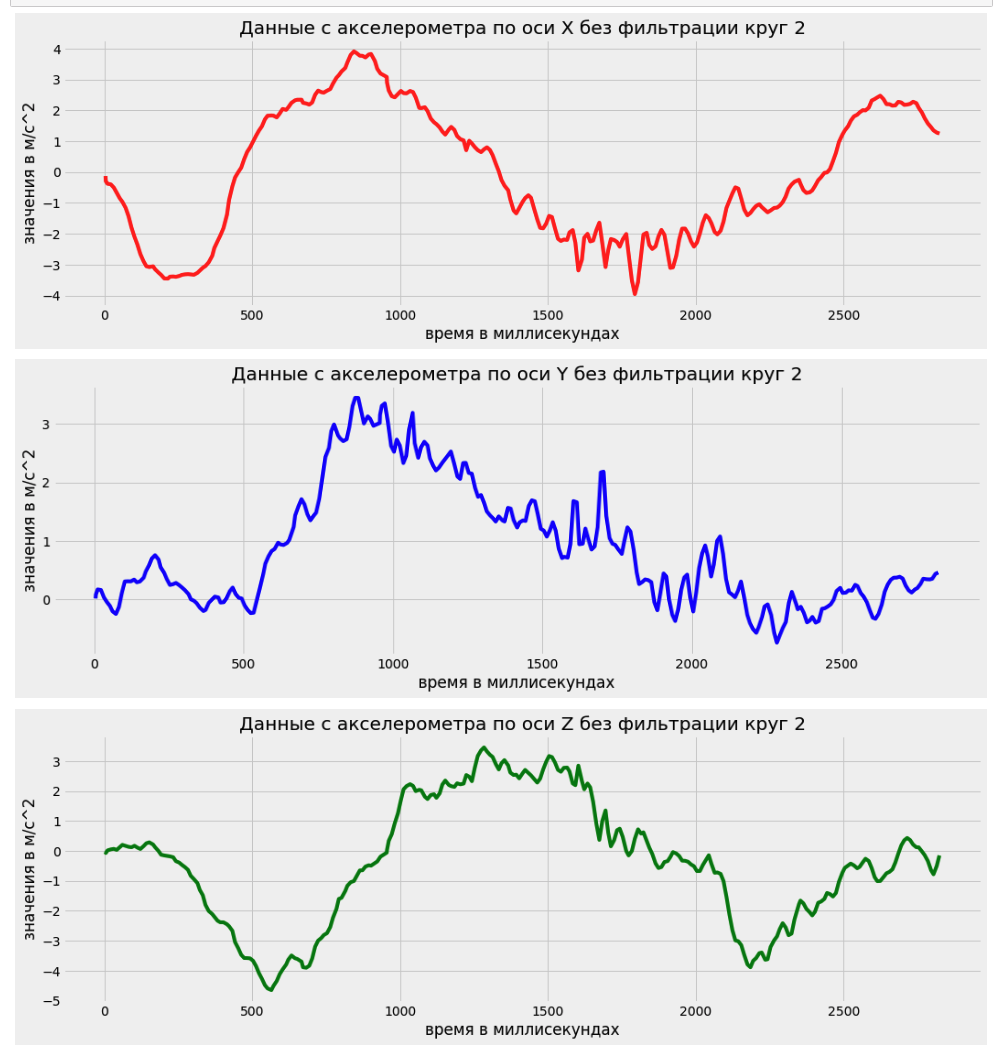
\includegraphics[width=1\textwidth]{farim/im5.png} & 
        \end{tabular}
    \end{center}
\end{figure}


\begin{figure}[H]
    \begin{center}
        \begin{tabular}{cc}
            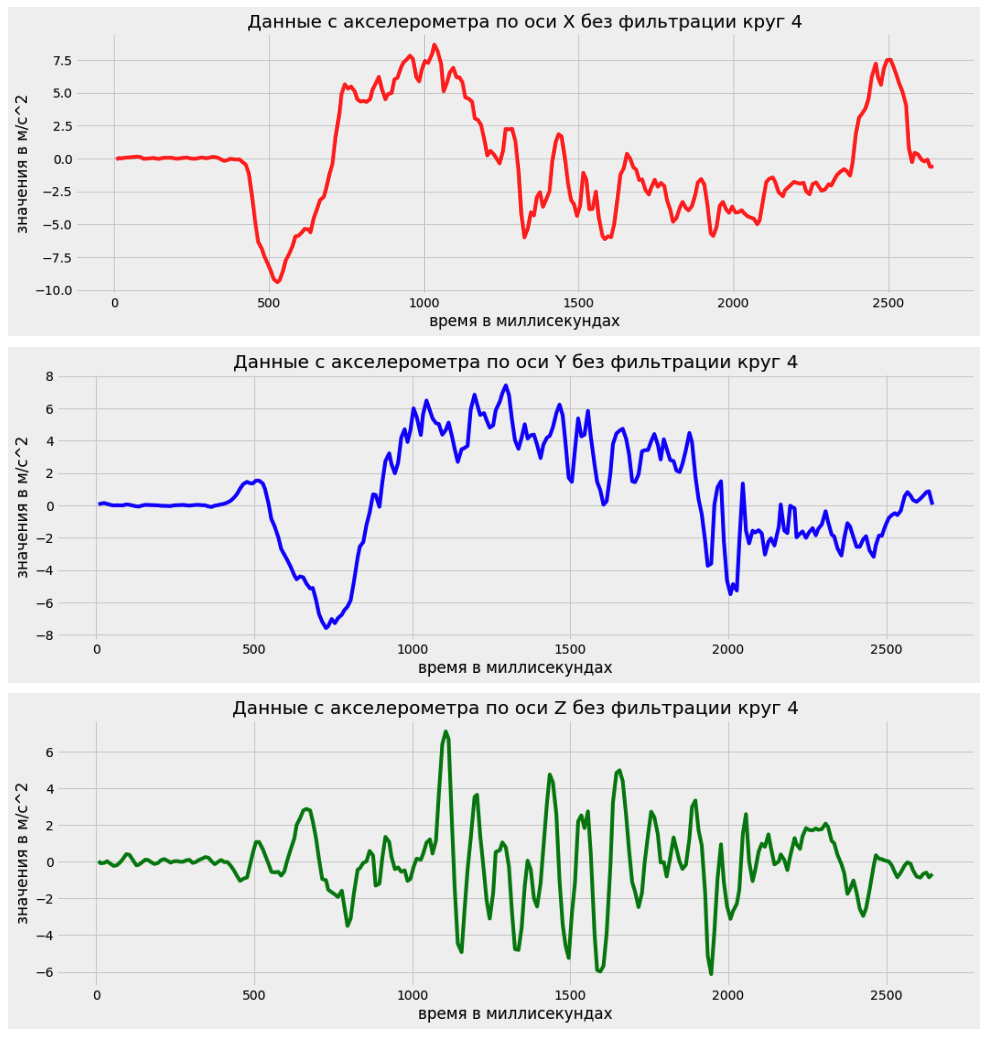
\includegraphics[width=1\textwidth]{farim/im6.png} & 
        \end{tabular}
    \end{center}
\end{figure}


\begin{figure}[H]
    \begin{center}
        \begin{tabular}{cc}
            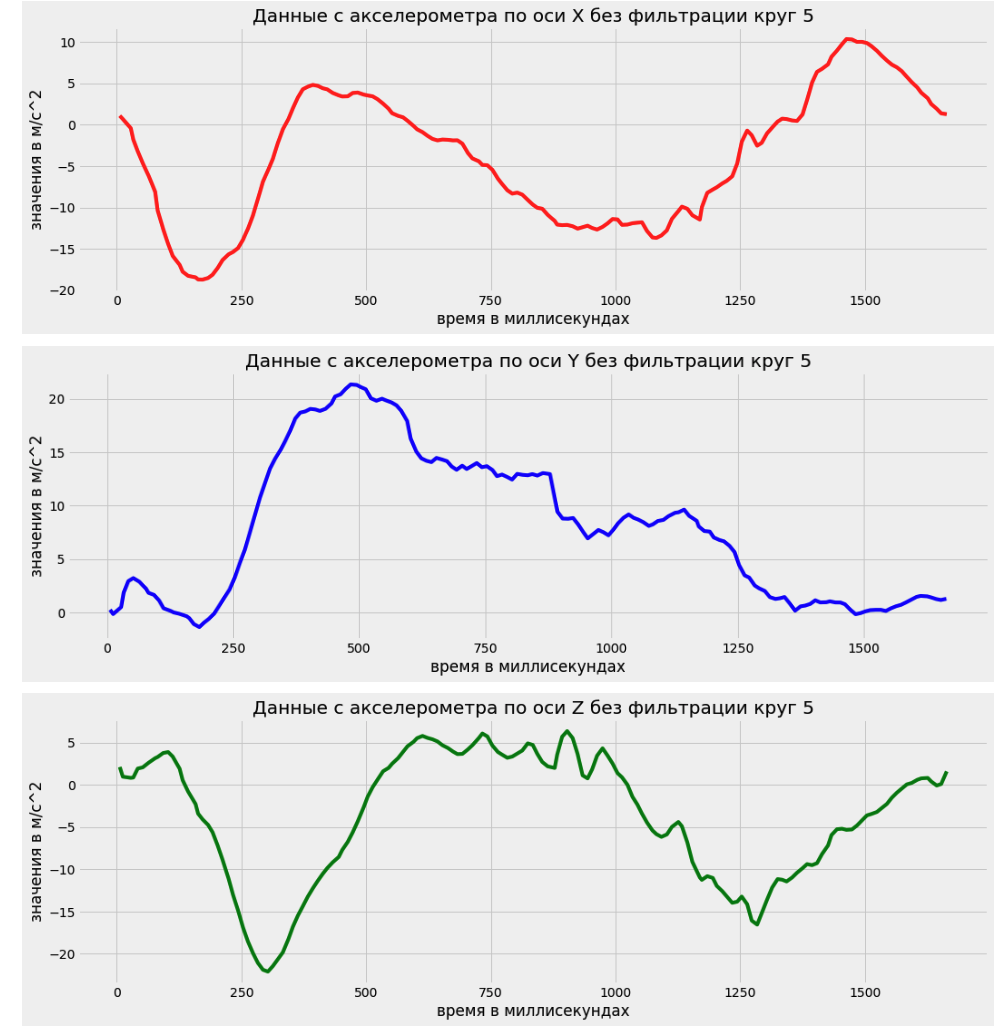
\includegraphics[width=1\textwidth]{farim/im7.png} & 
        \end{tabular}
    \end{center}
\end{figure}
Как мы можем заметить главная проблема - высокие частоты и очень резкие переходы в этом случае.
для нас идеально подойдет фильтр нижних частот.






\newpage
\subsubsection{Принцип работы}

Это фильтр, который пропускает сигналы с 
частотой ниже выбранной частоты среза и 
ослабляет сигналы с частотами выше, чем частота
среза.
В нашем случае я подобрал частоту среза равную  0.6 Гц (Опытным путем построения графиков так, чтобы 
не сильно уходить от данных полученных непосредственно от датчика и максимально хорошо сгладить данные)
Фильтр реализован с помошью питоновских библиотек scipy, numpy (код есть на гитхабе) 
Воспользуемся фильтром и посмотрим результат работы
\begin{figure}[H]
    \begin{center}
        \begin{tabular}{cc}
            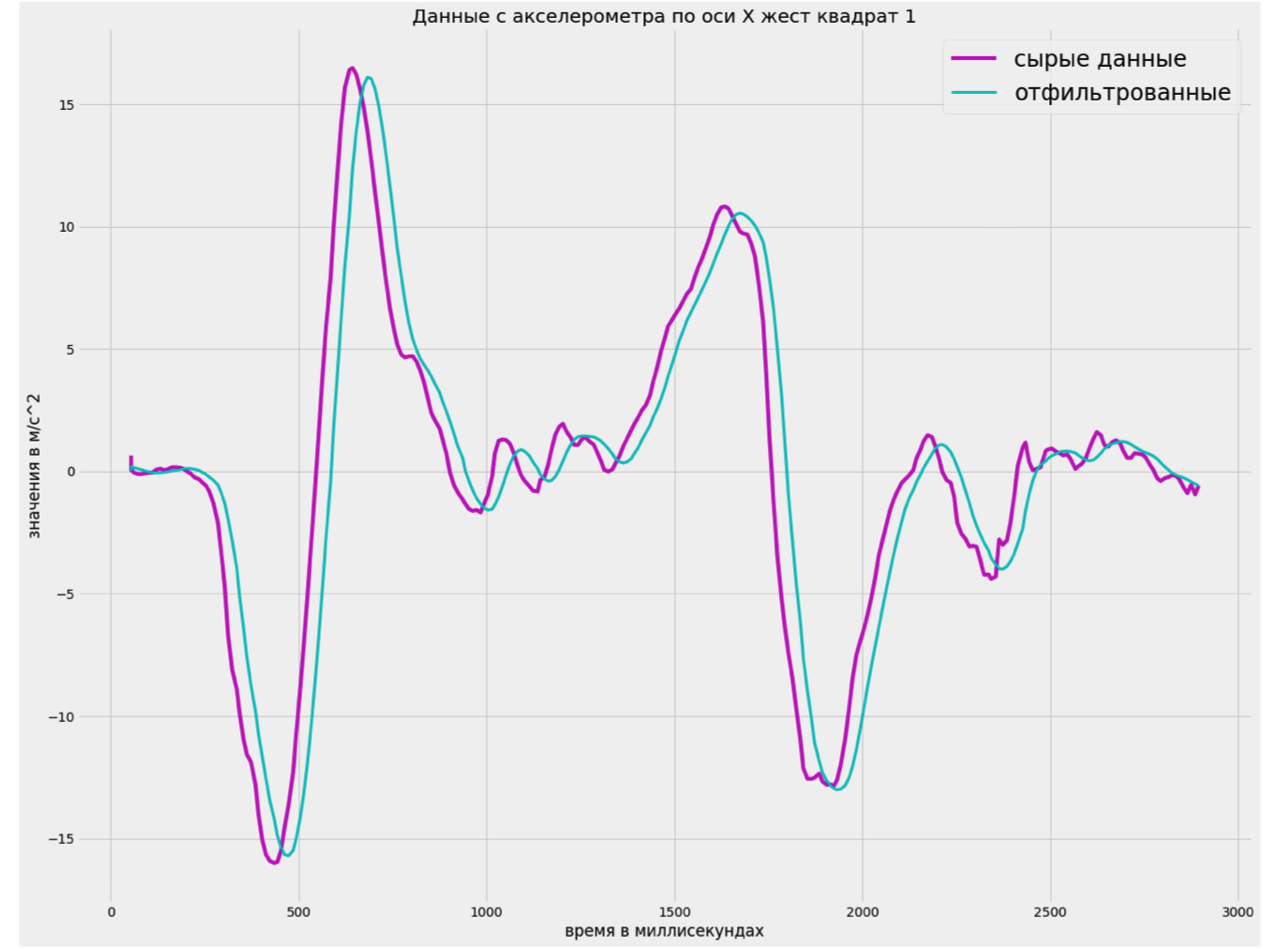
\includegraphics[width=0.75\textwidth]{farim/squares} & 
        \end{tabular}
    \end{center}
\end{figure}
\begin{figure}[H]
    \begin{center}
        \begin{tabular}{cc}
            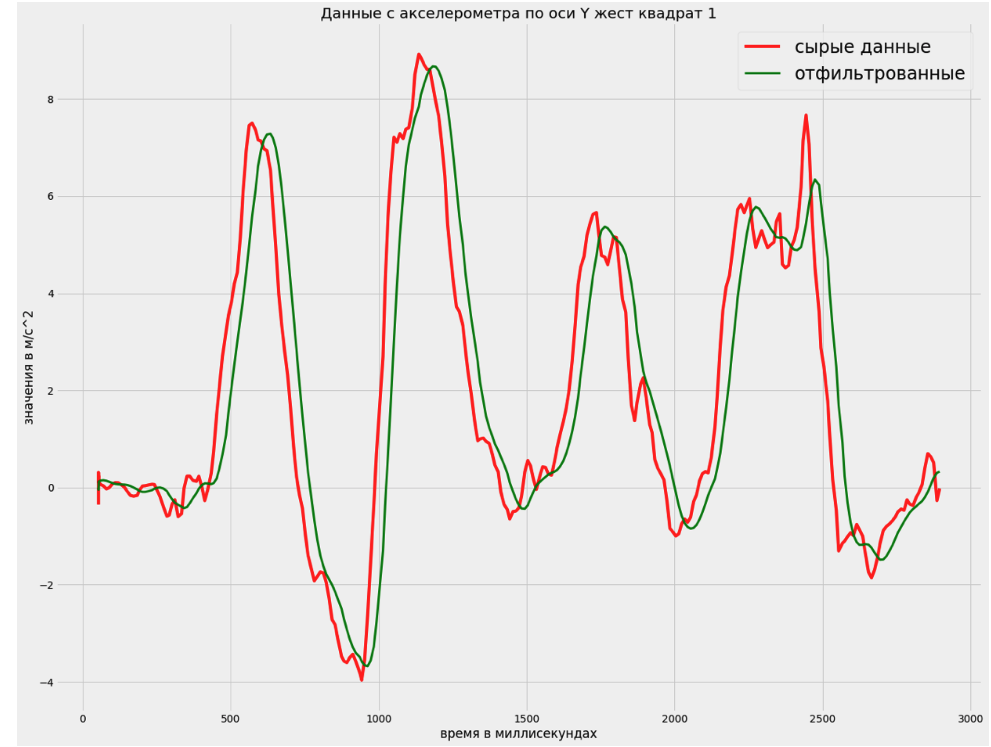
\includegraphics[width=0.75\textwidth]{farim/sqxres} & 
        \end{tabular}
    \end{center}
\end{figure}

\begin{figure}[H]
    \begin{center}
        \begin{tabular}{cc}
            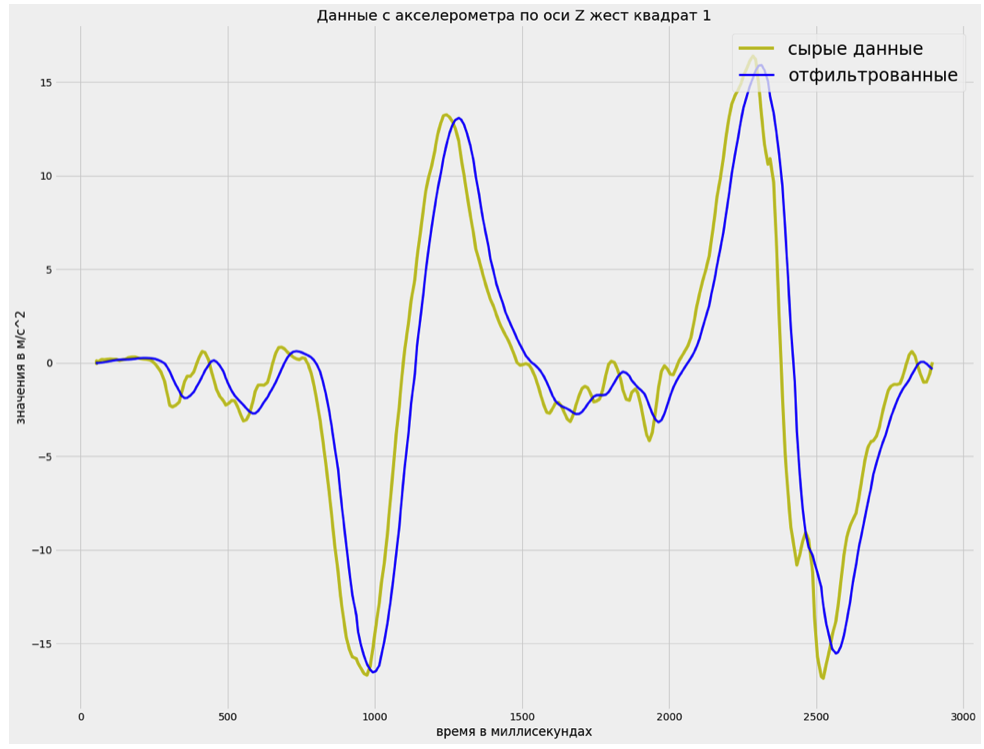
\includegraphics[width=0.75\textwidth]{farim/sqzres} & 
        \end{tabular}
    \end{center}
\end{figure}

\begin{figure}[H]
    \begin{center}
        \begin{tabular}{cc}
            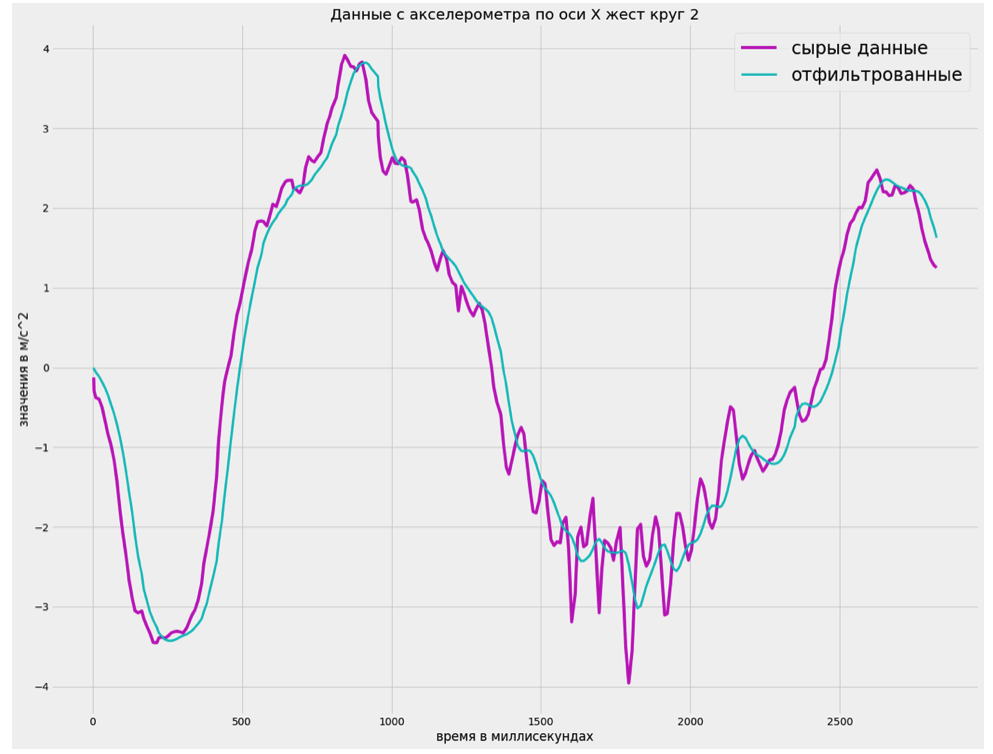
\includegraphics[width=0.75\textwidth]{farim/cirxres.png} & 
        \end{tabular}
    \end{center}
\end{figure}

\begin{figure}[H]
    \begin{center}
        \begin{tabular}{cc}
            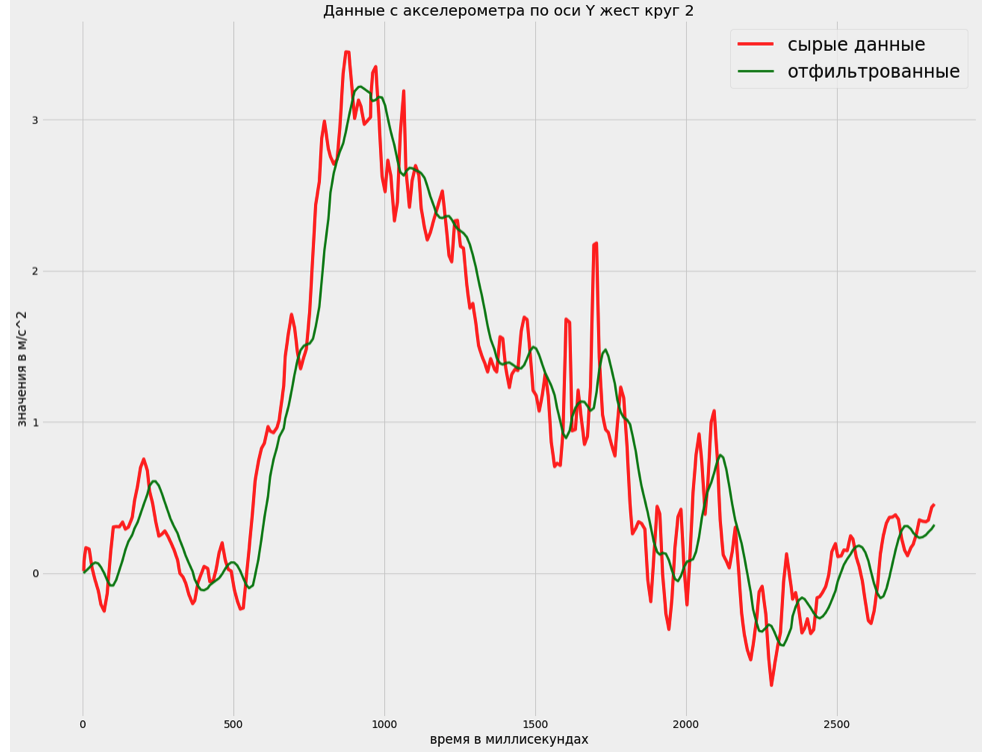
\includegraphics[width=0.75\textwidth]{farim/ciryres.png} & 
        \end{tabular}
    \end{center}
\end{figure}


\begin{figure}[H]
    \begin{center}
        \begin{tabular}{cc}
            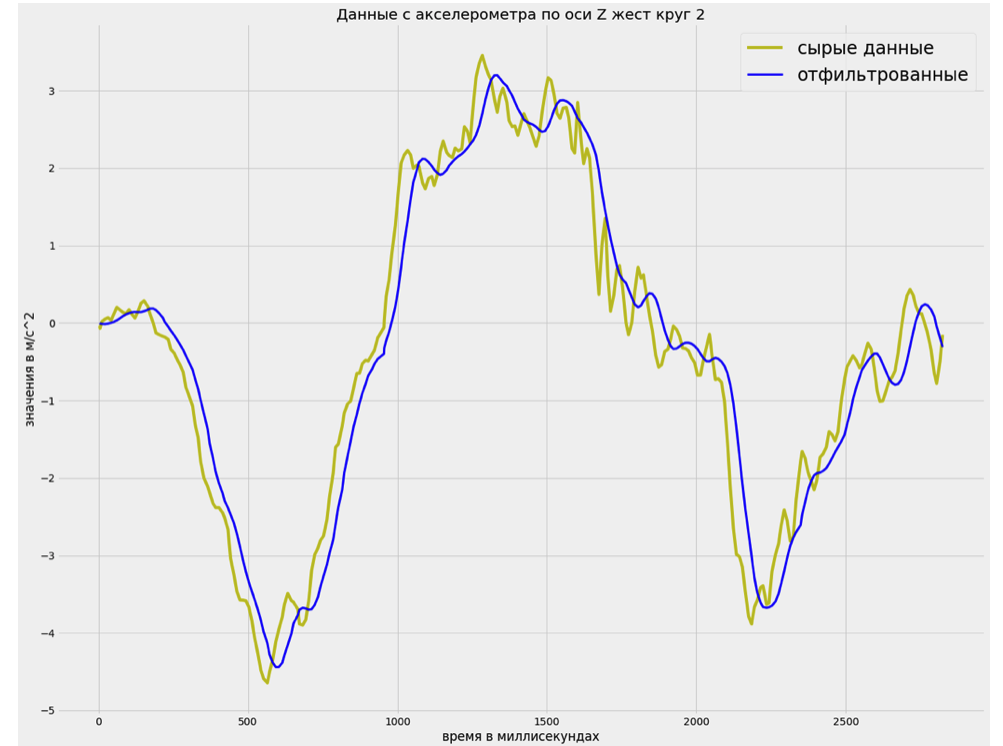
\includegraphics[width=0.75\textwidth]{farim/cirzres.png} & 
        \end{tabular}
    \end{center}
\end{figure}

\begin{figure}[H]
    \begin{center}
        \begin{tabular}{cc}
            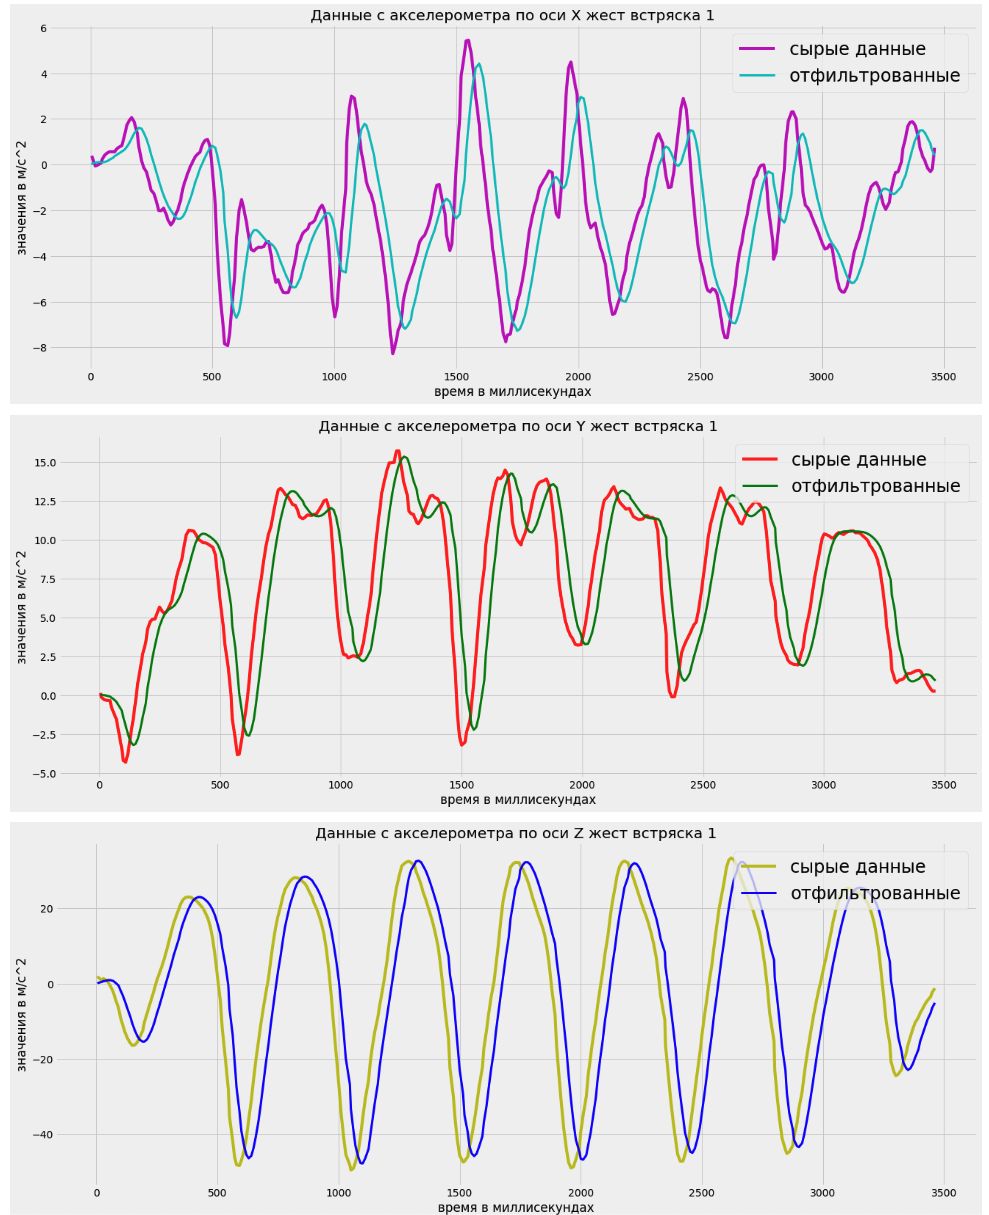
\includegraphics[width=1\textwidth]{farim/shak.png} & 
        \end{tabular}
    \end{center}
\end{figure}


\textbf{Итоги работы:} На графика хорошо видно, 
что фильтр справился со своей задачей. Мы получили более гладкий сигнал,

\section{Часть Гусева Владислава Сергеевича}

\subsection{Теоретическая часть. Описание выбранных и/или разработанных методов, алгоритмов, моделей данных, методик и т.п.}
Изначально передо мной стояла задача исследования уже готовых решений, доступных в открытых источниках и выделить общую структуру, по которой они работают.

Считаю нужным отметить, что нас устраивают алгоритмы, которые работают только с аппаратными составляющими – акселерометром и гироскопом.

Сразу можно разделить алгоритмы по распознаванию жестов на 2 категории: классификация по 3D графику или 3D фигуре, классификация по некому внешнему подобию 3D фигуры (в нашем случае 2D проекции 3D фигуры).

Но методы, использующие 3D модель для идентификации жестов, обрабатывают сложные трехмерные поверхности и классифицируют жесты с помощью нейронных сетей. Следовательно, недостатком такого метода является большая ресурсоемкость, так как построение самой модели, обучение нейронной сети и ее использование могут потребовать значительных ресурсов, что недопустимо при разработке технологии для мобильных устройств. Поэтому было принято решение оставить классификацию движений по 2D проекции.

Далее была выявлена общая концепция схожих алгоритмов:
\begin{enumerate}
    \item{Сбор информациии}
    \item {Фильтрация собранных данных}
    \item {Различная обработка собранных данных}
\end{enumerate}

Далее я выяснил, что все алгоритмы по распознаванию 2D жестов или движений можно разделить на два класса:
\begin{enumerate}
    \item основывающиеся на шаблонах – их суть в том, что они хранят эталонные движения или жесты, а далее производится их сравнение с произведенным движением при помощи различных метрик и второй: основывающиеся на моделях.
    \item Нахождение и выделение основных характеристик в поступающих данных и классификация этих характеристик.
\end{enumerate}

Далее вся разработка алгоритмов было произведена на Python, а именно в Jupyter Notebook, которая по итогу была перенесена на чистый Python.
Передо мной стояла главная задача -- выделить такты из общего движения телефоном, после чего усреднить все такты движений в единый жест, который уже смогли бы обработать мои члены команды.

для начала следовало проверить каждую ось на наличие цикличности, поэтому данные по каждой оси были изображены на плоскости (для проверки использовались все жесты с несколькими тактами):
\begin{figure}[H]
    \center{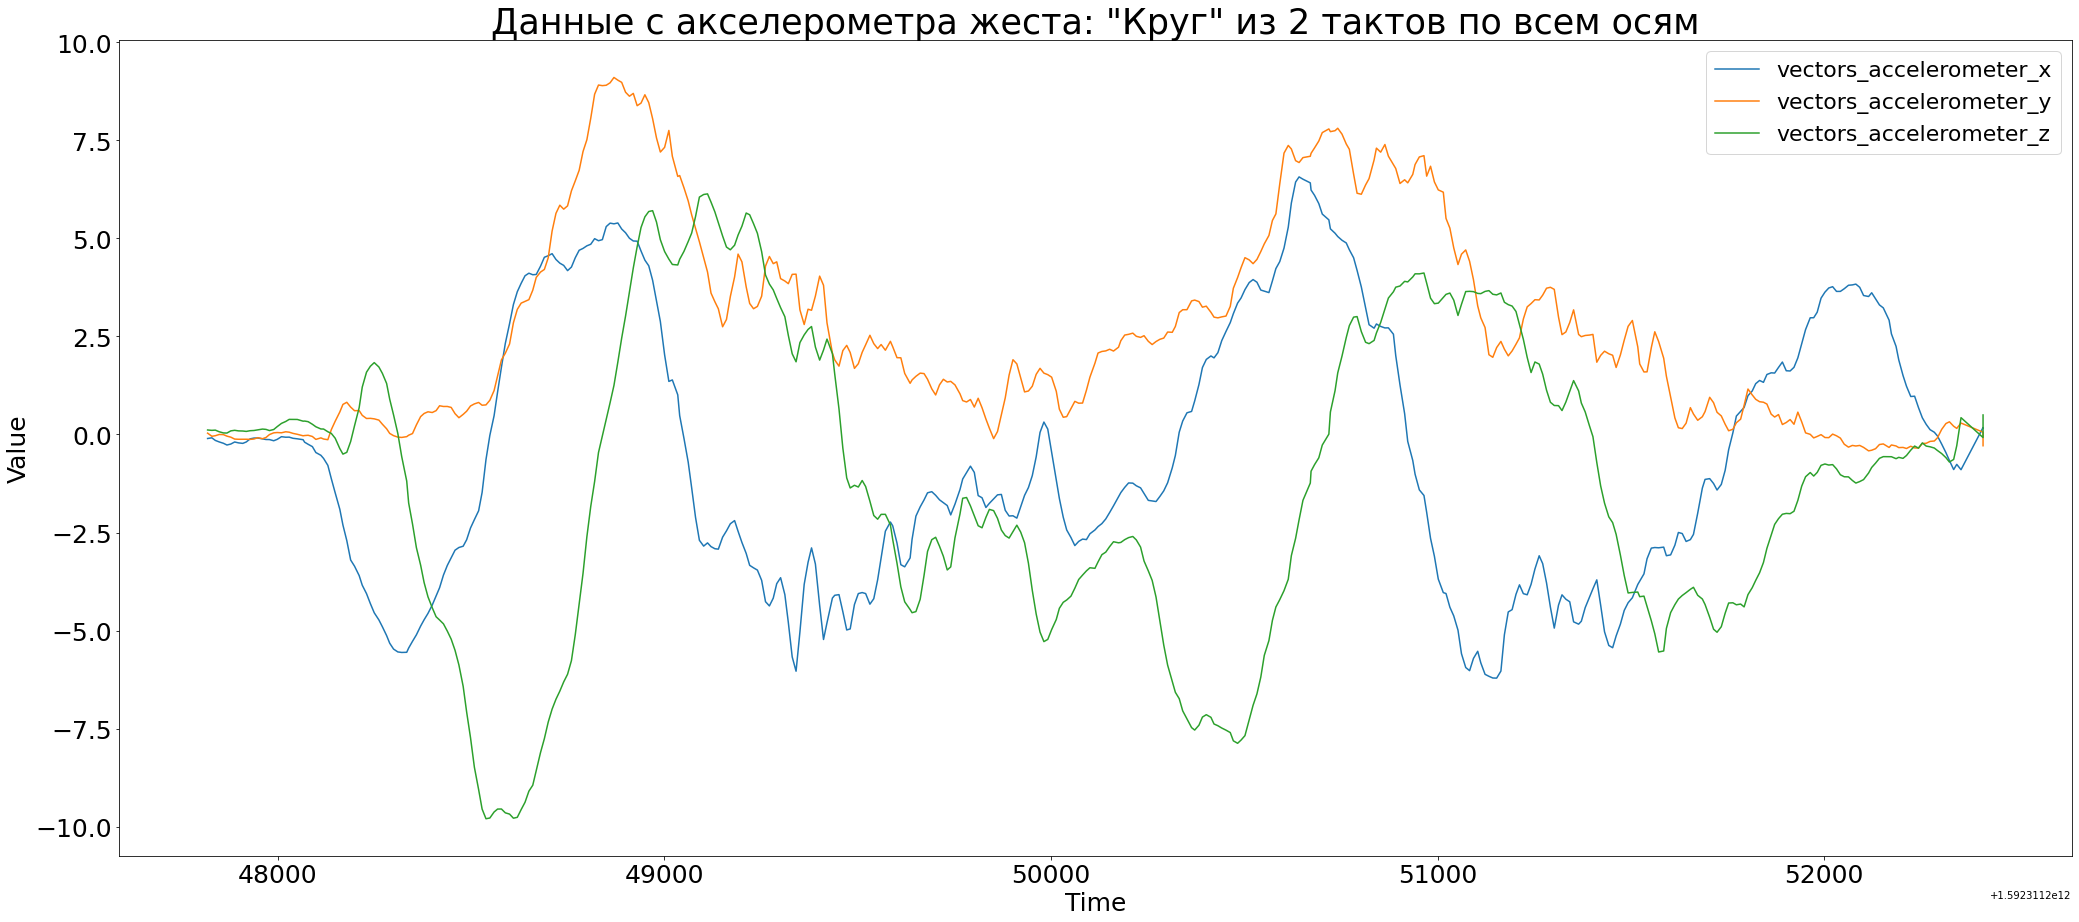
\includegraphics[width=15cm, height=8cm]{accelerometer_data_2_circle_xyz.png}}
    \center{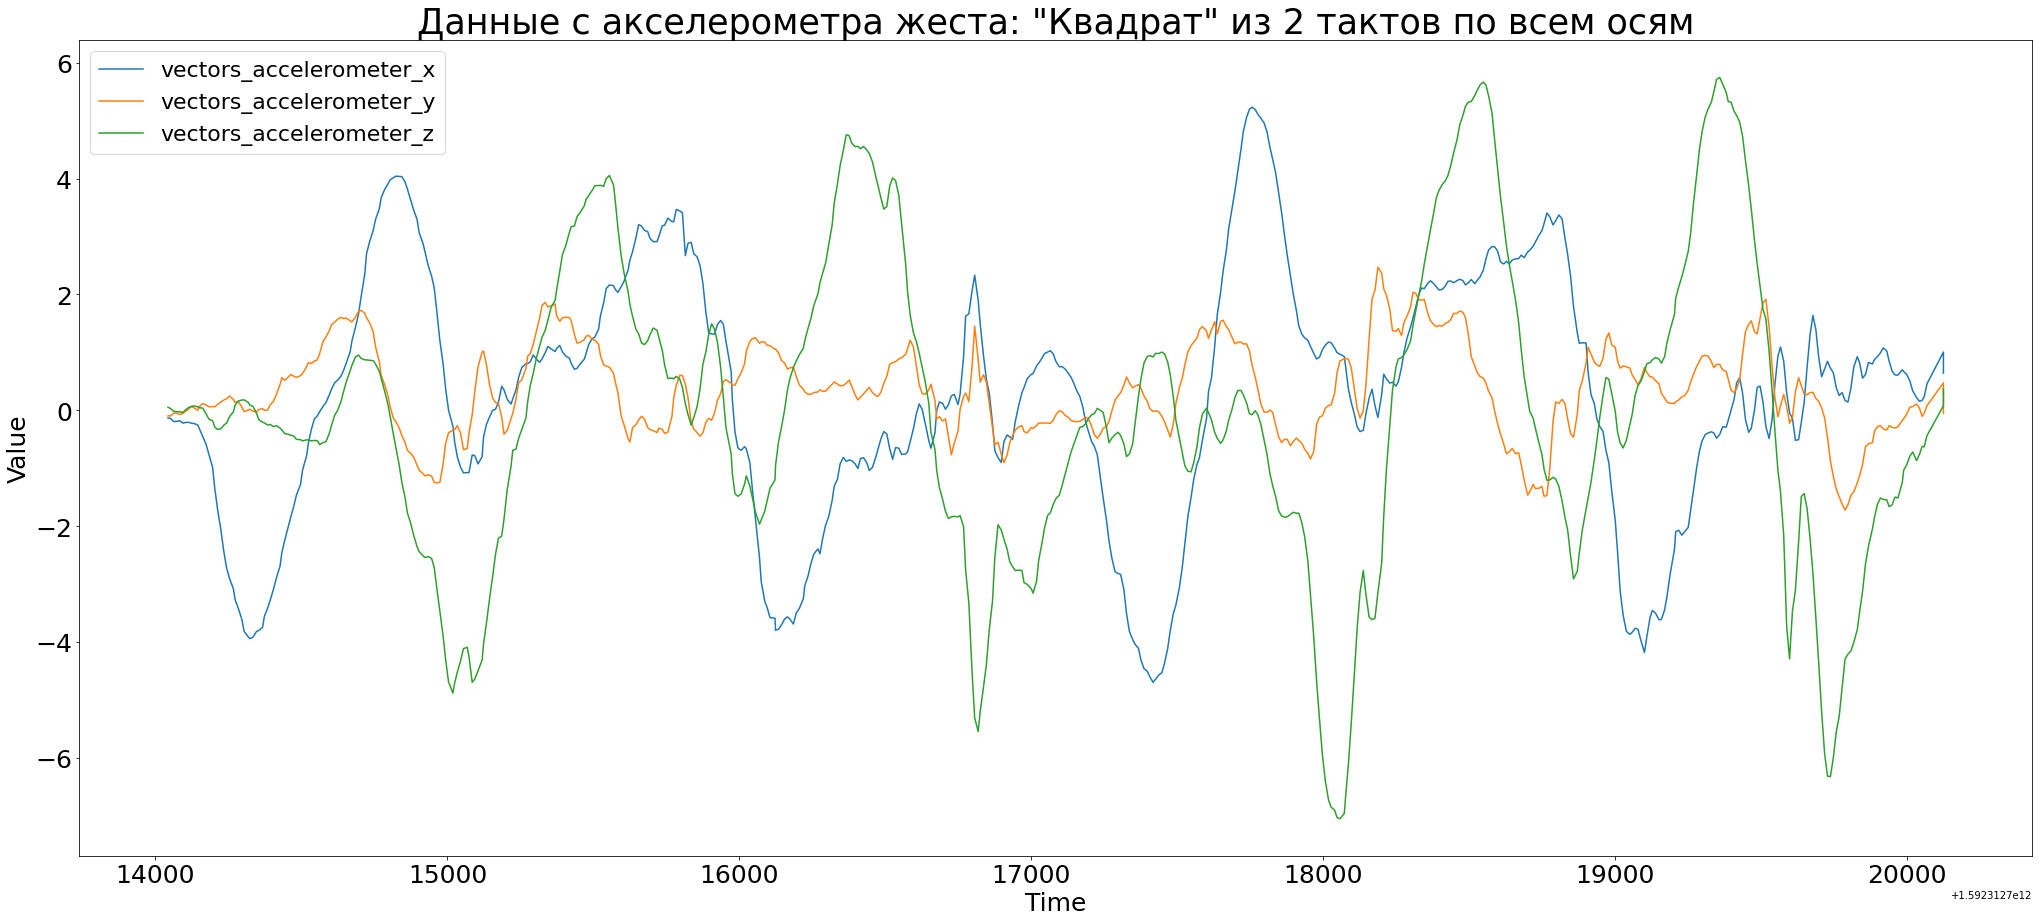
\includegraphics[width=15cm, height=8cm]{accelerometer_data_2_square_xyz.png}}
\end{figure}

После зрительного анализа легко заметить схожесть некоторых частей графиков, что дало положительный ответ на предположение о существовании схожих фрагментов по каждой из осей движения. Следовательно, я мог продолжить изучение выделения периодов временных рядов, но на этот раз уже одномерных.

\subsubsection*{Неудачные попытки}

Так как я получаю на вход трехмерный массив, то есть трехмерный временной ряд, то задча поиска цикличности в таком ряду сильно усложняется, поэтому мной было принято решение для начала выделить такты по каждой из осей.

Так как мы знаем, что в нашем ряде присутствует периоды (при этом они все полные – то есть очередной цикл не обрывается на каком-то месте, а выполняется до конца), а наши данные являются некоторой функцией $f(x)$, заданной на определенном отрезке, такую функцию можно представить в виде суммы гармонических функций, поэтому для их нахождения можно использовать преобразование Фурье (а именно, дискретное преобразование Фурье, так как наши данные не непрерывные). Преобразование Фурье
дает возможность представить непрерывную функцию $f(x)$ (в нашем случае показатели с датчиков), определенную на некотором отрезке в виде суммы бесконечного ряда тригонометрических функций (с разными амплитудами и фазами), что позволяет выявить периодические компоненты в данных (как раз то, что нам нужно).

По итогу мы бы получили спектр входных данных, а он может быть представлен суммой конечного числа гармонических составляющих. Но так было только теоретичеси, проверка данного алгоритма показала не совсем нужные результаты (схожих гармоник оказалось сликшом много), что не позволило корректно определять такты входных жестов.

\subsubsection*{Новый способ}
Был найден новый способ выделения тактов в жесте, по-прежнему задача стоит в выделение цикла в каждой из осей:
\subsubsection*{Устранение лишних шумов:}
Так как наше приложение записывает данные только по нажитю <<кнопки>>, то стоит учитывать тот факт, что сам жест будет начинаться не с начала записи данных, а с некоторого шума(то есть датчики будут находится в покое). Для удаление данного эффекта, который мог бы отразиться негативно на выделении тактов, уберем из общего массива данных по некоторому количеству элементов с начала и конца. То есть нам нужно идти с начала и с конца массива данных и убирать эелементы, пока они меньше $\alpha$. Для определения значения для $\alpha$ было проведено два эксперимента:

\begin{figure}[H]
    \center{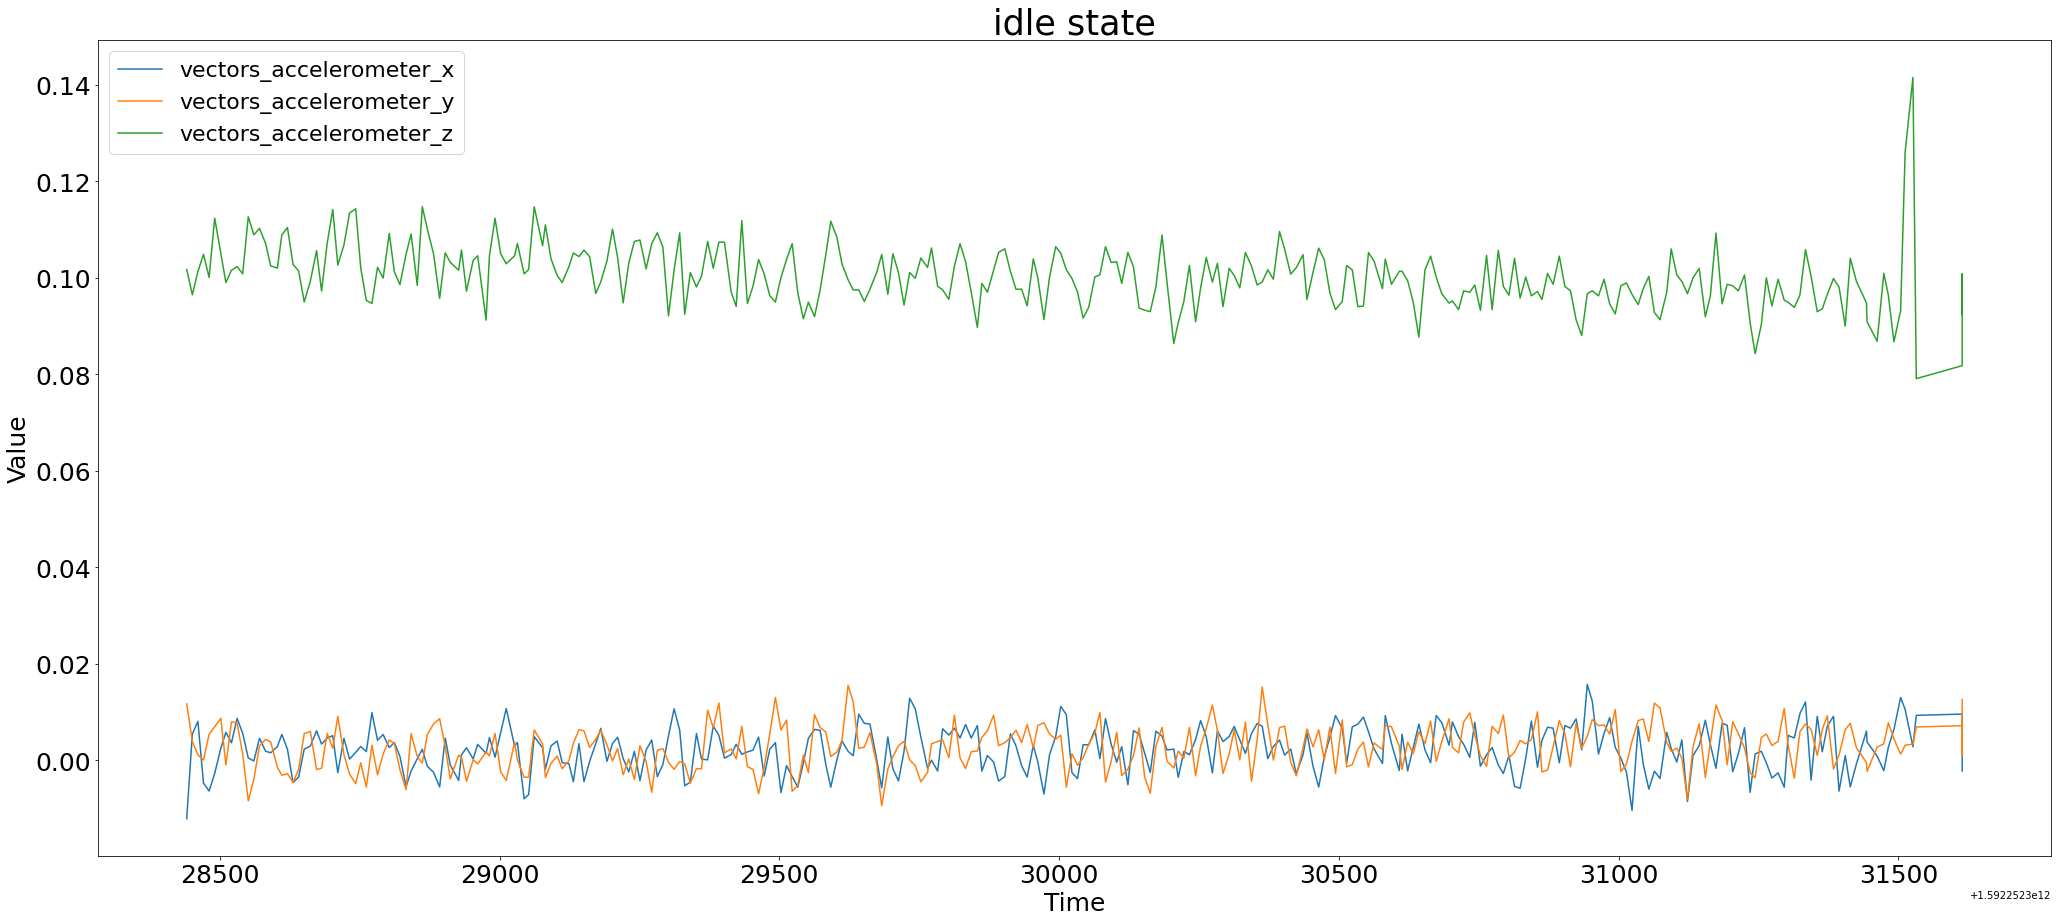
\includegraphics[width=15cm, height=8cm]{idle_state.png}}
    \center{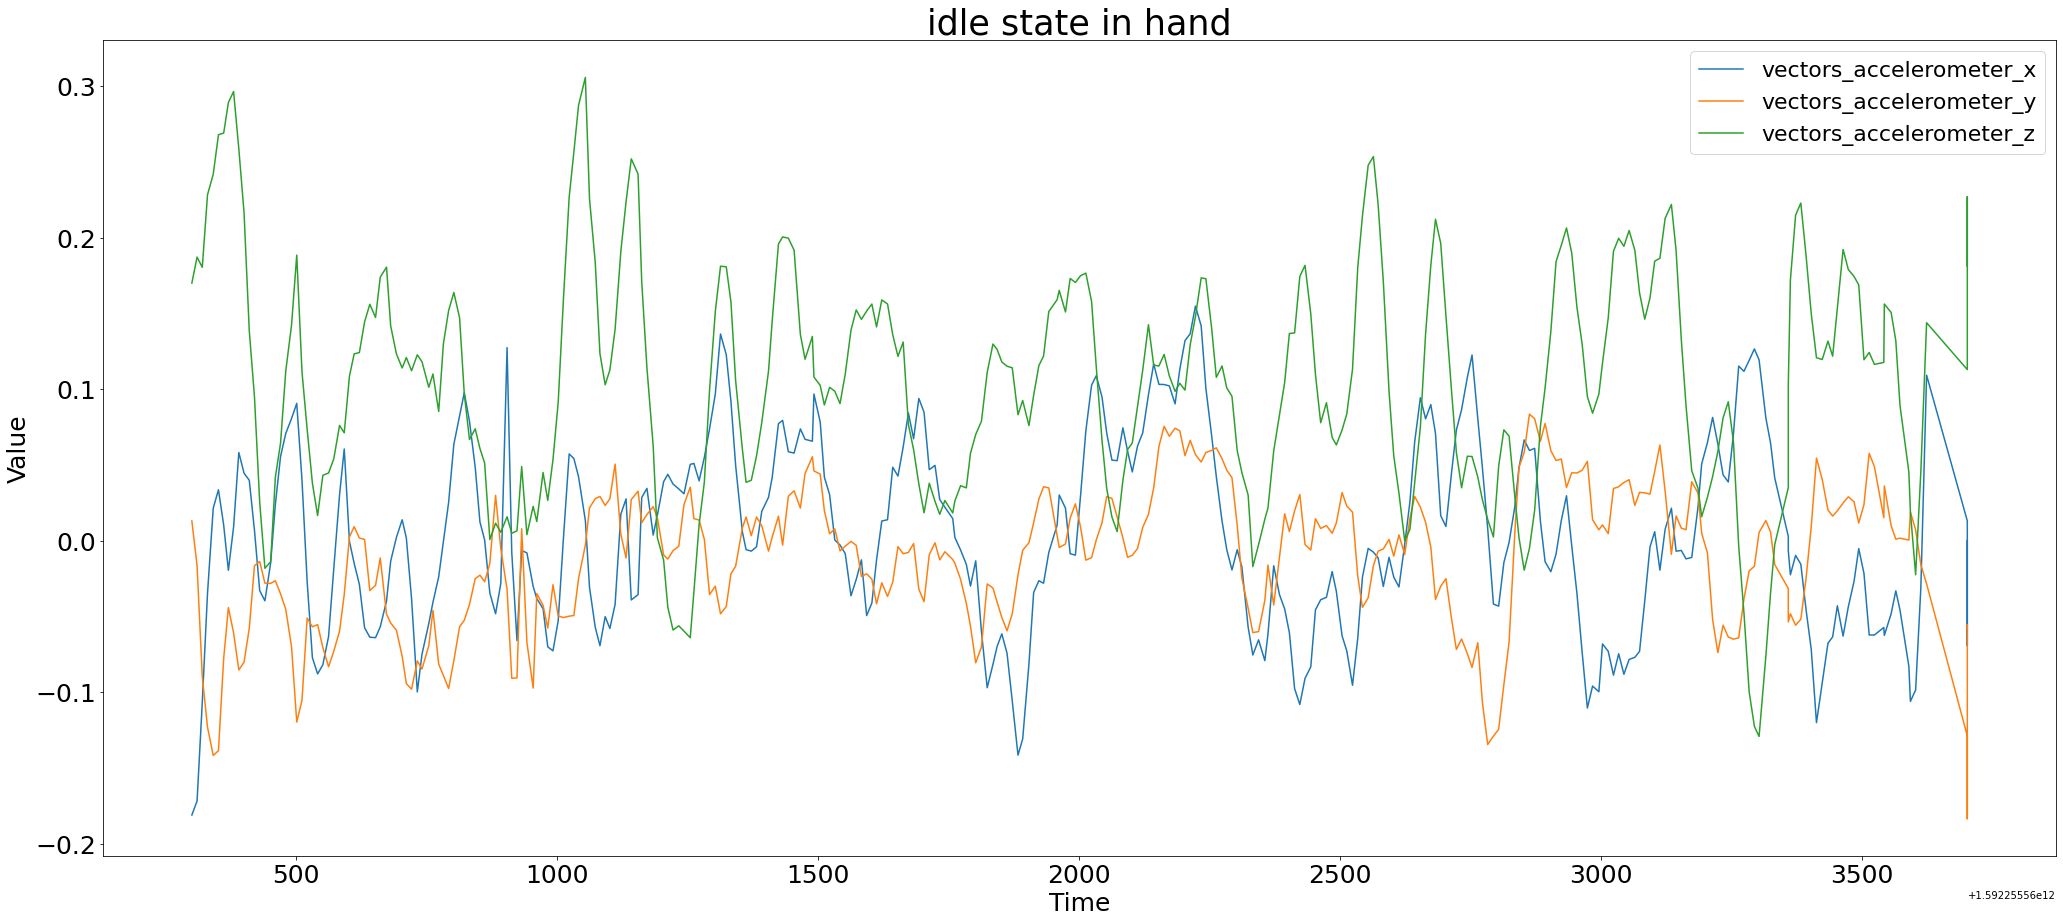
\includegraphics[width=15cm, height=8cm]{idle_state_in_hand.png}}
\end{figure}

\subparagraph{1.} Первый из них показывает значения, которые выдает датчик акселерометра в то время, как телефон находится в неподвижном состоянии (В данном случае видно, что значения не превосходят 0.15).
\subparagraph{2.} Второй показывает значения, которые выдает датчик акселерометра в то время, как телефон находится в состоянии покоя, но уже в руке человека, что дает приблизительно реальные значения данных. (в этом случае получаем, что значения больше в $\sim 2$ раза, чем в 1 эксперименте).
\subparagraph{Итог:}
На данных двух примерах сразу становится видна разница между состоянием бездействия(телефон лежит на столе) и состоянием бездействия(телефон находится в руке), поэтому стоит считать состоянием покоя -- состояние, когда телефон лежит в руке человека. \\
Далее нужно было посмотреть, на сколько сильно меняется жест, при введение такого фильтра (для иллюстрации был использован жест <<Круг>>, состоящего из двух тактов).

\begin{figure}[H]
    \center{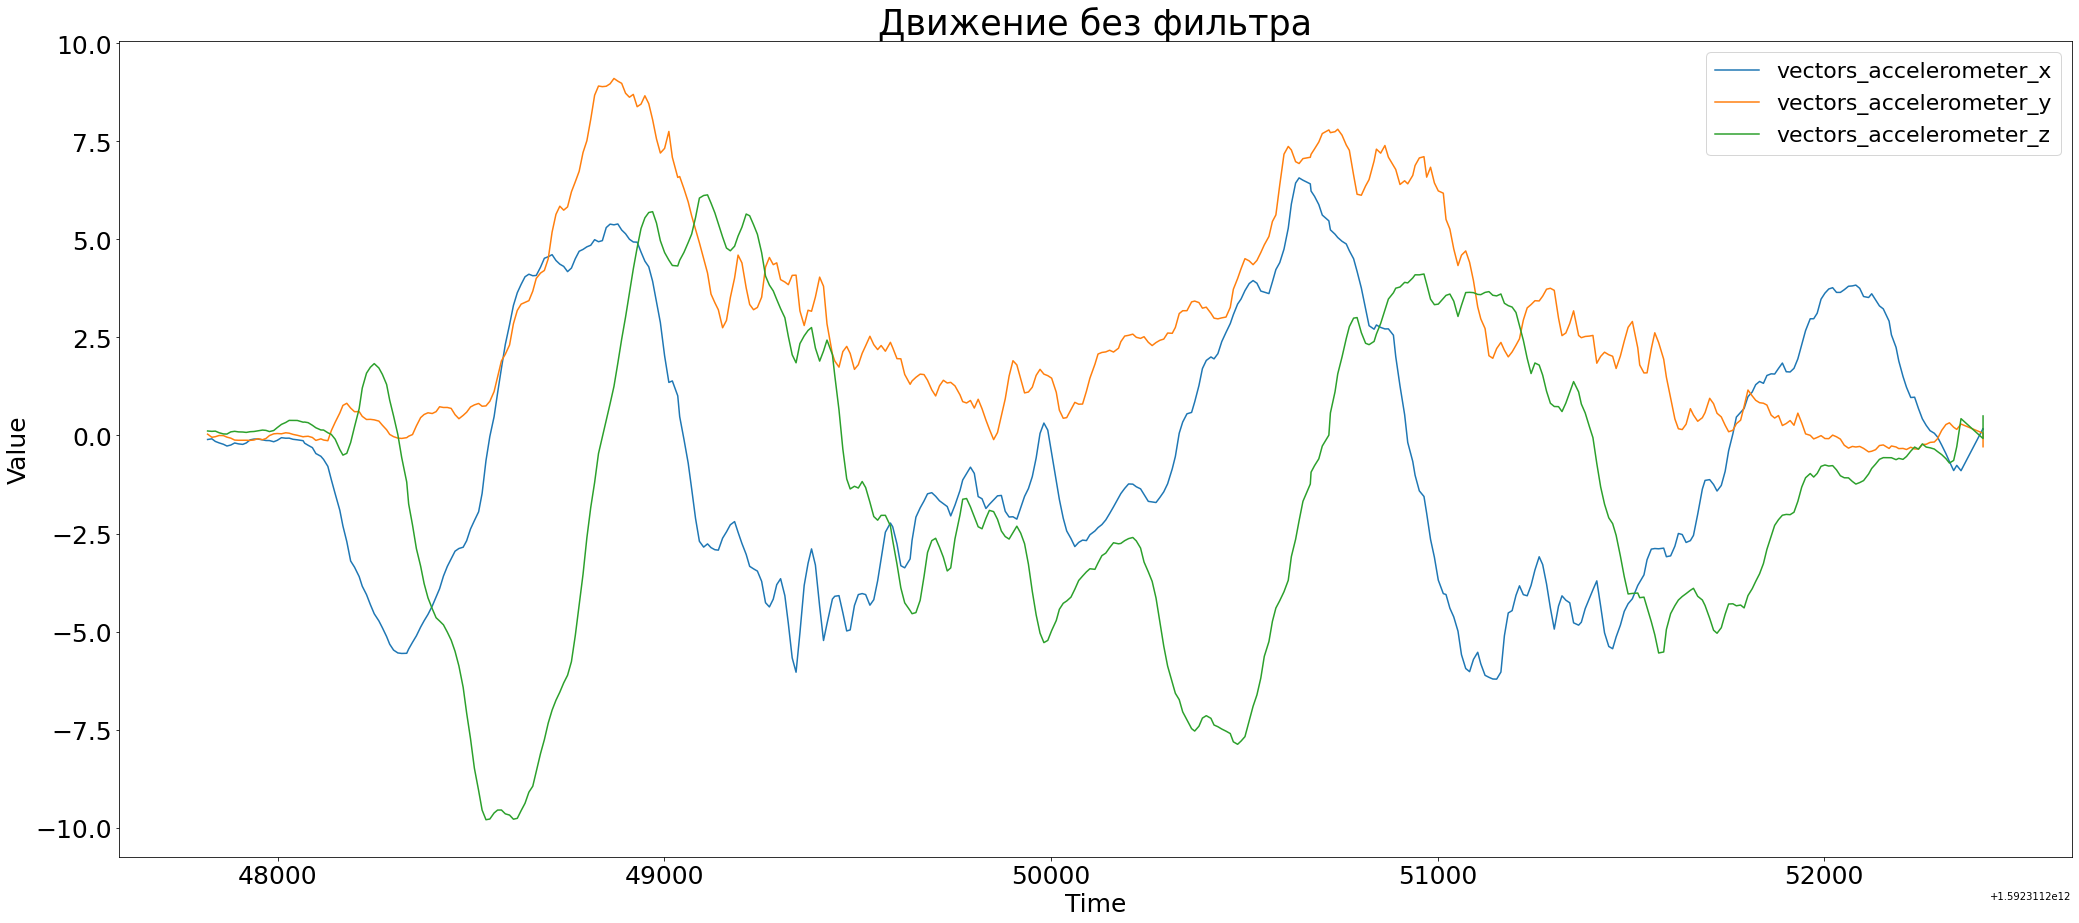
\includegraphics[width=15cm, height=8cm]{gesture_with_no_filter.png}}
    \center{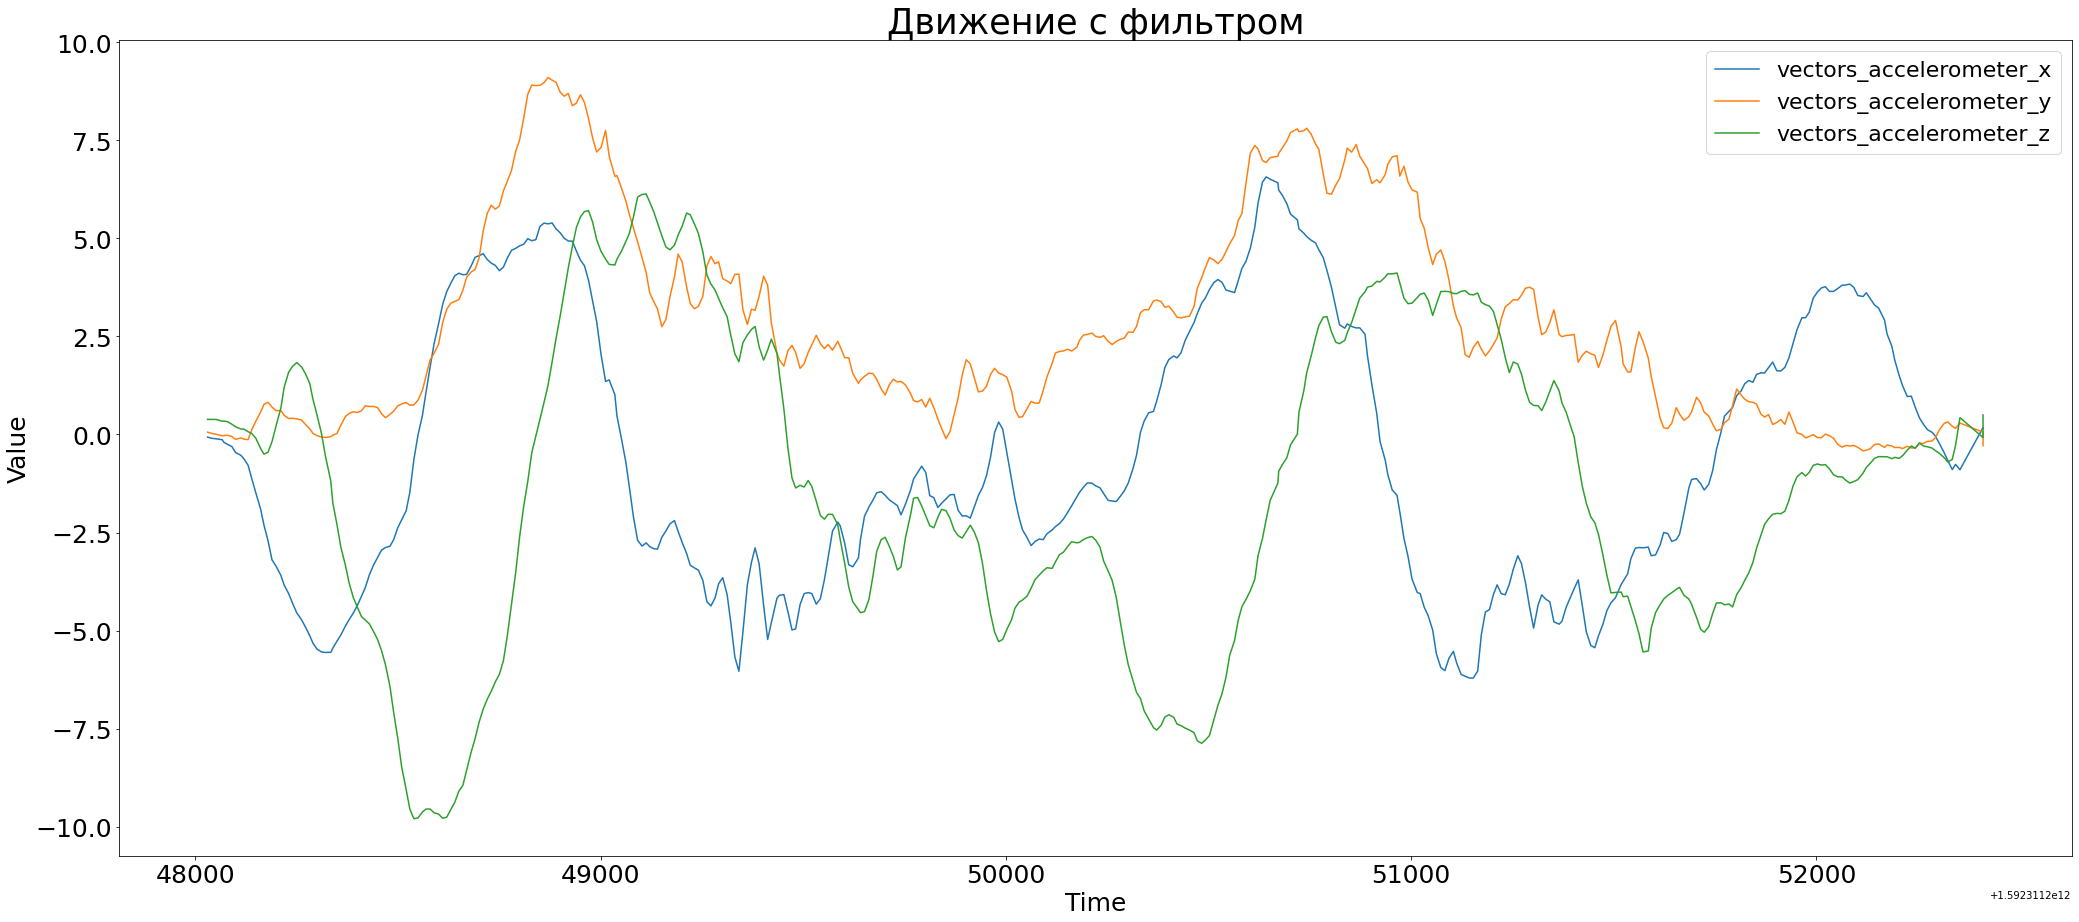
\includegraphics[width=15cm, height=8cm]{gesture_with_filter.png}}
\end{figure}

Сразу можно заметить, что была удалена часть данных из начала, которые соответствовали состонию покоя, что улучшит дальнейший анализ.

\subsubsection*{Автокорреляция:}
Далее для нашего полученного жеста нужно выделить такт, для этого буду использовать корреляцию между двумя случайными величиными, то есть искать какую-то статическую сваимосвзяь между нашими данными: \\
Для начала распишем, что такое ковариация:
\[COV_{XY} = E\left[ (X - E(x)) (Y - E(Y))\right]\]
Так как ковариация будет иметь размерность равную проивзедению размерности случайных величин, то ее не совсем удобно использовать для анализа. И так как в нашем случае у нас дискретные величины (то есть измерение идет с каким-то отчестом (не непрерывно)), то будем использовать корреляцию Пирсона:

Для устранения неудобства использования ковариации был введен линейны коэффицент корреляции (Коэффицент корреляции Пирсоана):
\[r_{XY} = \dfrac{COV_{XY}}{\sigma_x \sigma_Y} = \dfrac{\sum (X - \overline{X}) (Y - \overline{Y})}{ \sqrt{\sum (X - \overline{X})^2 (Y - \overline{Y}) ^2} }; \overline{X} = \dfrac{1}{n} \sum_{i = 1}^n X_i\]
Данная формула записана для коэффицента корреляции по выборке, то есть все математические ожидания заменены на выборочные средние, а диспериии -- на выборочные дисперсии. \\
Такой коэффицент корреляции показыает тесноту линейной взаимосвязи и изменяется в пределах от -1 (полная линейная обратная взаимосвязь) до 1 (полную линейную положительную взаимосвязь).

Для нашей задачи будем использовать функция автокорреляции, которая представляется собой корреляцию Пирсона между исходныи рядом и его версией сдвинутой на несколько отсчетов (на <<лаг>>). $r_i$ -- значение автокореляционной функции с лагом $i$ (от -1 до 1, где 1 -- полное совпадение сигнала, -1 -- обратный сигнал). Вычисляется по следующей формуле:
\[r_i = \dfrac{\sum_{i = lag}^n \left(y_i - \dfrac{\sum_{j = lag}^n y_j}{n - lag} \right) \cdot \left(y_{i-lag} - \dfrac{\sum_{j = lag}^n y_{j - lag}}{n - lag} \right)}{\sqrt{ \left( \sum_{i = lag}^n \left(y_i - \dfrac{\sum_{j = lag}^n y_j}{n - lag} \right)^2 \right) \cdot \left( \sum_{i = lag}^n \left(y_{i - lag} - \dfrac{\sum_{j = lag}^n y_{j-lag}}{n - lag} \right)^2 \right) }}\]
где $y$ -- входной сигнал, $lag$ -- смещение сигнала.

Так как у нас коэффицент корреляции расчитывается по выборке, то получать будем не истинные параметры, а только их оценки, которые каким-либо образом приближаются к реальному параметру. Но для нас это не сильно критично, так как нужно определить количество жестов, которые будут определится по формуле:

$\text{количество тактов} = \dfrac{\text{длина сигнала}}{\text{лучший индекс корреляции}}$, то есть отношение длины сигнала к индексу, на которой корреляция принимает наибольшее значаение.

Теперь нужно данную функцию запрограммировать и посмотреть на полученный результат:

\begin{figure}[H]
    \center{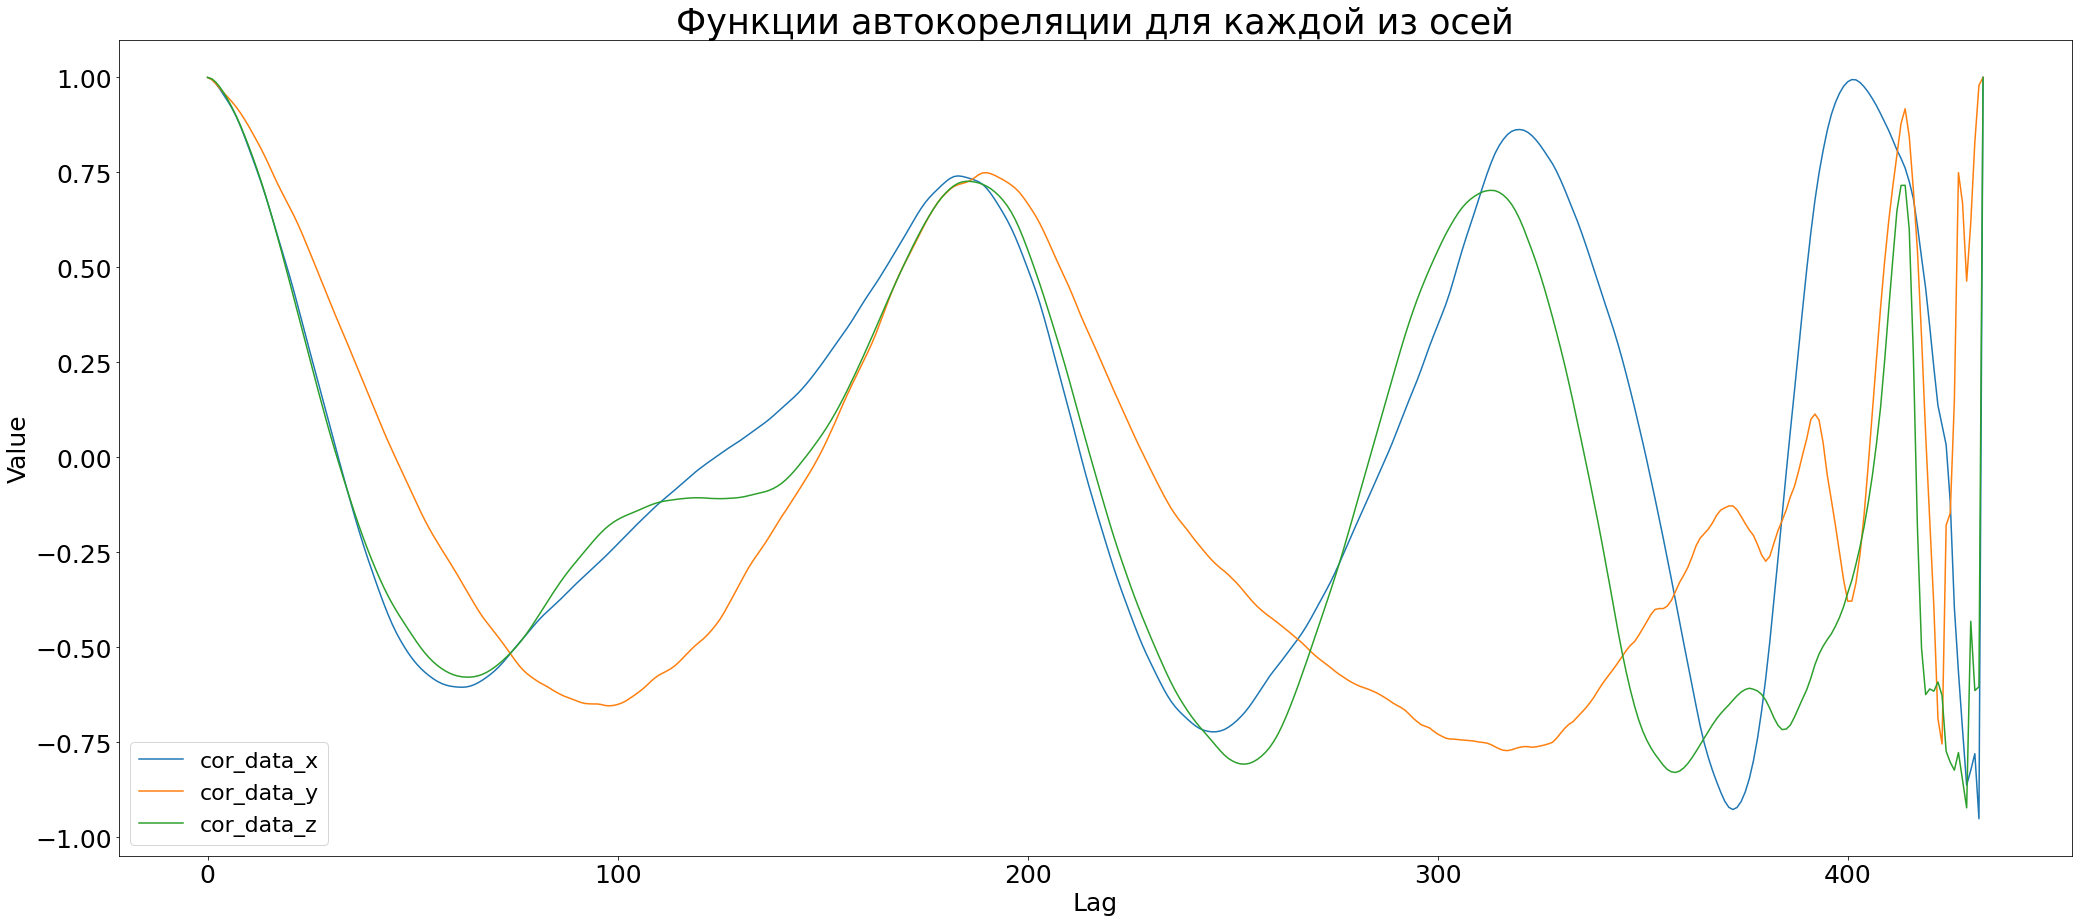
\includegraphics[width=15cm, height=8cm]{cor_data_x_y_z_with_no_delta.png}}
\end{figure}

Как видно, данная функция показывает наиболее значение в самом начале, так из-за маленького количества точек, нельзя достоверно проверить настоящую автокорреляцию, а тажке в конце, так как сигнал полностью совпадает с исходным.
Поэтому стоит не учитывать какое-то количество лагов с начала и конца (путем множественных тестов была выбрана окрестность значения $20 \%$ для первых лагов и $14 \%$ для лагов с конца), поэтому получаем вот такой график:

\begin{figure}[H]
    \center{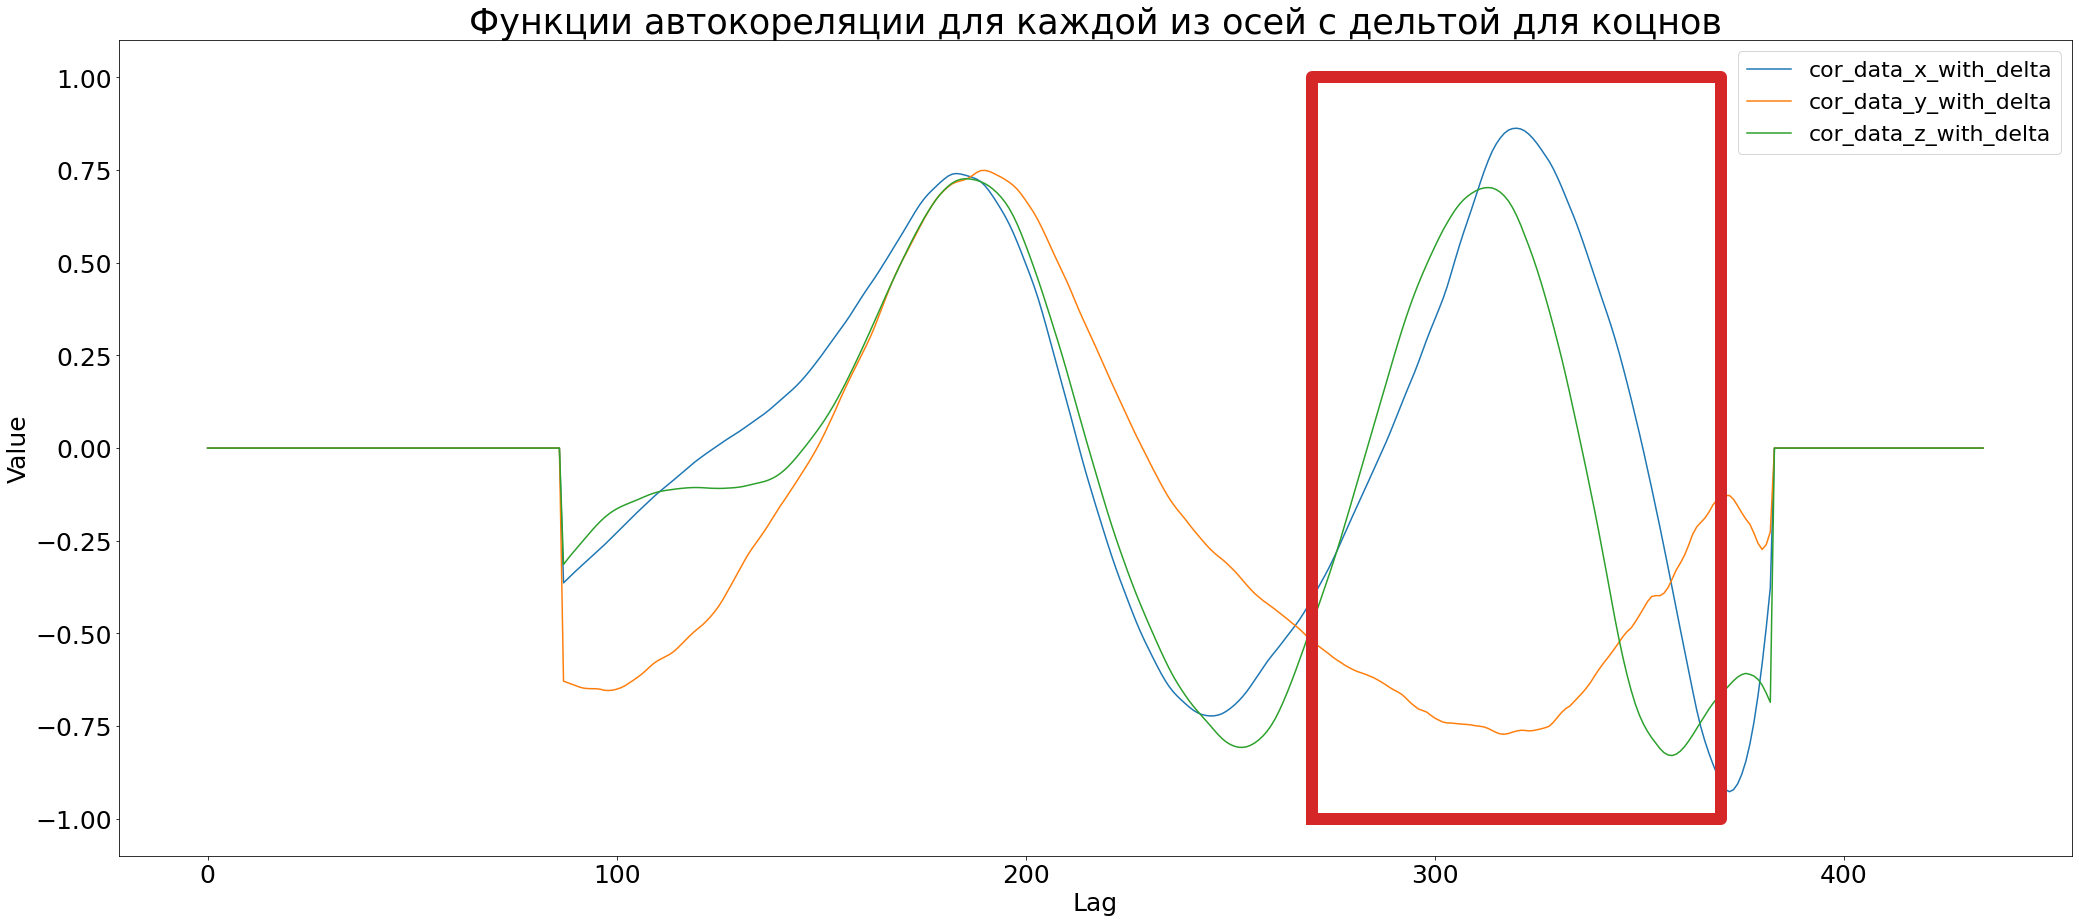
\includegraphics[width=15cm, height=8cm]{cor_data_x_y_z_with_delta.png}}
\end{figure}

И так как задача состояла в распознавании тактов многомерного жеста, а сейчас у нас найдены только функции автокорреляции по отдельным осям. Поэтому нужно как-то связать показатели по каждой из осей к одному показателю: \\
Если же мы будет находить наибольшую корреляцию по каждой из осей, а потом каким-либо образом будем их совмещать, то может получиться такая ситуация, что для одной из осей -- какая-то точка будет являться максимумом, а для другой из осей -- данная точка не будет являться максимумом (Данная ситуация выделена красным квадратом).
Поэтому при поиске наилучшей автокорреляции для многомерного (в нашем случае трехмерного) жеста стоит рассматривать одновременно тройки показателей (по x, по y, по z), и тогда график станет удобным для анализа:

\begin{figure}[H]
    \center{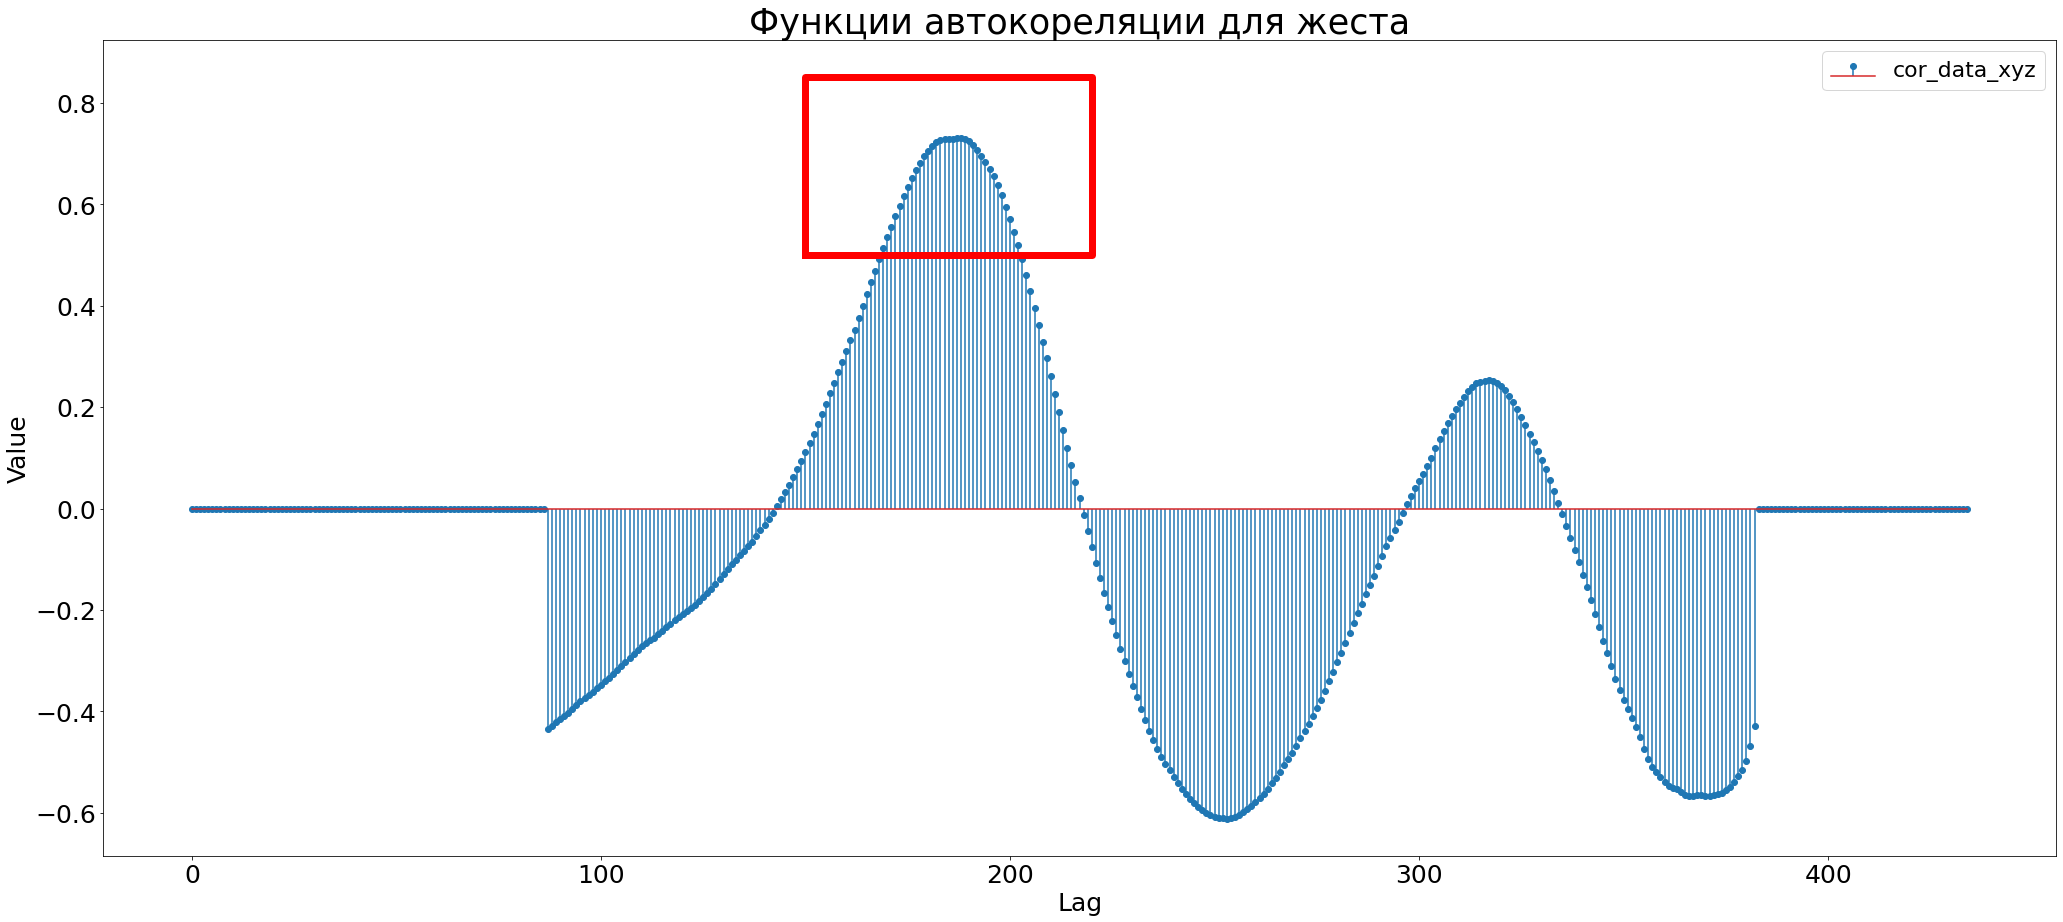
\includegraphics[width=15cm, height=8cm]{cor_data_xyz.png}}
\end{figure}

Как видно, в данном случае решается проблема, возникающая при обработке данных по каждой из осей по отдельности. И сейчас уже легко увидеть самый главную точку, в которй сигналы максимально коррелируются (отмечена на графике).
Для примера был использован жест "Круг", состоящий из двух тактов.
И на данный момент задача кажется уже решенной, тогда остается только написать часть кода, находящей индекс, на котором фунция автокорреляции принимала бы наибольшее значение.
Но на самом деле был не учтен еще один факт: две или более части сигнала могут коррелировать схожим образом, если мы будеи изображать замкнутые фигуры, состоящие из нескольких тактов, например, рассмотрим жест "Круг", состоящий из 3 тактов: (картинка находится чуть ниже)

\begin{figure}[H]
    \center{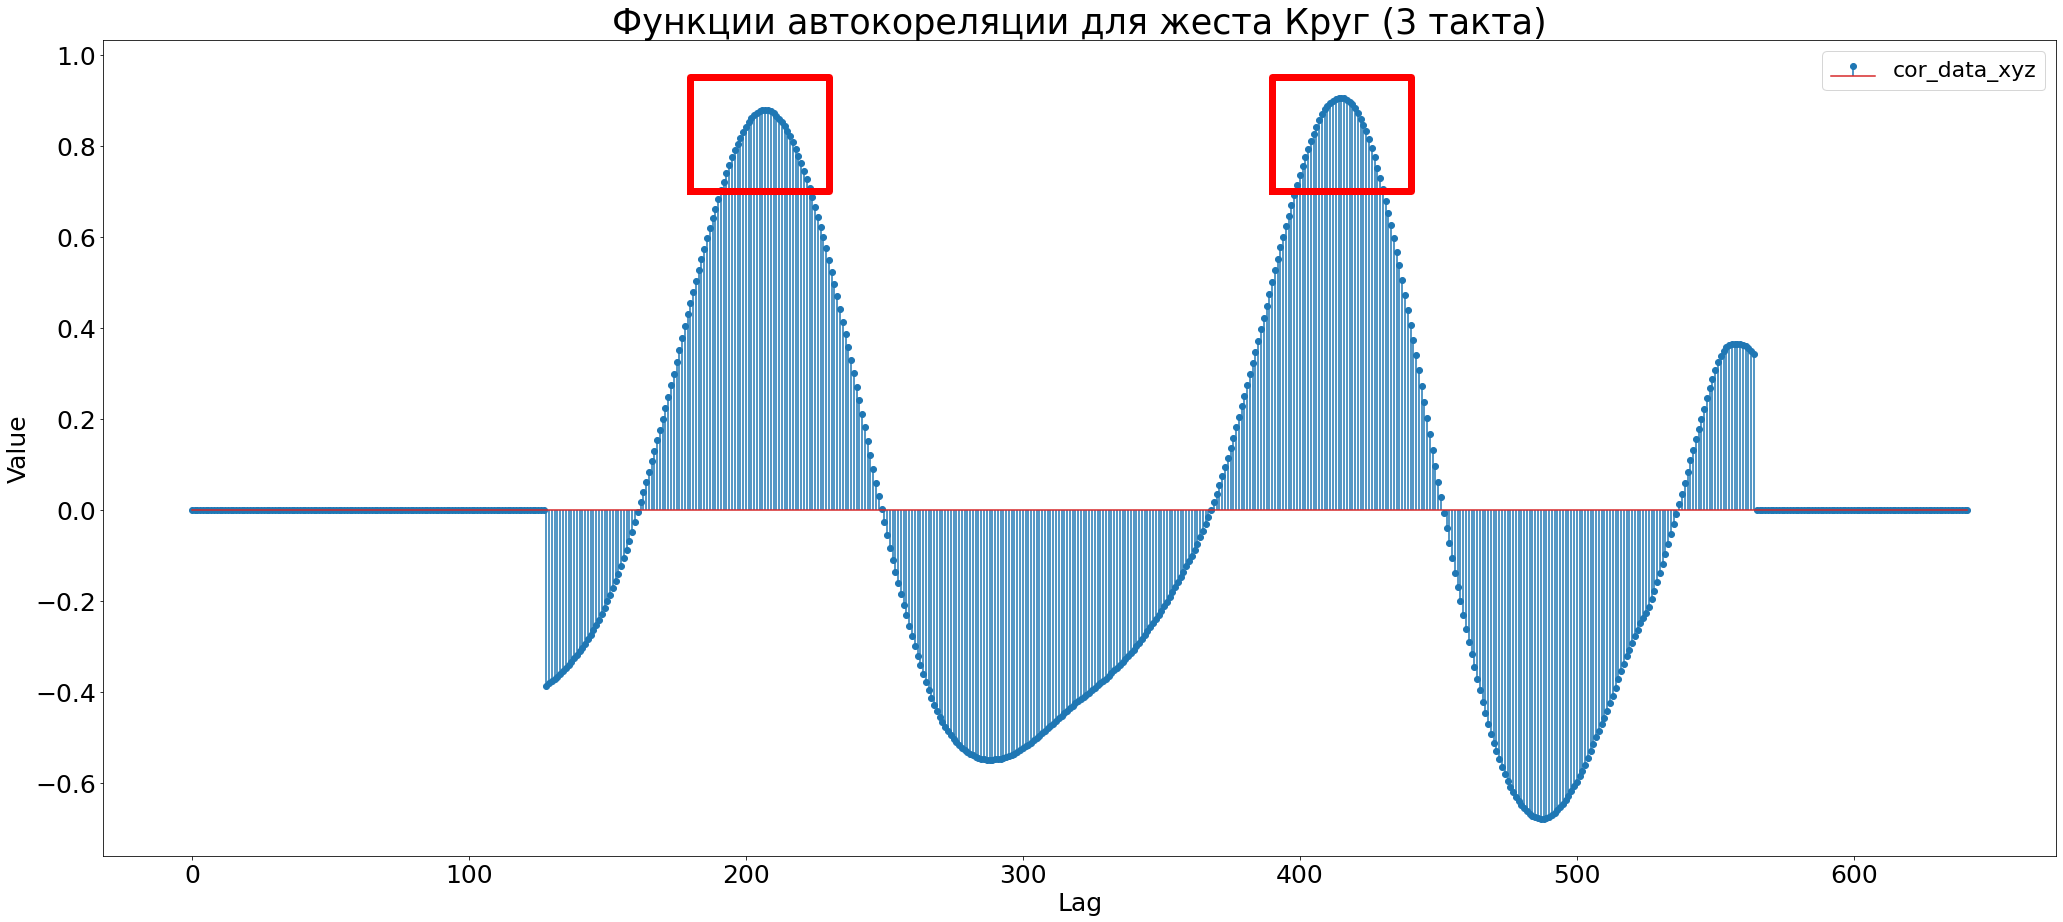
\includegraphics[width=15cm, height=8cm]{cor_data_xyz_3_circle.png}}
\end{figure}

Для решения такой проблемы (выделена краснымии крвадратами на графике) будет делать слудущее:

будеи искать наибольшее значение в первой "волне" и считать его за наиболее коррелируемым с нашими входящими данными. \\
Если же мы найдем значени автокорреляции, большее чем уже существующий максимум, то такую точку будем считать новым максимумом только в случае, если она больше текущего максимума на определенный процент (который был вычислен путем множества тестов $\sim 22 \%$) от существующего максима (данное решение будет работать, так как корреляции в таких точках будут отличаться друг от друга на небольшой процент, что не повлияет на общее выделение правильного такта).

А также было принято решение не рассматривать разбиение жеста на такты, если его наибольшая корреляция составляет менее 0.33 (обосновывается тем, что ряд плохо коррелируем со всеми своими копиями, свдинутыми на всевозможные лаги, что говорит об отстутствии цикличности).

\subsubsection*{Усреднение движения:}
После того, как был найден индекс массива, при котором достигается наибольшая корреляция, нужно посчитать количество тактов в нашем жесте и усреднить все такты, чтобы получился единый жест, состояший из одного такта движения.

\subparagraph*{Реальное количество жестов:}
Как уже упоминалось ранее, функция автокорреляции будет выдавать лишь оценку на реальный параметр, поэтому для избежания неправильного определния количествао тактов, будем пользоваться формулой:
\[\text{количество тактов} = \dfrac{\text{длина сигнала}}{\text{лучший индекс корреляции}}\]
Данная формула будет выдавать не точные значения, а числа, записанные в десятичной форме, в данном случае будем применять арифметическое округление, которое в среднем будет давать правильную оценку на количество тактов в нашем движении.
\subparagraph*{Усреднение жестов:}
Так как в самом начале был убрано влияние на жест состояния покоя до и после жеста, то можео считать, что сейчас в данных находятся только сами такты движений, при этом делаем предположение, что все такты сделаны с одной скоростью, тогда $i$-ая точка любого жеста по любой из осей будет высчитываться по следующей формуле:
\[x_i = \dfrac{\sum_{j = 1}^{\text{количество тактов}} x_{i + \text{количество тактов} \cdot j}}{\text{количество тактов}}\]
Проделав такую операцию со всеми точками такта, можно получить итоговый (усреденный) такт одного жеста:

\begin{figure}[H]
    \center{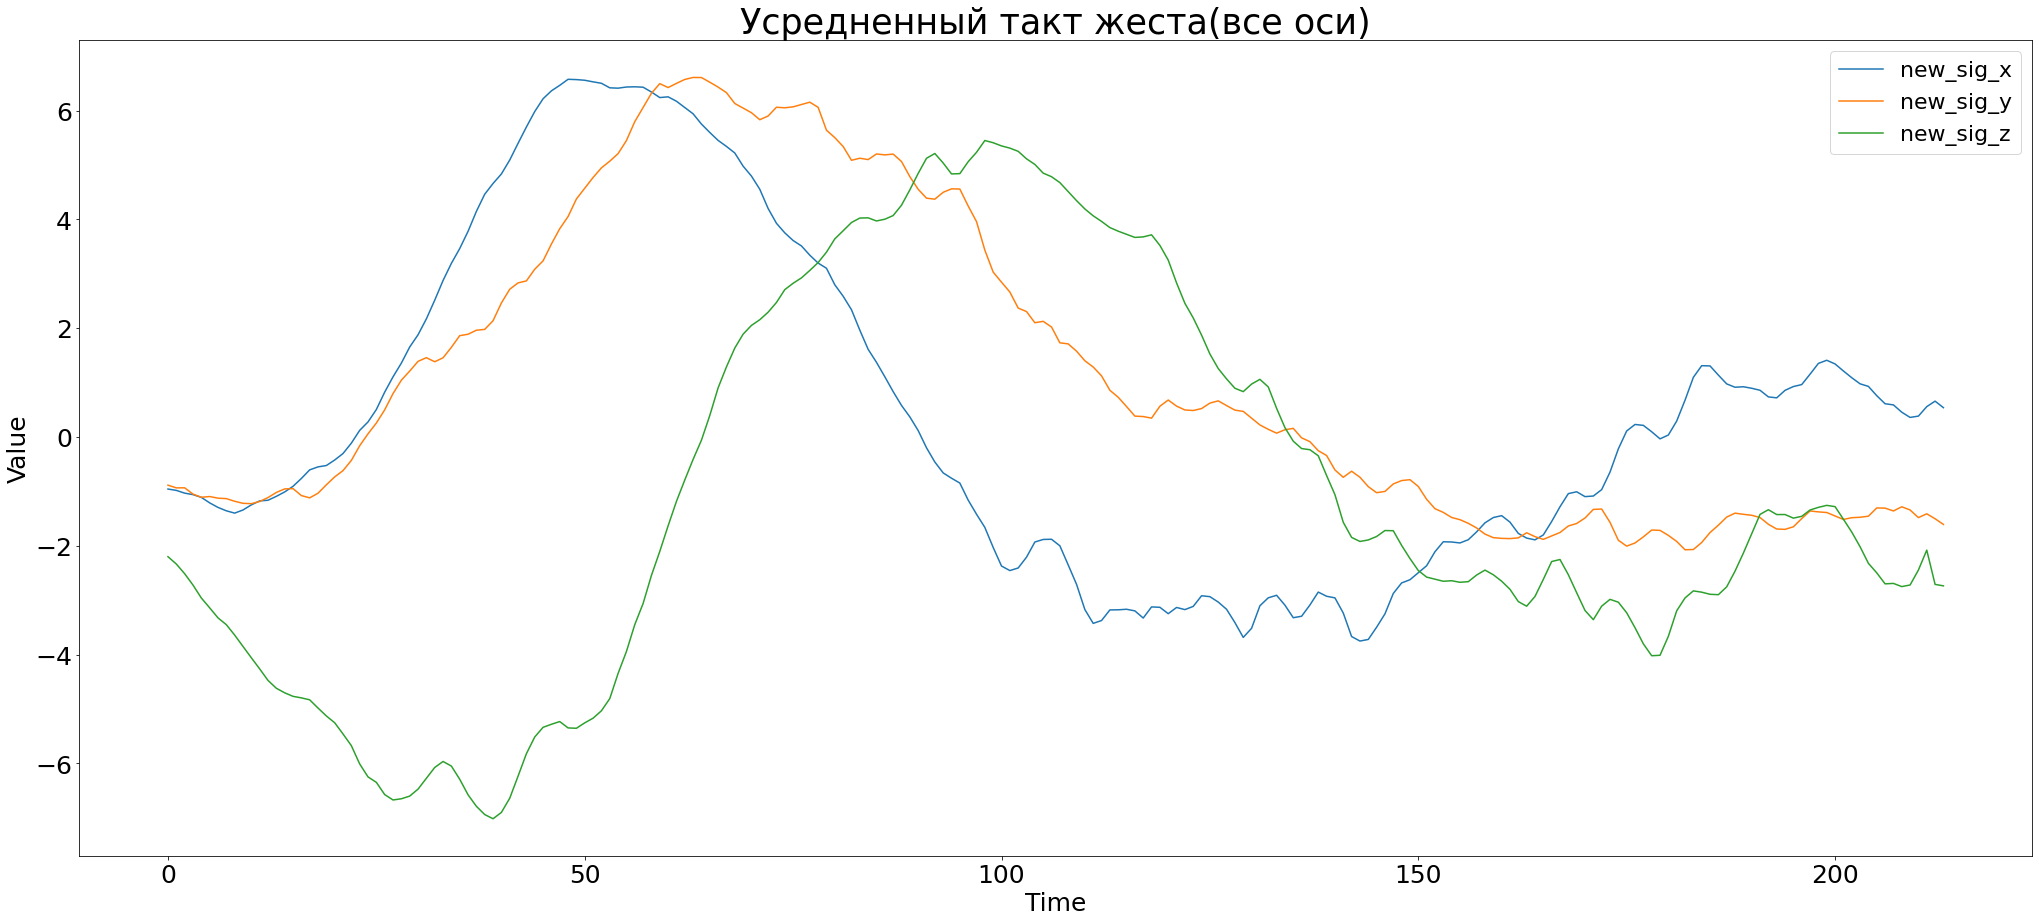
\includegraphics[width=15cm, height=8cm]{avr_gesture.png}}
\end{figure}

Далее полученные данные отправляются на обработку другим членам команды.

\subsection*{Описание вычислительного эксперимента – план эксперимента, инструменты и средства его проведения, полученные результаты, их анализ и оценка.}
После проделанной тоеретической части, остается объеденить все запрограммированные функции в одну, которая должна принмать три массива данных (данные с акселерометра по трем осям), и должна выдавать новые усредненные данные по трем осям.

Далее нужно записать большое количество жестов с разным количетсвом тактов для проверки работоспособности алгоритма:
Например, вот результаты работы тестирующей программы для одного из жестов:
(программа на вход принимает директорию, в которой расположены файлы, при этом их названия должны быть в таком формате: $x\_*.json$, где $x$ -- число тактов в записанном движении, далее программа запускает все описанные выше функции и сравнивает результат работы функций(те выделенное количество тактов) с заявленным числом $x$. После чего подводится статистика по заданной директиории)

\begin{figure}[H]
    \center{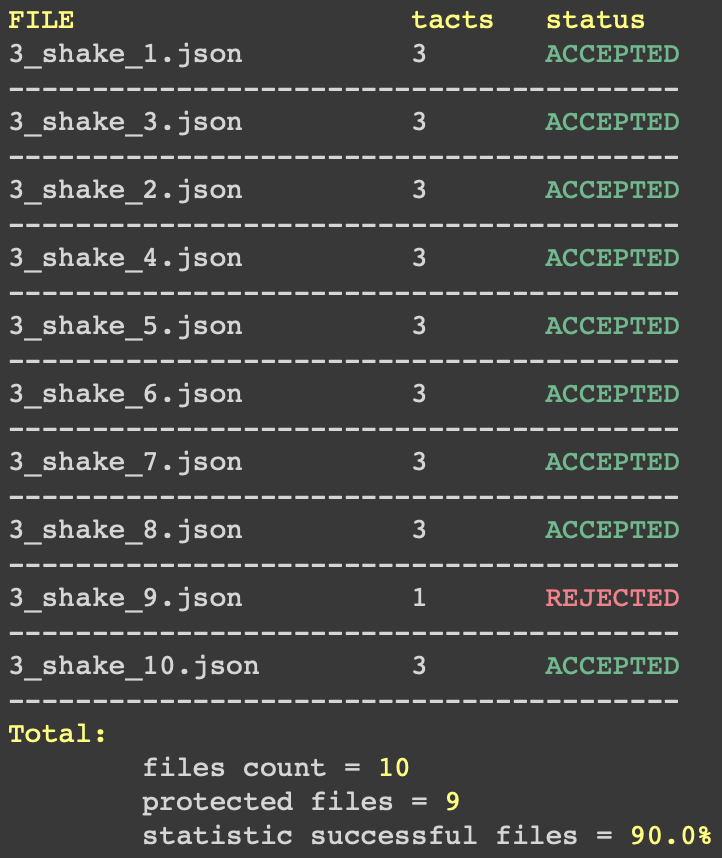
\includegraphics[scale = 0.5]{example_of_test_part.png}}
\end{figure}

После проведения таких тестов по всем жестам, которые мы будет распознавать, получаем следующую диаграмму с результатами тестов: \\

\begin{figure}[H]
    \center{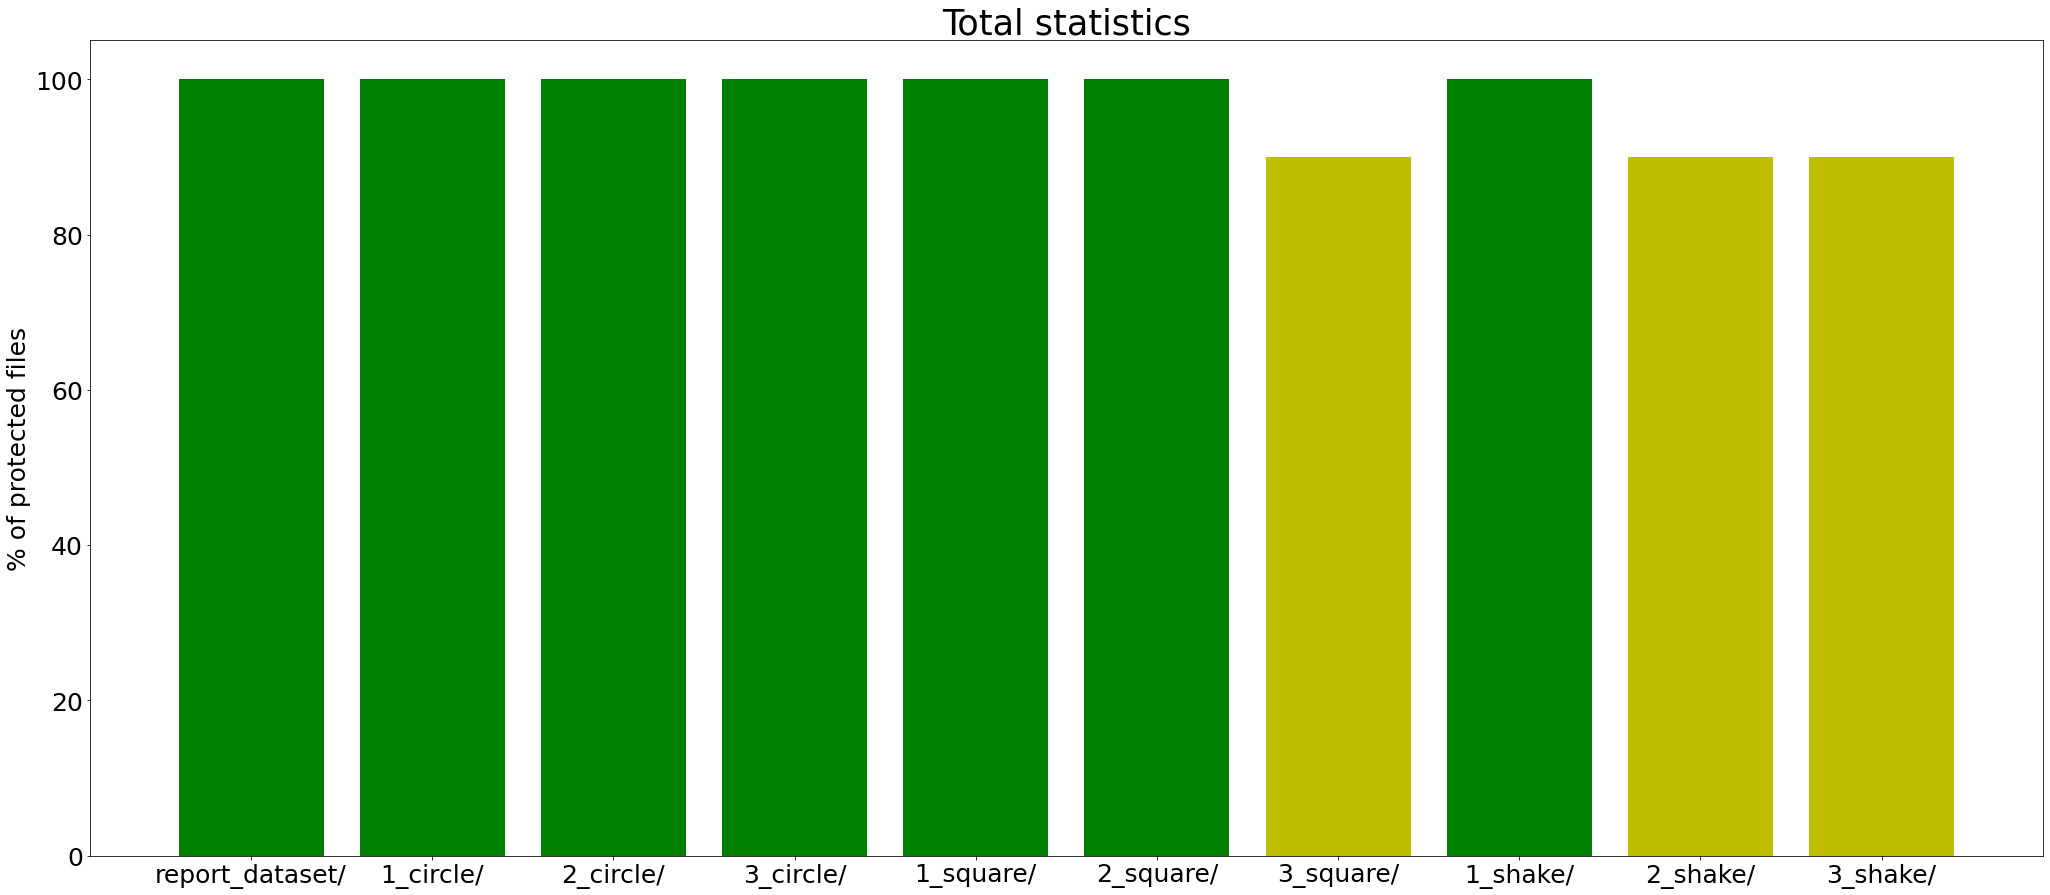
\includegraphics[width=15cm, height=8cm]{total_statistics.png}}
\end{figure}

Также, в ходе всех тестирований были более детально подобраны все параметры, описанные ранее, для максимизации правильности опреедления тактов.

Как видно, почти все жесты распознаются с максимальной веротяностью, кроме трех из них (3 круга, 2 встряхивания, 3 встряхивания) и вероятности ошибок распредпелны равномерно:

\begin{figure}[H]
    \center{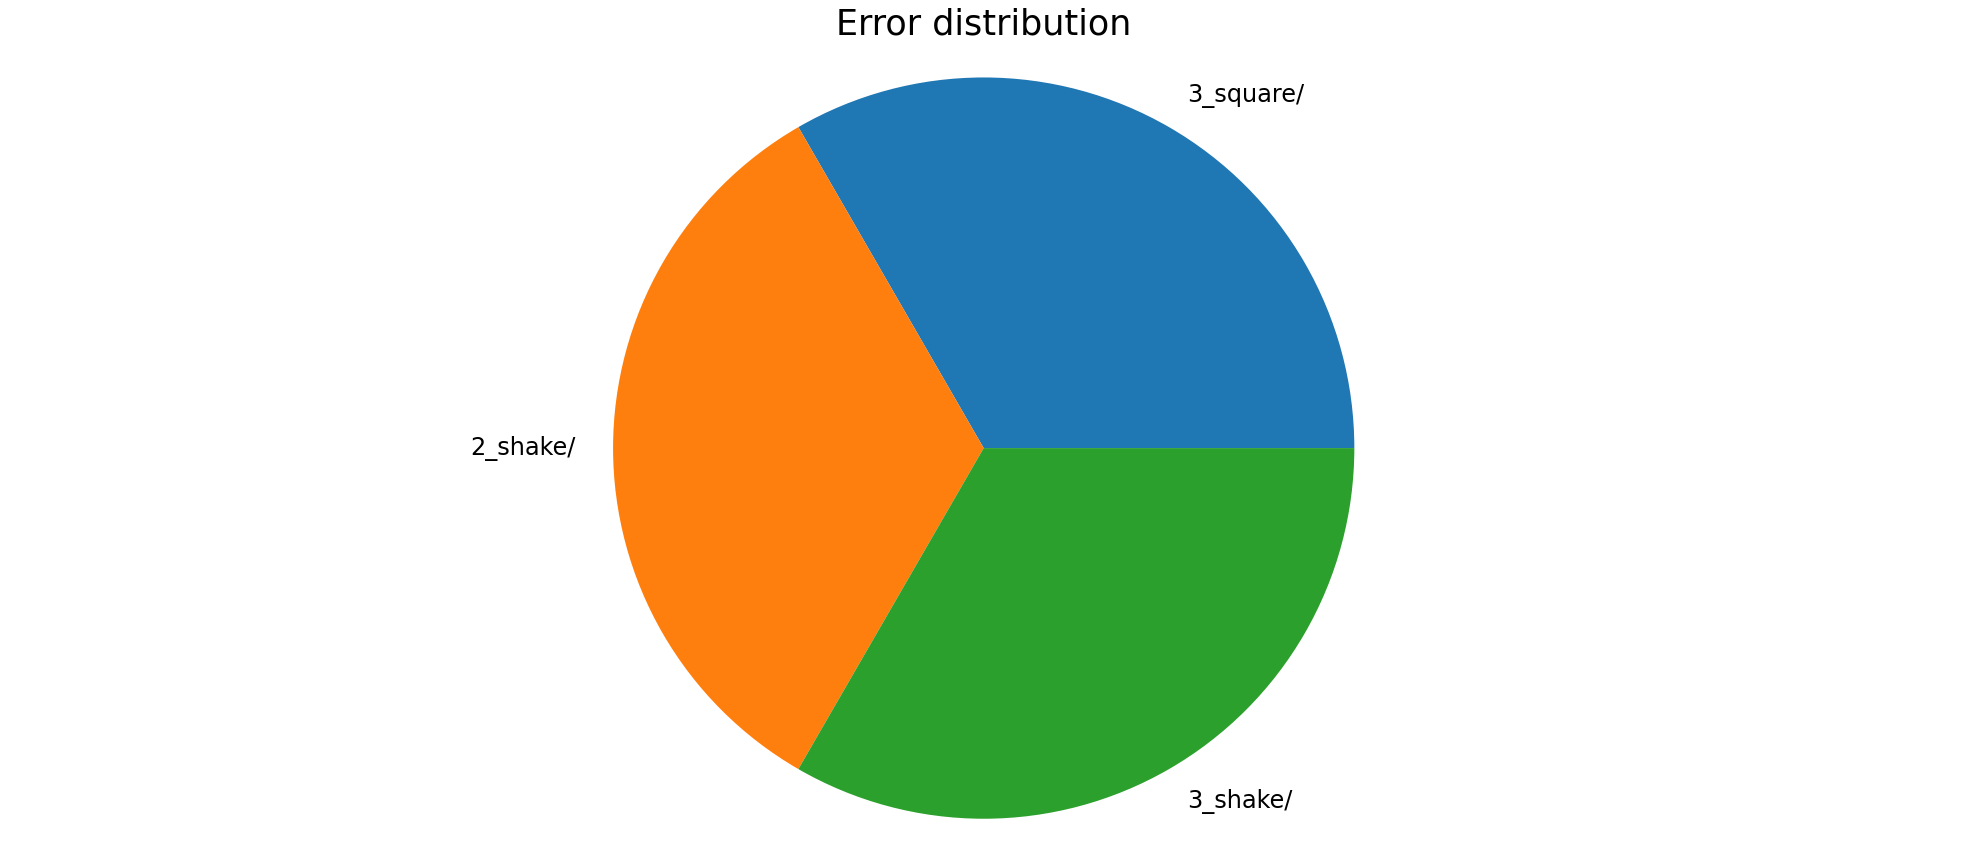
\includegraphics[scale = 0.22]{error_distribution.png}}
\end{figure}


Следовательно, данное тестирование показало правильность выбора алгоритма по распознванию тактов многомерного жеста.

\section*{Часть Самарина Артема}

\subsection*{Теоретическая часть}
Моей главной задачей было научиться восстанавливать движения телефона по имеющимся у нас данным – времени, показателям акселерометра и гироскопа.

\subsubsection*{НЕУДАЧНЫЙ СПОСОБ}

Для начала задача решалась самым прямым образом - данные аксселерометра (т.е. ускорение по каждой из осей телефона) дважды интегрировались и таким образом получалаось положение телефона в каждый момент времени, но из=за большой погрешности, двойного интегрирования и помех ничего не вышло – картинка съезжала и вместо допустим нужного квадрата получалась спираль. Изначально, я это списывал на то, что акселерометр учитывает ускорение свободного падения, но это оказалось не так.

\subsubsection*{С ЧЕМ ВООБЩЕ РАБОТАЕМ?}

На вход я получаю массив с 7-ю параметрами: время от начала движения, ускорение по оси X, ускорение по оси Y, ускорение по оси Z, угол поворта по X (Pitch), угол поворота по Y (Roll) и угол поворота по Z (Yaw).

\begin{figure}[H]
    \center{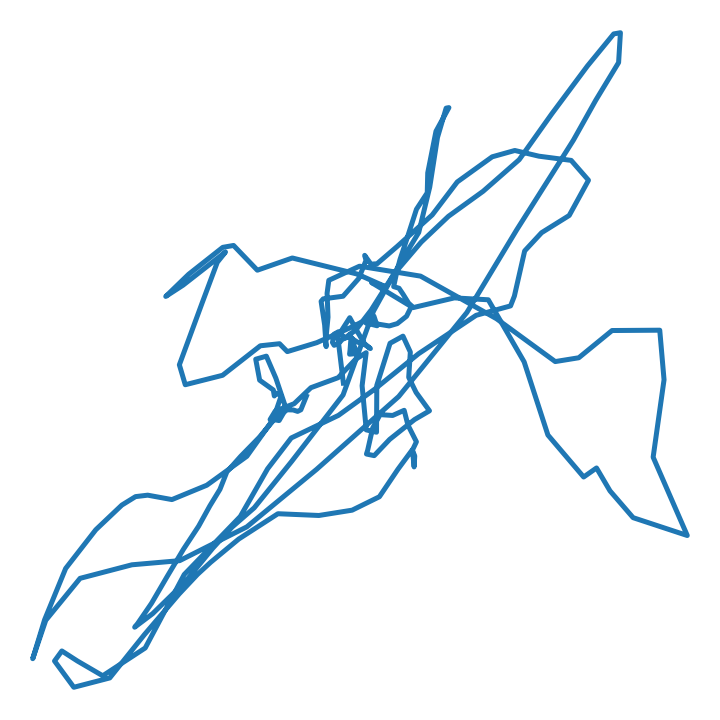
\includegraphics[scale = 0.7]{1.png}}
\end{figure}

\subsubsection*{НОРМАЛИЗАЦИЯ ДАННЫХ}
Для своей задачи я использую 2 фильтра – тот что реализован другим членом моей команды и свой. Мой фильтр сглаживает определенную погрешность. 

\begin{figure}[H]
    \center{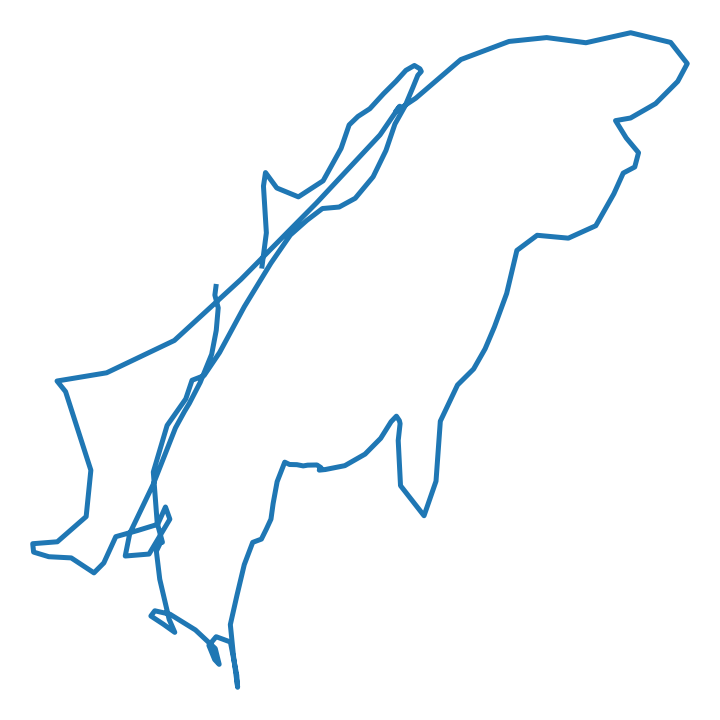
\includegraphics[scale = 0.7]{2.png}}
\end{figure}

А так же из каждого значения акселерометра по каждой оси вычитается среднее по это оси.

\begin{figure}[H]
    \center{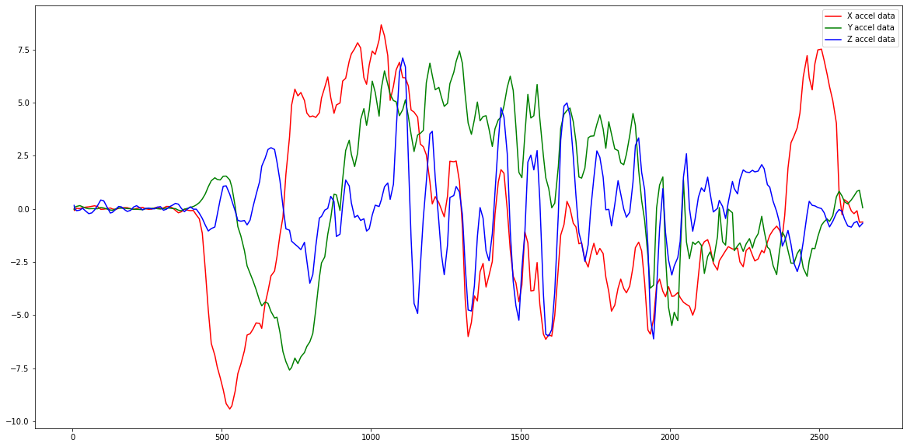
\includegraphics[scale = 0.85]{graph_1.png}}
    \center{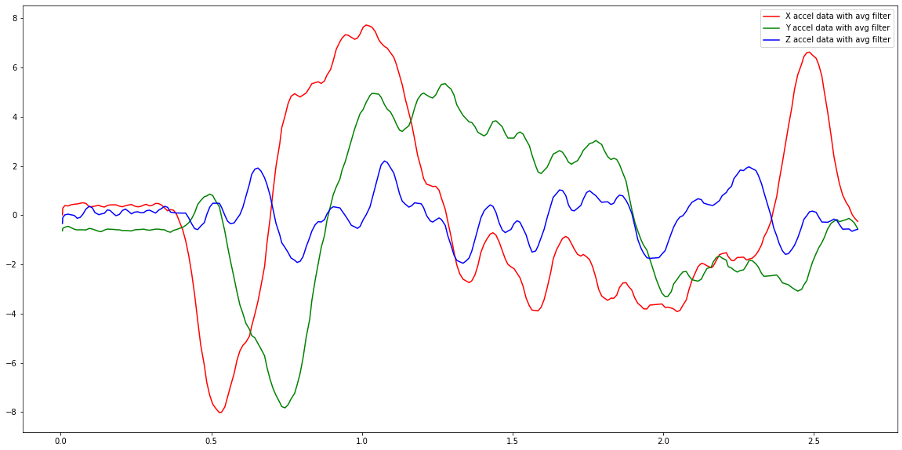
\includegraphics[scale = 0.85]{graph_2.png}}
\end{figure}

\subsubsection*{НАХОЖДЕНИЕ ПОЛОЖЕНИЯ ТЕЛЕФОНА БЕЗ УЧЕТА ДАННЫХ ИЗ ГИРОСКОПА}

После того как данные нормализованы – как уже говорилось ранее – данные акселерометра дважды интегрируются. Если данные акселерометра по X – это вектор А, а время – это вектор T, то положение в каждый момент времени определяется, как $A[i] * (T[i] - T[i-1])$.

\begin{figure}[H]
    \center{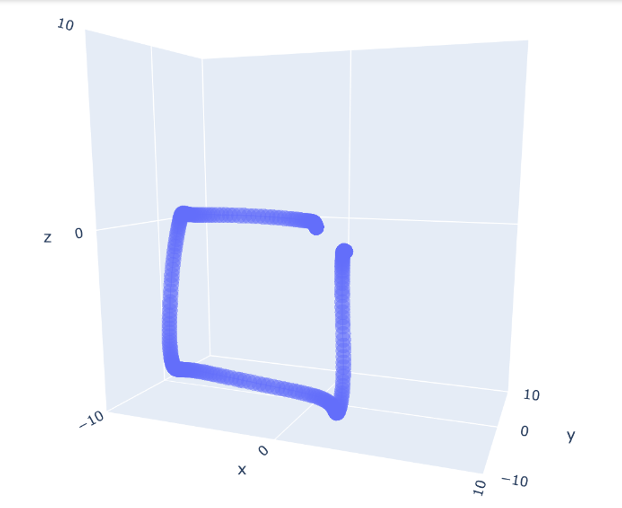
\includegraphics[scale = 0.85]{3d_graph_1.png}}
    \center{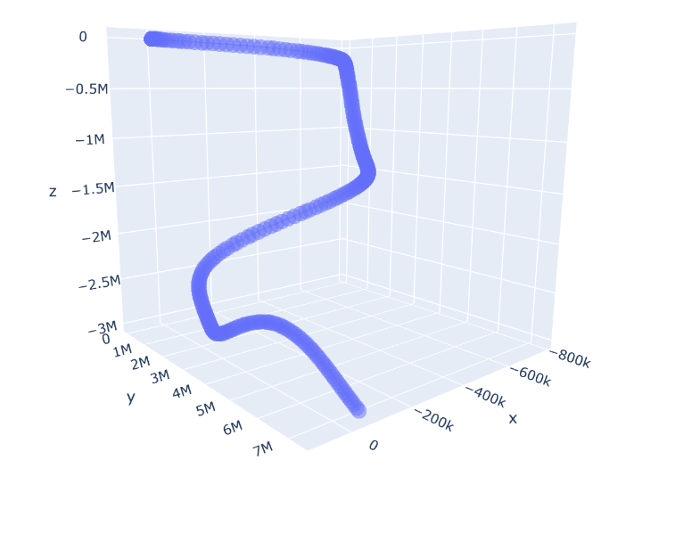
\includegraphics[scale = 0.85]{3d_graph_2.png}}
\end{figure}

\subsubsection*{ПОЧЕМУ И КАК ЭТО РАБОТАЕТ?}

Когда человек рисует жест (а это основной смысл разрабатываемой нами технологии), то он стоит на месте и телефон, как правило, держит в одном положении, просто потому что это удобно – телефоны широкие и как либо менять угол его поворота сложно, если не делать это намеренно. Соответственно, если угол поворота телефона меняется, то хорошее отображение движения телефона не получится.

\subsubsection*{КАК И ЗАЧЕМ УЧИТЫВАТЬ ДАННЫЕ ГИРОСКОПА?}

Данные гироскопа учитываются для того, чтобы компенсировать угол вращения телефона. Если учитывать угол поворота, то можно получить положение телефона относительно земли, а не относительно движения вдоль своих осей.
Для этого берется вектор значений гироскопа в момент времени 0 и умножается на эту матрицу (затехайте пожалуйста matrix [[ cos(z)*cos(y), -sin(z)*cos(x) + cos(z)*sin(x)*sin(y), sin(z)*sin(x)+ cos(x)*cos(z)*sin(y)], [cos(z)*cos(y), cos(z)*cos(x) + sin(x)*sin(y), -cos(z)*sin(x)+ cos(x)*sin(z)*sin(y)], [-sin(y), cos(y)*sin(x), cos(x)*cos(y)]]) и получается угол поворота в следующий момент времени относительно земли. Зная эти углы, мы можем компенсировать движение телефона вокруг своих осей и находить более точное положение телефона в пространстве.

\begin{equation*}
    \begin{pmatrix}
        cos(z)*cos(y) & -sin(z)*cos(x) + cos(z)*sin(x)*sin(y) & sin(z)*sin(x)+ cos(x)*cos(z)*sin(y) \\
        cos(z)*cos(y) & cos(z)*cos(x) + sin(x)*sin(y) & -cos(z)*sin(x)+ cos(x)*sin(z)*sin(y) \\
        -sin(y) & cos(y)*sin(x) & cos(x)*cos(y) \\
    \end{pmatrix}
\end{equation*}
и получается угол поворота в следующий момент времени относительно земли. Зная эти углы, мы можем компенсировать движение телефона вокруг своих осей и находить более точное положение телефона в пространстве.


\subsection{Разработка метода поиска наилучшей плоскости для проекции (Савосин Артем)}

На вход подаются пред обработанные данные - отфильтрованные, усредненные по тактам (если их было несколько). Данные задаются массивом из 3-х мерных векторов, которые выглядят вот так
\begin{figure}[H]
\center{
\includegraphics[scale = 0.5]{images_sav/3d_fig.png}}
\end{figure}
Для наших данных хотим найти такую двумерную плоскость, что на ней отобразится максимум информации про наше движение - минимум точек совпадут с друг с другом и 2d картинка останется максимально похожей на свой 3d аналог. 

Уравнение плоскости задается уравнением $ax+by+c=z$. 
Задаем систему уравнений 
\begin{figure}[H]
\center{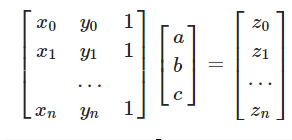
\includegraphics[scale = 1]{images_sav/math1.png}}
\end{figure}
где $(x_i, y_i, z_i)$  - это векторы из массива, а (a, b, c) - нормаль, которую нам нужно найти. В силу того, что в массиве у нас явно больше, чем 3 вектора, система будет переполненной, и нам нужно будет использовать псевдообратную матрицу 
\begin{figure}[H]
\center{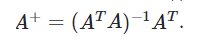
\includegraphics[scale = 1]{images_sav/math2.png}}
\end{figure}
Таким образом нормаль плоскости находится по формуле
\begin{figure}[H]
\center{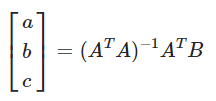
\includegraphics[scale = 1]{images_sav/math3.png}}
\end{figure}
\begin{figure}[H]
\center{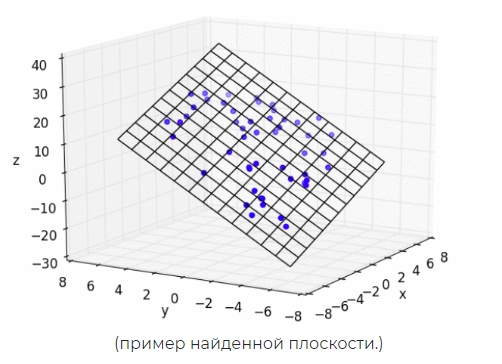
\includegraphics[scale = 1]{images_sav/flat_plot.png}}
\end{figure}
Таким образом мы нашли нормаль для подходящей плоскости. Теперь остается только стандартным способом найти проекцию всех точек на эту плоскость и получить плоскую картинку движения.
\begin{figure}[H]
\center{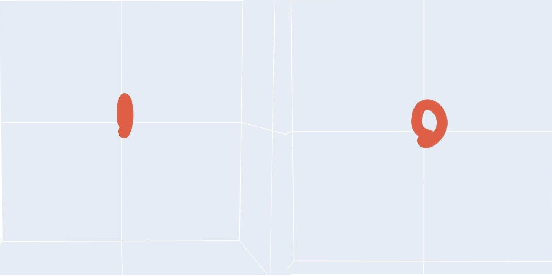
\includegraphics[scale = 1]{images_sav/2d_fig.png}}
\end{figure}
Получилась плоская фигура, находящаяся в 3D пространстве, из нее получаем 2D изображение.
\begin{figure}[H]
\center{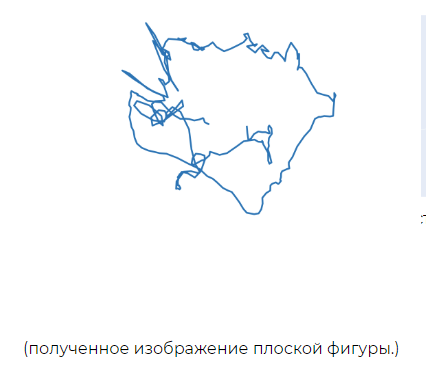
\includegraphics[scale = 1]{images_sav/2d_fig_img.png}}
\end{figure}
\subsection{Классификация данных (Савосин Артем, Макаров Максим)}

После проделанной выше работы - получение, фильтрация, выделение такта, нахождение среднего движения из нескольких тактов, перенос 3-х мерных данных в 2-х мерное изображение, остается только классифицировать полученный набор данных. 
\begin{figure}[H]
\center{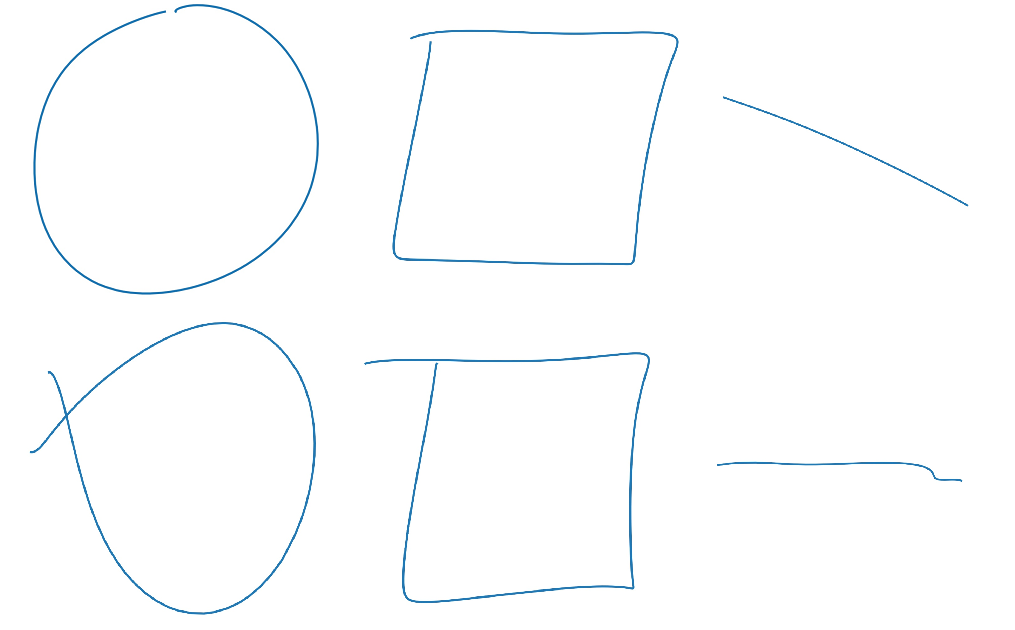
\includegraphics[scale = 1]{images_sav/data_examples.png}}
\end{figure}
Выше представлены примеры данных, полученных в ходе работы. Каждый ряд картинок отображает один из классов движений - круг, квадрат, встряска. Человеческий мозг легко бы справился с задачей распознать и классифицировать новое изображение, основываясь даже на таком небольшом количестве примеров. Легко можно заметить, что в классе кругов изображения будут примерно похожи на овалы, в классе квадратов можно наблюдать фигуру схожую с крестом, а изображения из класса встрясок похожи на линию. К сожалению, то, что понятно человеку, не так просто объяснить машине. Нашей команде понадобилось бы большое количество времени, чтобы описать все условия принадлежности той или иной фигуры к определенному классу, если бы нам вообще удалось это сделать. Решить задачу классификации мы сможем, применив сверточную нейронную сеть.
\subsubsection{Что такое нейронная сеть?}
Это математическая модель, изобретенная в ходе изучения работы мозга и попытке смоделировать его поведение. 
Мозг человека состоит из нейронов, соединенных между собой каналами, по которым передается электрический импульс. Нейроны получают сигналы от многих других нейронов, обрабатывают их, и посылают новый сигнал. 
Когда мы видим какое-то изображение, в зрительной коре головного мозга активируются строго определенные участки, которые передают сигнал далее, где он обрабатывается, и мы понимаем, что перед нами, скажем, круг, а не квадрат.
Компьютерная нейронная сеть - это попытка хотя бы частично воссоздать процесс, происходящий в голове в момент распознавания картинки.  Простая нейронная сеть состоит из нескольких слоёв. 
\begin{figure}[H]
\center{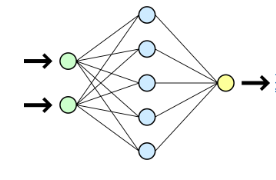
\includegraphics[scale = 1]{images_sav/neuro.png}}
\end{figure}

Входной слой (зеленый) - это “глаза” нашей сети.
 Скрытый слой (синий)
Выходной слой (желтый) - в этом слое ровно столько нейронов, сколько мы имеем классов изображений. А сила сигнала на том или ином нейроне говорит о том, насколько сильно входной объект похож на объект, за который отвечает этот нейрон.
\subsubsection{Что такое сверточная нейронная сеть?}
СНС состоит из разных видов слоев: сверточные (convolutional) слои, субдискретизирующие (subsampling, подвыборка) слои и слои «обычной» нейронной сети – персептрона.
Главное отличие такой сети - наличие сверточных слоев. Перед тем, как тренировать модель, изображение будет пропущено через ряд сверток - некоторое количество фильтров, позволяющих выделить характерные признаки изображения.
\subsubsection{Так как же сеть классифицирует изображения?}
Как я уже отмечал ранее, нейроны связаны между собой каналами. 
Входные нейроны связываются со скрытыми, скрытые с выходными. На каждой такой связи расставляются веса - насколько сильно важен для следующего нейрона входящий в него по этой связи нейрон. Далее каждый нейрон производит некоторые вычисления внутри себя, и передает сигнал далее.
Когда на вход подается изображение, входные нейроны задействуются, а сила сигнала, передаваемого ими, зависит от того, насколько яркая картинка в этом месте. Сигнал передается далее, происходят вычисления во внутренних слоях. После этого на каких-то выходных нейронах появится сигнал. Мы понимаем, какие выходные нейроны активны, и насколько они активны, и делаем вывод о принадлежности изображения к тому или иному классу.
\subsubsection{Тренировка нейронной сети.}
Нужно отметить, что при создании сети, веса между нейронами расставляются случайно - они никак не связаны с изображениями, которые мы хотим классифицировать. Далее мы прогоняем через такую сеть наши данные, и выявляем ошибки. На основе этих ошибок меняются веса связей, и мы снова прогоняем наши данные и смотрим, насколько хорошо классифицируется. Потом еще раз вносим коррективы в веса связей, и так далее. На каждом шаге обучения веса меняются с помощью функции оптимизации.



\subsection{Первый прототип классификатора (Максим Макаров)}
Также, несмотря на то что это не входило в список моих задач, я решил попробовать создать первый прототип классификатора обработанных данных.
% Моими основными задачами были доработка мобильного приложения и создание классификатора обработанных данных.
Так как обработанные данные есть ни что иное, как фигура на плоскости, было рассмотрено несколько вариантов классификации этих самых данных:
\begin{enumerate}
    \item Классифицировать фигуры без какой-либо дополнительной обработки
    \item Нормировать фигуры по максимальному отклонению от точки (0; 0)
    \item Построить графики с помощью программной библиотеки mathplotlib, после чего классифицировать полученные изображения
\end{enumerate}
В связи с тем, что классификация изображений является весьма распространенной задачей, то было решено выбрать следующую стратегию: строить графики показаний акселерометра с помощью программной библиотеки mathplotlib и классифицировать полученные изображения.

Таким образом, возникли следующие подзадачи:
\begin{enumerate}
    \item Построить графики с помощью программной библиотеки mathplotlib
    \item Классифицировать полученные изображения, используя методы машинного обучения
    \item Добавить вывод предсказаний в мобильное приложение
\end{enumerate}
Благодаря лабораторным работам по линейной алгебре имелся достаточно богатый опыт использования программной библиотеки mathplotlib, поэтому построение графиков не составило труда. Однако, необходимо было избавиться от посторонних данных на графиках, таких как шкалы и вспомогательные сетки, а также привести все данные к единому формату: квадратные изображения строго определенного размера, одинаковый масштаб по оси абсцисс и по оси ординат.

\begin{figure}[H]
    \begin{center}
        \begin{tabular}{cc}
            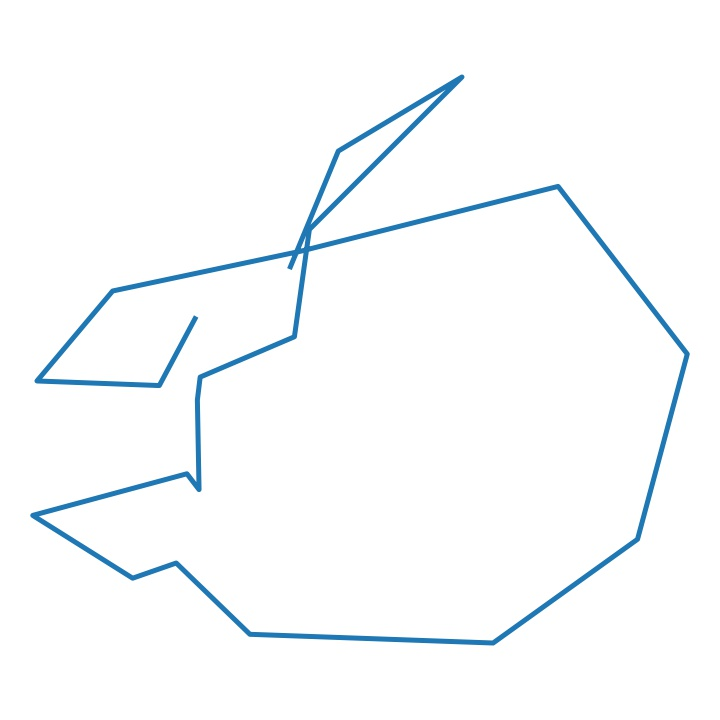
\includegraphics[width=0.4\textwidth]{max_kt2_images/image4.jpg} & 
            \includegraphics[width=0.4\textwidth]{max_kt2_images/image2.jpg} \\
        \end{tabular}
    \end{center}
    \caption{Примеры полученных изображений различных жестов: круг (слева), встряхивание (справа).}
\end{figure}

% Дополнительно, бонусом такого решения является то, что изображения нормируются по размеру автоматически.

Далее, я приступил к поиску подходящей программной библиотеки машинного обучения. Были рассмотрены следующие варианты:
\begin{enumerate}
    \item Theano -- библиотека численного вычисления в Python. Вычисления в Theano выражаются NumPy-подобным синтаксисом и компилируются для эффективных параллельных вычислений как на обычных CPU, так и на GPU.
    \item TensorFlow — открытая программная библиотека для машинного обучения, разработанная компанией Google для решения задач построения и тренировки нейронной сети с целью автоматического нахождения и классификации образов, достигая качества человеческого восприятия.
    \item Apache MXNet —  это программная платформа глубокого обучения с открытым исходным кодом, используемая для обучения и развертывания глубоких нейронных сетей.
\end{enumerate}

В связи с популярностью программной библиотеки TensorFlow и, как следствие, обилием готовых решений, основанных на ней, выбор был очевиден. Также данная библиотека является достаточно производительной, так как вся работа ведется с графами вычислений, операции с которыми, можно эффективно исполнять на некоторых типах процессоров.  Так как опыта работы с TensorFlow у меня не было совсем, первым делом было решено искать примеры проектов, сделанных на основе этой программной библиотеки. В процессе поиска я наткнулся на очень интересное решение от Google – Teachable Machine. Это инструмент, основанный на веб-технологиях, который делает обучение моделей быстрым, легким и доступным каждому, а также позволяет экспортировать полученные модели для интеграции в собственные решения.

\begin{figure}[H]
    \begin{center}
        \includegraphics[width=0.8\textwidth]{max_kt2_images/image10.png}
    \end{center}
    \caption{Интерфейс программы “Teachable Machine”.}
\end{figure}

В программе предустановлены 3 модели: для распознавания изображений, аудиозаписей и поз. Нас интересует первая модель – это сверточная нейронная сеть. Данный тип искусственных нейронных нейронных сетей хорошо зарекомендовал себя в задачах распознавания образов. Главное отличие сверточных нейронных сетей от обыкноневенного перцептрона, то есть полносвязной нейронной сети, в том, что она обучается на основе карт признаков, которые формируются в результате операций свертки матрицами весов различных фильтров. Сами же матрицы весов корректируются в процессе обучения методом обратного распространения ошибки.

\begin{figure}[H]
    \begin{center}
        \includegraphics[width=0.8\textwidth]{max_kt2_images/image7.png}
    \end{center}
    \caption{Типовая архитектура сверточной нейронной сети.}
\end{figure}

% Принцип работы Teachable Machine прост: в левом меню создаются классы и для каждого загружается набор тренировочных изображений или аудиозаписей в зависимости от выбранного ранее типа модели. При необходимости можно указать дополнительные параметры обучения (скорость обучения, количество эпох и т.д.), однако, как выяснилось позже, стандартные параметры обучения позволяют добиться достаточно неплохих результатов. Затем, полученную модель можно экспортировать в формате “.h5”.

Далее, нужно было определиться с классами движений. После совещания с другими участниками команды, мы остановились на том, что система будет уметь распознавать три типа жестов: круг, квадрат и встряхивание. Недолго думая, один из участников команды приступил к сбору датасета и уже через пару часов, в моих руках было 15 экземпляров “кругов”, 14 “квадратов” и столько же “встряхиваний”. Далее, данный набор данных был загружен в Teachable Machine, а также была запущена тренировка со стандартными настройками (50 эпох, batch size = 16, скорость обучения = 0,001).  После чего, модель была экспортирована для использования вместе с интерпретируемым языком программирования Python 3. Сразу же захотелось протестировать данную модель: из другого набора данных были выбраны несколько записанных ранее жестов в виде графиков, которые после стали входными данными для алгоритма распознавания. Были получены следующие результаты:

\begin{figure}[H]
    \begin{center}
        \begin{tabular}{cc}
            \includegraphics[width=0.35\textwidth]{max_kt2_images/image4.jpg} & 
            \includegraphics[width=0.35\textwidth]{max_kt2_images/image11.png} \\
        \end{tabular}
    \end{center}
    \caption{Исходное изображение круга (слева) и результат работы алгоритма (справа).}
\end{figure}

\begin{figure}[H]
    \begin{center}
        \begin{tabular}{cc}
            \includegraphics[width=0.35\textwidth]{max_kt2_images/image9.jpg} & 
            \includegraphics[width=0.35\textwidth]{max_kt2_images/image8.png} \\
        \end{tabular}
    \end{center}
    \caption{Исходное изображение встряхивания (слева) и результат работы алгоритма (справа).}
\end{figure}

\begin{figure}[H]
    \begin{center}
        \begin{tabular}{cc}
            \includegraphics[width=0.35\textwidth]{max_kt2_images/image3.jpg} & 
            \includegraphics[width=0.35\textwidth]{max_kt2_images/image1.png} \\
        \end{tabular}
    \end{center}
    \caption{Исходное изображение квадрата (слева) и результат работы алгоритма (справа).}
\end{figure}


\subsubsection{Модель}

В силу того, что описаная выше модель работает через web - интерфейс, а в нашем проекте требуется реализовать бибилотеку, которую можно развернуть у себя на устройстве, нам пришлось находить новое решение для классификации данных.
Как уже было описано ранее, в нашем проекте решено было использовать библиотеку tensorflow, имеющую обширное количество готовых решений, в том числе и для нейронной сети, которую можно запустить у себя на устройстве.

Для начала про данные - входные изображения разделены в пропорции 2 к 1 на тренировочные и валидационные. На первых модель обучается, вторые нужны для проверки на переобученность модели. 
Используя библиотеку keras preprocessing, мы нормируем все изображения так, чтобы входная матрица принимала цветовые значения не от 0 до 255, а от 0 до 1. Это требуется по причине того, что сети удобнее работать со значениями от 0 до 1. Далее в тренировочные данные добавляются измененные версии тренировочных файлов - изображения, повернутые на 45 градусов, Этот шаг нужен для того, чтобы избежать переобучения модели - ведь движения, записанные новым пользователем могут отличаться от собранных. 
Далее поговорим о самой модели и слоях, из которых она состоит
\begin{figure}[H]
\center{\includegraphics[scale = 1]{images_sav/model.png}}
\end{figure}
Входной слой состоит сверточного слоя ,который будет генерировать 32 фильтра для выделения параметров, за которым следует слой MaxPooling, который выделяет один, самый сильный сигнал из группы 3 на 3 и оставляет его, что позволяет значительно уменьшить изображение, сохранив его главные детали.  Далее повторим процесс, добавив новый сверточный слоев с большим количеством фильтров, таким образом, разбирая наше изображение на большое количество маленьких параметров, из которых складывается представление о фигуре.
Далее следуют слои обычной нейронной сети, с еще 516 фильтрами.
Последний слой состоит из 3 нейронов (по количеству классов) и активатора softmax. Активатор выбирает максимальное значение из трех нейронов, и присваивает ему весь сигнал, остальные нейроны будут пустыми. 

Про точность модели 
на финальном шаге обучения точность модели на обучаемых данных составила 97,92 процентов , а на независимых данных модель смогла угадать все 100 процентов представленных изображений. 
За два шага до этого модель укладывала 100 процентов всех тренировочных данных. \newline
Epoch 18/20 \newline
accuracy: 1.0000 - val-accuracy: 1.0000 \newline
Epoch 19/20\newline
accuracy: 1.0000 - val-accuracy: 0.9792\newline
Epoch 20/20\newline
accuracy: 1.0000 - val-accuracy: 0.9792\newline
\begin{figure}[H]
\center{\includegraphics[scale = 1]{images_sav/accuracy.png}}
\end{figure}
\subsubsection{Описание вычислительного эксперимента.}

Для определения наиболее подходящей классифицирующей модели для наших данных, было решено провести ряд экспериментов.

Первым экспериментом был замер точности простой модели, состоящей из 2 сверточных слоев, без каких бы то ни было поправок на переобучение.

\begin{figure}[H]
\center{\includegraphics[scale = 1]{images_sav/model1.png}}
\end{figure}

Для данной модели были выбраны 4 функции оптимизации:

\begin{itemize}
	\item Оптимизация Адама - это метод стохастического градиентного спуска, основанный на адаптивной оценке моментов первого и второго порядка.
	\item Adagrad - это оптимизатор с частотой обучения, зависящей от параметров, которая адаптируется в зависимости от того, как часто параметр обновляется во время обучения. Чем больше обновлений получает параметр, тем меньше обновлений.
	\item SGD - Стохастический градиентный спуск и оптимизатор импульса.
	\item Rmsprop
\end{itemize}

Данные генерировались с помощью простой функции, которая переводила матрицу со значениями от 0 до 255 в значения от 0 до 1.

Результаты работы предоставлены на графиках ниже.

\begin{figure}[H]
\center{\includegraphics[scale = 0.8]{images_sav/exp1.png}}
\end{figure}

Заметим, что все модели показывают довольно неплохую точность - распознавание тренировочных данных не ниже 99 процентов, валидационных - 95. Главное отличие в скорости достижения высокой точности и потерях нейронов в ходе обучения. Лучше всего себя показала модель с функцией оптимизации adam.

Обычно, при обучении нейронной сети главной проблемой является переобучение, в результате которого модель начинает очень хорошо распознавать изображения, на которых она обучалась, и гораздо хуже распознает новые изображения. Проверим, что будет с нашими моделями, если мы добавим в них методы, противодействующие переобучению. 

Добавим еще один сверточный слой и введем новые слои Dropout, которые выкидывают 20 процентов обученных нейронов на каждом шаге, что уменьшает риск переобучения.  
\begin{figure}[H]
\center{\includegraphics[scale = 1]{images_sav/model2.png}}
\end{figure}
Далее проверяем точность этих моделей на тех же 4 функциях.

\begin{figure}[H]
\center{\includegraphics[scale = 0.8]{images_sav/exp2.png}}
\end{figure}

Заметим, что графики стали более волатильными - возросло количество потерь, упала точность, теперь тренировочная точность лежит в пределах от 93 до 100, а валидационная - от 87 до 100. Лучше всех себя опять показала модель с оптимизатором adam. 

Добавим к данной модели еще несколько . Теперь тренировочные данные будут разбавляться набор из видоизмененных жестов - растянутых, повернутых на 45 градусов, смещенных относительно центра.
В силу того, что данных получится несколько больше, увеличим количество тренировочных шагов.
Прроверим эти нововведения на двух оптимизаторах - самом точном и стабильном на данный момент (adam) и самый волатильный (rmsprop)

\begin{figure}[H]
\center{\includegraphics[scale = 0.5]{images_sav/exp3.png}}
\end{figure}

На первых двух графиках показана точность работы модели с оптимизатором adam, а на вторых - c rmsprop. Заметим, что точность моделей очень сильно упала, особенно у второго классификатора. 

Исходя из проделанных экспериментов можно сделать следующий вывод - наши данные имеют очень своеборазную форму, которая довольно слабо отличается внутри класса, и ввод функций, изменяющих исходные данные, сильно искажает общие черты для класса, настолько, что становится гораздо сложнее их выделять.
Исходя из результатов экспериментов было решено ввести самый первый вариант модели с самой точной функцией оптимизатором.
\section{Часть Глеба}

Основной задачей являлось создание библиотеки для обработки жестов, с помощью которой можно обучать модель и распознавать движения. Все наработки находились в Jupyter файлах, поэтому было необходимо все перенести все в Python файлы, объединить и "причесать" код. \newline

Так как наше мобильное приложение сделано с помощью JavaScript, а все основные алгоритмы – с помощью Python, то было принято решение сделать следующее: разработать библиотеку с помощью JavaScript, которая предоставляет интерфейс для обучения и предсказания движения, а внутри эта библиотека общается с Python сервером с помощью протокола http, на котором уже происходят все вычисления.

\subsection{JavaScript Library}
У JavaScript библиотеки определены следующие классы:
\begin{itemize}
  \item GestureData. Данный класс характеризует данные, полученные с устройства.
  \item Gesture. Данный класс характеризует распознанный жест.
\end{itemize}
В класссе Gesture содержится информация о жесте:
\begin{itemize}
  \item name -- класс, к которому он принадлежит (круг, квадрат, встряска и т.д.)
  \item 2dProjection -- 2-мерная проекция движения в плоскости
  \item 3dProjection -- 3-мерное движение в пространстве
  \item gestureData -- данные с акселерометра и гироскопа
\end{itemize}

У JavaScript библиотеки определены следующие методы:
\begin{itemize}
  \item train(name: String, gesture: GestureData): Promise<null> {} 
  \item predict(gesture: GestureData): Promise<Gesture> {}
\end{itemize}
Эти методы сериализуют переданные аргументы в JSON формат и отправляют их на Python сервер.


\subsection{Python Server}
Основная обработка данных происходит на серверной части.

Вне зависимости от того, на какой эндпоинт пришел запрос, сервер всегда обрабатывает GestureData:
\begin{itemize}
  \item в первую очередь данные акселерометра фильтруются и сглаживаются (см. часть Фархата),
  \item после этого, показания акселерометра компенсируются, основываясь на данных гироскопа (см. часть Артема Самарина),
  \item затем, выделяются такты и ищется усредненное движение (см. часть Влада),
  \item далее, полагая, что движение совершается в какой-то двумерной плоскости, находится наилучшая плоскость, внутри которой которой уже происходит поиск и классификация движения.
\end{itemize}

На сервере предусмотрены следующее эндпоинты:
\begin{itemize}
  \item (POST) /train (name: String, gesture: GestrureData). При получении этого запроса, происходит обучение модели на основе полученного усредненного движения в плоскости, полагая, что данное движение соответсвует классу name (см. часть Артем Савосина) и при успешном обучении возвращается сообщение о успехе.

  \item (POST) /predict (gesture: GestureData). При получении этого запроса происходит классификация движения на основе существующей модели (см. часть Арема Савосина) и возвращается Gesture, в котором содержится класс и движение в плоскости и пространстве.
\end{itemize}

\subsection{Ссылка на библиотеку}
https://github.com/kaikash/hse-study-project
\newpage
\subsection{Мобильное приложение для сбора данных и тестирования, распознающее движения и восстанавливающее движение (Макаров Максим)}

\subsubsection{Первый прототип приложения}
% Моей основной задачей была разработка мобильного приложения для сбора данных и тестирования, которое также способно распознавать движения и восстанавливать их (строить изображения записанных движений).


% \subsection{КТ 1}
Изначально было решено реализовать функцию сбора данных. 
% Основной моей задачей была разработка приложения для сбора показаний акселерометра и гироскопа.
Нужно было определиться с платформой, на которой будет работать приложение. Так как одним из требований является кроссплатформенность, то есть приложение должно работать на разных операционных системах, было принято решение использовать один из фреймворков для разработки таких приложений.
% Я рассматривал следующие варианты:
% \begin{itemize}
%     \item Flutter -- SDK с открытым исходным кодом для создания мобильных приложений от компании Google. Он используется для разработки приложений под Android и iOS, а также это пока единственный способ разработки приложений под Google Fuchsia.
%     \item Xamarin -- платформа для разработки приложений для IOS и Android с помощью фреймворка .NET и языка программирования C\#.
%     \item React Native -- фреймворк от Facebook для разработки мобильных приложений с помощью языка программирования Javascript. 
%     \item Expo -- основанный на React Native фреймворк для разработки мобильных приложений с помощью языка программирования Javascript. Главное его отличие от React Native в том, что он содержит в себе практически все необходимые компоненты, которые обычно требуют дополнительной установки, а также удобную среду для разработки.
% \end{itemize}
% В связи с тем, что я имел достаточно большой работы с языком программирования Javascript, мною был выбран последний -- Expo.
Мною был выбран фреймворк Expo.
После прочтения документации к фреймворку, было несложно запустить среду для разработки, а автоматическое обновление приложения значительно ускорило процесс разработки.

Предполагался следующий способ взаимодействия с приложением: пользователь нажимает на кнопку и делает некоторый жест с телефоном в руке, после чего отпускает кнопку. Далее, записанные показания в виде JSON-файла можно отправить с помощью AirDrop, Telegram, электронной почты и т.д.
\begin{figure}[H]
    \begin{center}
        \begin{tabular}{ccc}
            \includegraphics[width=0.25\textwidth]{max_kt1_images/image2.png} & 
            \includegraphics[width=0.25\textwidth]{max_kt1_images/image3.png} & 
            \includegraphics[width=0.25\textwidth]{max_kt1_images/image1.png} \\
        \end{tabular}
    \end{center}
    \caption{Интерфейс первой версии приложения.}
\end{figure}

% \subsection{КТ 2}

\subsubsection{Доработка приложения }
Далее, было необходимо доработать мобильное приложение. Хотелось бы видеть результат распознавания сразу после записи какого-либо жеста, для чего было решено сделать http сервер на node.js и доработать мобильное приложение так, чтобы оно отправляло записанное движение на данный сервер, а сервер в свою очередь запускал алгоритм распознавания и возвращал результат его работы обратно в приложение.
\begin{figure}[H]
    \begin{center}
        \includegraphics[width=0.2\textwidth]{max_kt2_images/image5.jpg}
    \end{center}
    \caption{Интерфейс усовершенствованного мобильного приложения. Снимок экрана был сделан сразу после записи движения.}
\end{figure}

\subsubsection{Последняя версия}
Затем, в связи с наличием готовой библиотеки для обучения и распознавания жестов, разработанной одним из участников нашей команды, было решено все-таки переделать приложение, чтобы повысить удобство его использования. Пришлось практически полностью переработать интерфейс. Теперь приложение имеет две вкладки: тренировка и распознавание. Они отвечают, как следует из названия, за тренировку и распознавание соответственно.

Тестирование происходит следующим образом: зажимается кнопка \textit{Record} и выполняется движение. Далее приложение, используя программную библиотеку, получает результат распознавания. В результате чего на экране появляется изображение восстановленного жеста и предсказание алгоритма в виде надписи вида \textit{"I guess it's a <название жеста>"}. Далее, при желании можно нажать на кнопку \textit{Reset}, чтобы записать новый жест.
\begin{figure}[H]
    \begin{center}
        \begin{tabular}{ccc}
            \includegraphics[width=0.15\textwidth]{testingapp_screenshots/IMG_2011.PNG} & 
            \includegraphics[width=0.15\textwidth]{testingapp_screenshots/IMG_2016.PNG} & 
            \includegraphics[width=0.15\textwidth]{testingapp_screenshots/IMG_2017.PNG} \\
        \end{tabular}
    \end{center}
    \caption{Интерфейс тестирования в различных состояниях.}
\end{figure}

Процесс обучения немного отличается: жест записывается аналогичным образом, но после записи жеста появляются 3 кнопки: \textit{Reset, Submit} и \textit{Share}. Первая кнопка работает тем же образом, что и при тестировании, третья отвечает за отправку записанного жеста с помощью AirDrop, Telegram, электронной почты и т.д. При нажатии на кнопку \textit{Submit} записанные данные с помощью программной библиотеки отправляются на сервер, а он в свою очередь возвращает изображение жеста восстановленное из этих данных. Затем, оно появляется на месте кнопки записи жеста.
\begin{figure}[H]
    \begin{center}
        \begin{tabular}{cccc}
            \includegraphics[width=0.15\textwidth]{testingapp_screenshots/IMG_2012.PNG} & 
            \includegraphics[width=0.15\textwidth]{testingapp_screenshots/IMG_2013.PNG} & 
            \includegraphics[width=0.15\textwidth]{testingapp_screenshots/IMG_2014.PNG} & 
            \includegraphics[width=0.15\textwidth]{testingapp_screenshots/IMG_2015.PNG} \\
        \end{tabular}
    \end{center}
    \caption{Интерфейс обучения в различных состояниях.}
\end{figure}
\section{Заключение}
\subsubsection{Основные результаты:}
\begin{itemize}
    \item Разработано приложение по сбору и классификации данных гироскопа и акселерометра.
    \item Разработаны библиотека, состоящая из клиентской части, написанной на языке JavaScript и серверной, написанной на языке Python
    \item Разработан метод отображения движения телефона в 3D и последующей проекции в 2D для классификации.
    \item Разработан механизм выделения и усреднения тактов движений.
    \item Разработан механизм фильтрации данных.
    \item Разработан механизм распознавания движений.
\end{itemize}

\subsubsection{Перспективы дальнейшей работы:}
\begin{itemize}
    \item Перенос вычислений с сервера на телефон.
    \item Создание возможности добавления новых жестов.
    \item Увеличения производительности.
\end{itemize}
% \begin{thebibliography}{3}
%     \bibitem{ya.ru}
%     ya.ru
%     \bibitem{Vshivkov}
%     Григорьев Ю. В., Вшивков В. А., Федорук, М. П. Численное моделирование методами частиц в ячейках. --- Новосибирск : Издательство СО РАН. --- 2004. --- 360 c.
%     \bibitem{LiuLiu}
%     Liu G. R., Liu M. B. Smoothed particle hydrodynamics: a meshfree particle method. --- Singapore : World Scientific Publishing. --- 2003. --- 449 p.
% \end{thebibliography}

% даём указание на включение данного место в оглавление как секции (\section)
\addcontentsline{toc}{section}{Список используемой литературы}
 
%далее сам список используевой литературы
\begin{thebibliography}{}
    \bibitem{1} \href{http://www.cs.cornell.edu/courses/cs4758/2012sp/materials/hmm_paper_rabiner.pdf}{www.cs.cornell.edu}
    \bibitem{2} В. И. Левенштейн. Двоичные коды с исправлением выпадений, вставок и
    замещений символов. Доклады Академий Наук СССР, 1965. 163.4:845-848.
    \bibitem{2} Гасфилд. Строки, деревья и последовательности в алгоритмах. Информатика и
    вычислительная биология. Невский Диалект БВХ-Петербург, 2003.
    \bibitem{3} 4.	R. A. Wagner, M. J. Fischer. The string-to-string correction problem. J. ACM 21 1 (1974)
    \bibitem{4} \href{https://books.google.ru/books?id=iEO6AgAAQBAJ&pg=PA8&#v=onepage&q&f=false}{Алгоритмы и процессоры цифровой обработки сигналов.}
    \bibitem{5} \href{https://books.google.ru/books?id=s3H8s8rdsHkC&pg=PA83#v=onepage&q&f=false}{Digital Signal Compression: Principles and Practice.}
    \bibitem{6} \href{https://web.archive.org/web/20090708124031/http://mexman.ru/?p=6}{Теоретическая механика.}
    \bibitem{7} \href{http://journals.ioffe.ru/articles/viewPDF/8381}{Интепритиация измерений оптического гироскопа.}
    \bibitem{8} \href{https://habr.com/ru/post/105220/}{Хабр: Классификация данных методом опорных векторов.}
    \bibitem{9} \href{http://www.cs.cornell.edu/courses/cs4758/2012sp/materials/hmm_paper_rabiner.pdf}{A Tutorial in Hidden Markov Models and Selected Applications in Speech Recognition, LAWRENCE R. REBINER, FELLOW.}
    \bibitem{} \href{https://plotly.com/python-api-reference/generated/plotly.graph_objects.Figure.html}{plotly graph objects Figure}
    \bibitem{} \href{http://www.l3s.de/~anand/tir14/lectures/ws14-tir-foundations-2.pdf}{Periodicity Detection, Time-series Correlation, Burst Detection}
    \bibitem{} \href{https://www.dataq.com/data-acquisition/general-education-tutorials/fft-fast-fourier-transform-waveform-analysis.html}{FFT (Fast Fourier Transform) Waveform Analysis}
    \bibitem{} \href{https://statanaliz.info/statistica/korrelyaciya-i-regressiya/linejnyj-koefficient-korrelyacii-pirsona/}{Линейный коэффициент корреляции Пирсона}
    \bibitem{} \href{http://risktheory.novosyolov.com/topic_correl.htm}{Границы коэффициента корреляци}
    \bibitem{} \href{http://risktheory.novosyolov.com/ill_zerocorr.htm}{Зависимое распределение с нулевой корреляцией}
    \bibitem{} \href{https://s3.amazonaws.com/assets.datacamp.com/production/course_4267/slides/chapter2.pdf}{Autocorrelation Function}






\end{thebibliography}
\section{Приложения}

\begin{itemize}
    \item \href{https://github.com/kaikash/hse-study-project/new\_lib}{Библиотека для мобильных устройств}
    \item \href{https://github.com/kaikash/hse-study-project}{Драфт проекта}
\end{itemize}


\end{document}

